%!TEX program = lualatex
%% -*- fill-column: 120; indent-tabs-mode: nil; tab-width: 2; -*-
\documentclass[
  twoside,
  parskip=half-,
  %BCOR=0pt,
  %DIV=50,
  %14pt,
]{scrreprt}

\usepackage[ngerman]{babel}
\usepackage[utf8]{inputenc}
\usepackage[german=guillemets]{csquotes}
\usepackage{luacode}
\usepackage[dvipsnames, cmyk]{xcolor}
\usepackage{graphicx}
\usepackage{multicol}
\usepackage{tikz}
\usetikzlibrary{positioning, calc}
\usepackage{tikzpagenodes}
\usepackage{fancyvrb}
\usepackage{multicol}
\usepackage{enumitem}
\usepackage{longtable}
\usepackage{pdfpages}
\usepackage{tocloft}
\usepackage{array}
\usepackage{rotating}

\newcolumntype{L}[1]{>{\raggedright\let\newline\\\arraybackslash\hspace{0pt}}p{#1}}
\newcolumntype{C}[1]{>{\centering\let\newline\\\arraybackslash\hspace{0pt}}p{#1}}
\newcolumntype{R}[1]{>{\raggedleft\let\newline\\\arraybackslash\hspace{0pt}}p{#1}}


\newenvironment{linedbox}[2]{
  \par
  \def\linedboxtitle{#1}
  \def\linedboxcolor{#2}
  \color{#2!50!black}
  \begin{tikzpicture}[color=\linedboxcolor]
    \node[
      inner sep=0pt, 
      outer xsep=0pt,
      anchor=west,
      font=\bfseries\large,
    ] (A) {\linedboxtitle};
    \draw[
      line width=3pt,
      %line cap=round,
    ] ($(A.east) + (10pt, 0)$) -- (\textwidth - 5pt, 0);
  \end{tikzpicture}
 }{%
  \setlength{\parskip}{0pt}%
  \par%
  \begin{tikzpicture}[color=\linedboxcolor]
    \draw[
      line width=3pt,
      %line cap=round,
    ] (0, 0) -- (\textwidth - 5pt, 0);
  \end{tikzpicture}
}

%\newenvironment{praxis}{\begin{linedbox}{Bezug zum geplanten Angebot}{MidnightBlue}}{\end{linedbox}}
%\newenvironment{beispiel}{\begin{linedbox}{Fallbeispiel}{green}}{\end{linedbox}}

\usepackage[framemethod=tikz]{mdframed}
\newmdenv[
  linewidth=3pt,
  topline=false,
  bottomline=false,
  rightline=false,
  frametitlefont={\Large\bfseries},
  % frametitlebackgroundcolor=SeaGreen!20!white,
  linecolor=ForestGreen!50!white,
  innertopmargin=10pt,
  frametitleaboveskip=7pt,
  frametitlebelowskip=7pt,
  skipabove=10pt,
  apptotikzsetting={\tikzset{mdfframetitlebackground/.append style={
    left color=ForestGreen!50!white,
    right color=white,
  }}},
  frametitle={Fallbeispiel},
]{beispiel}

\newmdenv[
  linewidth=3pt,
  topline=false,
  bottomline=false,
  rightline=false,
  frametitlefont={\Large\bfseries},
  % frametitlebackgroundcolor=SeaGreen!20!white,
  linecolor=NavyBlue!50!white,
  innertopmargin=10pt,
  frametitleaboveskip=7pt,
  frametitlebelowskip=7pt,
  skipabove=10pt,
  apptotikzsetting={\tikzset{mdfframetitlebackground/.append style={
    left color=NavyBlue!50!white,
    right color=white,
  }}},
  frametitle={Bezug zum geplanten Angebot},
]{praxis}

\usepackage{fontspec}
\defaultfontfeatures{Ligatures=TeX}
\setsansfont{SourceSansPro-Light}[
  BoldFont = SourceSansPro,
  ItalicFont = SourceSansPro-Light-it,
]
\renewcommand{\familydefault}{\sfdefault}

\usepackage{relsize}

\usepackage[
  hidelinks,
  breaklinks=true,
]{hyperref}
\def\UrlFont{\sffamily\smaller}

\usepackage[german=guillemets]{csquotes}
\renewcommand{\mkccitation}[1]{\normalfont\newline\hbox{}\hfill #1}
\AtBeginEnvironment{displayquote}{\itshape}
\renewcommand{\mkenddispquote}[2]{\allowbreak\mbox{}\nobreak\hfill\hbox{\normalfont #2}}

\usepackage[
  style=authoryear-icomp,
  backend=biber,
  doi=false,
  isbn=false,
  ibidtracker=constrict,
  pagetracker=page,
  useprefix=true,
]{biblatex}

\DeclareNameAlias{sortname}{last-first}
\DefineBibliographyStrings{german}{
  urlseen = {abgerufen am},
}
\defbibheading{bibliography}[\bibname]{%
  \addchap{#1}% 
  \pagestyle{scrplain}%
}
\renewbibmacro*{date}{%
  \printdate
  \iffieldundef{origyear}{%
  }{%
    \setunit*{\addspace}%
    \printtext[parens]{orig. \printorigdate}%
  }%
}

\addbibresource{quellen.bib}
\setlength{\bibitemsep}{2ex}

\renewcommand*\dictumwidth{0.8\linewidth}
\setkomafont{dictumauthor}{\normalfont}
\renewcommand*{\dictumauthorformat}[1]{#1}

\sloppy

\title{Planung eines personzentrierten Psychoedukations- und Beratungsangebots für Menschen mit chronischen Schmerzerkrankungen}
\subject{Bachelorarbeit}
\author{Sandra Hackenberg}

\colorlet{mycol}{black}
\begin{document}
\begin{titlepage}
  \begin{tikzpicture}[remember picture, overlay]
    \node[
      inner sep=-2pt,
      xshift=3cm,
      yshift=8cm,
      anchor=north west,
      color=mycol,
      font=\fontsize{35pt}{35pt}\selectfont\bfseries,
      align=left,
    ] at (current page.west) (title) 
    {Planung eines \\
    personzentrierten \\
    Psychoedukations- und\\
    Beratungsangebots \\
    für Menschen mit \\
    chronischen\\
    Schmerzerkrankungen};

    \node[
      inner sep=0pt,
      above=20pt of title.north west,
      anchor=south west,
      color=mycol,
    ] (pretitle) {Bachelorarbeit};

    \node[
      inner sep=0pt,
      below=2cm of title.south west,
      anchor=north west,
      font=\large,
      color=mycol,
      align=left,
    ] (author) {
      Sandra Hackenberg, Matrikelnummer 1189082\\[10pt]
      \normalsize 
      Erstprüferin: Nicole Luthardt M.A.\\
      Zweitprüferin: Dr. Verena Schurt\\[10pt]
      Eingereicht am 5. Januar 2022
    };

    \node[
      inner sep=0pt,
      xshift=3cm,
      yshift=-1cm,
      anchor=north west,
    ] at (current page.north west) {
      
\includegraphics[height=1.5cm]{unia_logo.pdf}
    };
    
    \node[
      inner sep=0pt,
      xshift=-3cm,
      yshift=-2.5cm,
      anchor=south east,
    ] at (current page.north east) {
      Lehrstuhl für Erwachsenen- und Weiterbildung
    };

    \node[
      inner sep=0pt, 
      anchor=south,
      yshift=3cm,
      ] at (current page.south){
\includegraphics[height=5.5cm]{ExtendedCommunityCircle.pdf}};
  \end{tikzpicture}
\end{titlepage}

\addtocontents{lof}{\protect\contentsline {figure}{%
  \protect\numberline {Titel}{\ignorespaces \url{https://openclipart.org/download/170352/ExtendedCommunityCircle.svg}\newline%
  (Creative Commons Zero 1.0 Public Domain License)}}{0}{}%
}

\makebox{}
\vfill
\dictum[Carl Rogers, \textit{A way of being} (1980)]{\itshape\large
  Vielleicht der Hauptgrund, warum ich bereit bin, Wagnisse einzugehen, ist meine Erfahrung, dass ich dabei, ob ich nun Erfolg habe oder scheitere, etwas \emph{lerne}.
  Lernen, insbesondere Lernen aus Erfahrung, ist eines der Hauptelemente, die mein Leben lebenswert gemacht haben.
  Solches Lernen hilft mir, über mich hinaus zu wachsen.
  
  Deshalb fahre ich fort, Risiken einzugehen.}
\vspace*{20pt}

\clearpage
 
\tableofcontents

\addchap{Einleitung}

\begin{beispiel}
  Ein 70-jähriger Patient steht zum dritten Mal in diesem Monat vor dem Tresen einer Facharztpraxis, bei der er schon viele Jahre in Behandlung ist. Er hält einen gefüllten Aktenordner unter dem Arm. Auf die Frage, warum er denn wieder hier sei, sein nächster Termin sei doch erst in vier Wochen, erzählt er: \textquote{Ich war zwei Wochen in der Schmerzklinik, aber es geht mir genauso schlecht wie zuvor. Die Schmerzen sind unerträglich! In der Klinik bekam ich nach der Ankunft einen Stundenplan vorgesetzt, wie bei meiner Schmerz-Reha vor zehn Jahren. Während der zwei Wochen hört man den Ärzten zu, wie sie Vorträge halten und Ratschläge geben. Zur Psychologin bin ich nur einmal gegangen - als sie anfing, mir zu sagen, ich müsse mich nur anders verhalten und meine Gedanken ändern, dann würden die Schmerzen auch besser, hatte ich genug davon. Ich bin doch nicht krank im Kopf, sondern im Rücken. Überhaupt wussten alle immer, was angeblich gut für mich ist: Die Ärzte, die Physiotherapeutinnen, die Psychologin, die Pflegekräfte... ohne dass sie mich gefragt hätten. Nach zwei Wochen wird man dann entlassen und muss wieder alleine zurecht kommen. Das war nun schon meine dritte Klinik, und ihr seid die achte Praxis, bei der ich in Behandlung war. Trotzdem wird es immer schlimmer. Meine erwachsenen Söhne laden mich nicht mehr zu Familienfeiern ein, weil ihnen mein Gerede über die Krankheit auf die Nerven geht. Es versteht eben niemand, wie es mir geht! Nur zu euch kann ich immer wieder kommen; ihr hört mir wenigstens zu.}
  \end{beispiel}
  
  Schmerzen - und insbesondere chronische, also lang anhaltende Schmerzen - dürften eines der größten Themen in der Humanmedizin überhaupt sein, einerseits aufgrund der Häufigkeit ihres Vorkommens (Prävalenz), andererseits aufgrund der zum Teil massiven Einschränkung der Lebensqualität eines Menschen, der an Schmerzen leidet. 
  
  \begin{displayquote}[{\cite{Schmerzgesellschaft}}]
    In jedem dritten Haushalt in Europa lebt ein Mensch, der unter Schmerzen leidet. Etwa 17 \% aller Deutschen sind von lang anhaltenden, chronischen Schmerzen betroffen – also mehr als 12 Millionen Menschen. Durchschnittlich dauert ihre Leidensgeschichte sieben Jahre, bei mehr als 20\% über 20 Jahre.
  \end{displayquote}
  
  Diese Zahlen beziehen sich auf eine Studie von \textcite{HeftSchmerz28}.
    Andere Autor:innen sprechen von 23 Millionen chronisch Schmerzkranken \autocite[vgl.][4]{wachter}.\footnote{Es ist aufgrund der Alterung der Gesellschaft davon auszugehen, dass die Anzahl ständig zunimmt; 1999 sprach man noch von 7 - 8 Millionen Erkrankten \autocite[vgl.][17]{glier}.}
    Immer wieder wird auch auf die hohen Kosten hingewiesen, die dem solidargemeinschaftlich finanzierten Gesundheitssystem dadurch entstehen (ungefähr 38 Mrd. Euro jährlich \autocite[vgl.][]{Schmerzgesellschaft}).
    Gleichzeitig ist ein \textbf{Versorgungsdefizit} dieser Menschen allgemein bekannt \autocite[vgl.][]{Nachbessern}.
    Eine Schmerzerkrankung stellt für Betroffene eine enorme Herausforderung körperlicher, emotionaler und sozialer Art dar: \textquote[{\cite[336]{HeftSchmerz5}}]{Chronischer Schmerz vermag die Grundfeste der Existenz zu erschüttern}. Es erfordert ein hohes Maß an Wissen und Können, um sich im Gesundheitssektor insgesamt zurecht zu finden und sog. \textit{Copingstrategien} zu entwickeln, also Maßnahmen aller Art, um mit dem Schmerz (weiter) zu leben.
    Gleichzeitig zeigen Studien, \textquote[{\cite[Schaeffer, Berens und Vogt 2017, zit. n.][]{BZGABeratungEdukation}}]{dass die Gesundheitskompetenz in Deutschland nicht sehr gut ausgeprägt ist: mehr als die Hälfte der Bevölkerung weist hier eine geringe Gesundheitskompetenz auf.}.
    Obwohl es zahlreiche medizinische Angebote für Menschen mit chronischen Schmerzen in Deutschland gibt, ist die Zufriedenheit mit der Behandlung erschreckend schlecht:
    Rund ein Drittel zeigte sich in o.g. Studie in Bezug auf die aktuelle Schmerztherapie als \textquote{(sehr) unzufrieden} \autocite[vgl.][]{HeftSchmerz28}.

    Bei hoher Prävalenz einer stark beeinträchtigenden Erkrankung und einer gleichzeitig niedrigen Gesundheitskompetenz der Betroffenen sowie einer mangelhaften Zufriedenheit mit der Behandlung insgesamt erscheint es dringend notwendig, neue Ideen in das weite Feld der Schmerzpatient:innenversorgung einzubringen. Die sogenannte \textbf{Psychoedukation} (\autoref{psychoedukation}) hat sich als \textquote[{\cite[60]{glier}}]{hoch wirksame Intervention} erwiesen, sie \textquote[{\cite[289]{quovadis}}]{zählt zum allgemeinen Standard}. Im ambulanten Bereich der medizinischen Versorgung gerät die Psychoedukation jedoch häufig in den Hintergrund, denn  \textquote[{\cite[289]{quovadis}}]{[i]m Tagesgeschäft werden immer wieder aktuelle Krisen den Vorzug vor der systematischen psychoedukativen Erarbeitung des Krankheitsbilds erhalten müssen.} Dabei haben Metaanalysen für bestimmten Patient:innengruppen bestätigt, dass durch psychoedukative Gruppenprogramme  \textquote[{\cite[Lincoln et al. 2007; Xia et al. 2011 zit. n.][289]{quovadis}}]{signifikante Effekte auf Rezidivrate, [stationäre - SH] Wiederaufnahmen, psychopathologische Störungen und auch die Lebensqualität erzielt werden können.}

    Um die Versorgungslage von Menschen mit chronischen Schmerzen im ambulanten Bereich zu verbessern entstand die \textbf{Idee}, Schmerzpatient:innen mittels systematisch durchgeführter Psychoedukation zu schulen und ihnen Wissen und Fähigkeiten zu vermitteln, die ihnen helfen, ihre Lebensqualität trotz der Schmerzerkrankung zu steigern. Für dieses Vorhaben soll eine fundierte pädagogische und didaktische theoretische Konzeption erarbeitet werden.
    
    Die Patient:innen sollen aber nicht nur neues Wissen und Können erlernen, sondern auch mit Blick auf die psychischen Anteile der Erkrankung beratend in Einzelgesprächen begleitet werden. Dazu wurde nach einem theoretischen Konzept gesucht, welches sowohl für den medizinischen als auch für den psychologischen und den pädagogischen Bereich herangezogen werden kann. Ideal wäre ein Konzept, das sich ganz auf die Person mit all ihren Stärken und Schwächen, in ihrem Krank-sein und Gesund-sein, konzentriert. Denn Medizin, Psychologie und Pädagogik als gesellschaftliche Teilbereiche machen einen Wandel durch, der für die gesamte westliche Gesellschaft kennzeichnend ist, und das schon seit langer Zeit: \textquote[{\cite[13]{rogers1942}}]{Das ständig wachsende Interesse am Individuum und seiner Anpassung ist vielleicht eines der auffallendsten Phänomene unserer Zeit}. Dies schrieb der Psychologe Carl Rogers noch während der Zweite Weltkrieg tobte; seither hat sich diese Tendenz, den Blick auf den einzelnen Menschen, sein Wesen und seine Bedürfnisse zu richten, stetig weiter fortgesetzt. Sein Ansatz der \textbf{personzentrierten Gesprächspsychotherapie} findet sich bereits 1998 in der schmerzmedizinischen Fachliteratur als Grundlage der Kommunikation zwischen Therapeut:in und Patient:in \autocite[vgl.][62-65]{schmerztherapie} und wird auch in jüngerer Zeit von Schmerzmediziner:innen aufgegriffen \autocite[vgl.][]{fussnegger}.
    Der personzentrierte Ansatz rückt daher ins Blickfeld für das Angebotsvorhaben. Für Rogers basieren sowohl die therapeutische als auch die pädagogische Beziehung auf denselben wichtigen Grundbedingungen Kongruenz, Empathie und Wertschätzung und sind auf dasselbe Ziel ausgerichtet: die Entfaltung der Persönlichkeit. 

Die Herausforderung besteht nun also darin, ein kombiniertes Psychoedukations- und Beratungsangebot für (erwachsene) Menschen mit chronischen Schmerzerkrankungen zu entwickeln. Die vorliegende Arbeit beschäftigt sich daher mit der Aufgabe, ein solches Bildungsangebot zu planen. Dabei wird der \textbf{Schwerpunkt auf erwachsenenpädagogischen Fragen} liegen: Wie können mit pädagogisch-didaktischen Mitteln optimale Bedingungen geschaffen werden, damit die Lernenden frei gewählte, auf ihre individuellen Bedürfnisse zugeschnitte Lernziele erreichen können? Welche persönliche Haltung müssen Dozent:innen mitbringen, um zu Lernbegleiter:innen (\textit{facilitators} im Sinne Carl Rogers') zu werden? Und wie muss die Beziehung zwischen Pädagog:innen und Lernenden gestaltet werden, um den größtmöglichen Lernerfolg zu erzielen?

Doch bevor mit der aufwändigen Planung begonnen wird muss geklärt werden, ob nicht bereits bestehende Angebote den Bildungsbedarf der Schmerzpatient:innen ausreichend abdecken können. Zu diesem Zweck wird die Versorgungslage im Raum Augsburg an einigen Beispielen exemplarisch dargestellt. Einfache, ebenfalls beispielhafte Berechnungen werden zeigen, inwiefern ein neuartiges Angebot einen Beitrag zur Verbesserung der aktuellen Situation leisten kann und welche Vorteile es für Patient:innen haben kann.

Sobald festgestellt wurde, dass die Entwicklung eines neuen Bildungsangebots lohnend ist, kann mit der Planung begonnen werden. Hierfür werden zunächst die theoretischen Konzepte hinter den Begriffen \textit{Psychoedukation} und \textit{Beratung} untersucht. Diese und ihnen nahestehende, sich zum Teil überschneidende weitere Begriffe werden definiert, ihre wichtigsten Unterschiede und Gemeinsamkeiten dargestellt. Die Bedeutung und die Ziele von Psychoedukation und Beratung in der Medizin werden erläutert und es wird ein Bezug zur Erwachsenenpädagogik hergestellt. 

Das dritte Kapitel widmet sich dem personzentrierten Ansatz wie er von Carl Rogers und seinen Kollegen über viele Jahrzehnte praktischer psychologischer Forschung entwickelt und weiterentwickelt wurde. Der Entstehungszusammenhang gibt auch einen kurzen Überblick über Rogers' biografischen Hintergrund. Im Anschluss werden die wichtigsten Grundzüge und Begrifflichkeiten seiner sehr komplexen Theorie der menschlichen Persönlichkeitsentwicklung und der Wirksamkeit von Psychotherapie zusammengefasst dargestellt und herausgearbeitet, inwiefern die Beziehung einen zentralen Stellenwert in Rogers' Theorie sowohl in Bezug auf die Therapie als auch auf die Pädagogik hat.

Das nächste Kapitel möchte eine Synthese herstellen zwischen verschiedenen theoretischen Strömungen aus Medizin, Pädagogik und Psychologie. Es soll gezeigt werden, wie Aspekte der integrativen Medizin, der konstruktivistischen und subjektorientierten Pädagogik und des personzentrierten Ansatzes miteinander verbunden werden können.

Diese Synthese bildet dann die Basis für das didaktische Konzept des Angebots, welches im folgenden Kapitel entworfen wird. Dafür werden zunächst die Begriffe \textit{Programm} und \textit{Angebot} voneinander abgegrenzt und es werden Überlegungen angestellt, was es mit \textit{Bildungsbedürfnissen} und \textit{Bildungsbedarfen} auf sich hat und wie diese ermittelt werden können. Dann erfolgt eine Darstellung der drei Schritte der Angebotsplanung, wobei auf den ersten Schritt, die Planungsphase, das Hauptaugenmerk gelegt wird.

Anschließend wird ein detailliertes didaktisches Konzept des geplanten Angebots entworfen. Anhand von W-Fragen werden alle wichtigen Aspekte beleuchtet, die geklärt sein müssen ehe ein Angebot in die Umsetzungsphase übergeht. Am Ende dieses Kapitels stehen ein Strukturplan sowie ein Verlaufsplan des Angebots sowie ein Ausblick auf die Phasen der Angebotsumsetzung und -verbesserung, die auf die Planung folgen müssen. Zudem werden einige Ideen angeführt, wie das geplante Angebot weiterentwickelt oder wissenschaftlich untersucht werden könnte.

\paragraph{Anmerkung zu den Fallbeispielen}In dieser Arbeit werden immer wieder Fallbeispiele angeführt, um den Leser:innen einen Eindruck zu geben, wie Beratungsgespräche ablaufen können und wie sich die krankheits- und persönlichkeitsbezogene Entwicklung von Schmerzpatient:innen gestalten kann. Die Darstellung der Personen und ihrer Geschichten wurde allerdings so verfremdet, dass die Anonymität gewahrt bleibt. Zum Teil setzen sich die Fallbeispiele auch aus Erfahrungen zusammen, welche die Verfasserin in ihrer beruflichen Tätigkeit als Medizinische Fachangestellte mit mehreren verschiedenen Betroffenen gemacht hat. Insgesamt zeigen die Fallbeispiele also exemplarische Fälle, welche einerseits das \textquote{Typische}, das Verbindende, das die Geschichten vieler an chronischen Schmerzen erkrankten Menschen eint, zeigen. Gleichzeitig sollen sie sichtbar machen, dass unbedingte Wertschätzung und der Respekt vor der Individualität jeder Person Schlüssel sind, um signifikantes Lernen im Sinne Carl Rogers' zu ermöglichen \autocite[vgl.][153f.]{rogersLernenFreiheit}.

\begin{beispiel}
  Die Leser:innen erkennen die Fallbeispiele an dieser optischen Darstellung.
\end{beispiel}

\paragraph{Anmerkung zum inhaltlichen Aufbau dieser Arbeit} Ziel dieser Arbeit ist es, die Planung erwachsenenpädagogischer Bildungsangebote theoretisch zu reflektieren und diese Überlegungen in der Planung eines konkreten Angebots direkt anzuwenden. Daher bietet es sich an, Planungs-Theorie und Planungs-Praxis auch innerhalb des Textes dieser Arbeit eng miteinander zu verschränken. In Kapitel 3 sind diejenigen Textabschnitte, welche sich auf das geplante Beratungs- und Edukationsangebot für Menschen mit chronischen Schmerzerkrankungen beziehen, daher optisch (farblich und grafisch) abgesetzt. Auf diese Weise werden die einzelnen Bestandteile des Planungshandelns zunächst allgemein aus erwachsenenpädagogischer Sicht beleuchtet und im Anschluss auf eine bestimmte Angebotsidee bezogen dargestellt.
\begin{praxis}
  Die in diesem Format gesetzten Texte beziehen sich also auf das konkrete Angebot mit dem Arbeitstitel \textit{Beratungs- und Psychoedukationsangebot für Menschen mit chronischen Schmerzerkrankungen}.
\end{praxis}

\paragraph{Anmerkung zur Angebotsidee}

Damit sich Leser:innen dieser Arbeit im Text gut zurecht finden sei hier die Angebotsidee grob umrissen:
\begin{itemize}
  \item Zielgruppe: erwachsene Schmerzpatient:innen
  \item Bildungs- und Beratungsangebot: persönliche Beratung und Psychoedukation in Einzel- und Gruppensitzungen 
  \item Langfristige Begleitung, ca. 6 Monate
  \item Ambulantes Angebot, d.h. Durchführung in einer Haus- oder Facharztpraxis durch Medizinische Fachangestellte mit Zusatzqualifikation
  \item Personzentrierter Ansatz als Basis der theoretischen Konzeption
\end{itemize}

Diese Eckpunkte bilden den Ausgangspunkt für alle folgenden Überlegungen und das konkrete Planungshandeln.


\chapter{Wozu ein neues Angebot?}

Ganz am Anfang der Angebotsplanung steht die Idee für ein Bildungsangebot. Diese Idee besteht aus einer ungefähren Vorstellung darüber, an wen sich das Angebot richten kann, wie es ablaufen könnte und welche Inhalte thematisiert werden sollen. Diese Idee weiter auszuarbeiten - also Informationen über die Zielgruppe einzuholen, ein schriftliches didaktisches Konzept zu erarbeiten usw. - erfordert einen hohen Aufwand. Es ist daher der logische erste Schritt, sich zu fragen, ob nicht bereits ein vergleichbares Angebot existiert, wie sich das Angebot, das bisher nur als Idee existiert, von diesen bestehenden abheben könnte und welchen Mehrwert es für die Zielgruppe darstellen würde.

\section{Verortung im Umfeld bestehender Angebote im Raum Augsburg}

Patient:innen mit chronischen Schmerzerkrankungen können sich in der Stadt Augsburg und im Umland an verschiedene Praxen und Einrichtungen wenden.\footnote{Die Angaben in diesem Abschnitt beziehen sich auf Ergebnisse von Online-Recherche mit der Google-Suchmaschine sowie auf dem Online-Portal www.jameda.de (Stichworte \textquote{Schmerztherapie Augsburg}) vom Oktober 2021 sowie auf telefonische Anfragen an die sechs genannten Einrichtungen, welche die Verfasserin im Oktober 2021 an diese gerichtet hat. Schriftliche Notizen zu diesen Gesprächen s. Anhang.} Es gibt im Raum Augsburg nur drei Facharztpraxen, die auf Schmerzmedizin spezialisiert sind (Ärzt:innen mit dem Zusatz \textit{Spezielle Schmerztherapie}).\footnote{Einige Praxen und Kliniken mit orthopädischem Schwerpunkt bieten Schmerztherapie begleitend an, natürlich nur bei Vorliegen einer orthopädischen Ursache.} Von diesen speziell schmerztherapeutischen Praxen bietet eine ein ambulantes Programm zur multimodalen Schmerztherapie in den Praxisräumen an; dieses beschränkt sich auf eine Dauer von drei Wochen.

Ein \textbf{multimodaler Ansatz} bedeutet in der Schmerztherapie, dass Patient:innen je nach Art ihrer Erkrankung von einem Team aus Ärzt:innen, Physiotherapeut:innen und Psychotherapeut:innen behandelt werden. Bei einer multimodalen Schmerztherapie werden in der Regel die medizinische Therapie optimiert, z.B. Medikamente neu eingestellt, ein physiotherapeutisches Bewegungs- und Übungsprogramm durchgeführt sowie einige psychotherapeutische Gespräche geführt. Ergänzend erfolgen edukative Lerneinheiten, meist in Vortragsform, zu verschiedenen Themen \autocite[vgl.][99]{nobisHerausforderung}. Die Deutsche Schmerzgesellschaft definiert auf ihrer Website den Begriff \textit{Multimodale Schmerztherapie} folgendermaßen: 
\begin{displayquote}[{\cite[]{Schmerzgesellschaft}}]
  Ein eng unter den beteiligten Berufsgruppen abgestimmtes, individuelles Behandlungskonzept aus medikamentöser, psychologischer und Physiotherapie. Häufig werden Elemente des Entspannungs-/Bewegungstrainings und der Ergotherapie einbezogen. Die mehrwöchige Therapie beinhaltet die aktive Mitwirkung des Patienten.
\end{displayquote}

Die interdisziplinär ausgerichtete multimodale Schmerztherapie ist noch immer eher die Ausnahme als die Regel in der Gesundheitsversorgung \autocite[99]{nobisHerausforderung}. 
\begin{praxis}
  Das geplante Angebot wird \textbf{keine} multimodale Schmerztherapie sein. Dennoch gibt es Überschneidungspunkte, vor allem in dem Bestreben, einen ganzheitlichen Ansatz umzusetzen und medizinische, psychologische und edukative Elemente miteinander zu verbinden; sowohl der multimodale Ansatz als auch derjenige, der dem geplanten Angebot zu Grund liegen wird, sind dem bio-psycho-sozialen Modell verpflichtet. Die Verfasserin konnte im Raum Augsburg kein bestehendes Angebot ausfindig machen, welches dem geplanten gleicht oder ähnlich ist. Daher werden einzelne bestehende Angebote multimodaler Schmerztherapie herangezogen, um darzustellen, welche Vorteile das geplante Angebot für Betroffene haben könnte.
\end{praxis}

Als weitere wichtige Stellen, an denen Schmerzpatient:innen Hilfe finden können, werden in der Literatur \autocite[vgl.][Kap. 7]{nobisHerausforderung} u. a. Selbsthilfegruppen\footnote{In einer Selbsthilfegruppe findet ein Austausch unter Betroffenen und keine von medizinisch und/oder pädagogisch qualifiziertem Fachpersonal durchgeführte Psychoedukation oder Beratung statt. Daher fließen diese nicht in die Ausführungen in diesem Abschnitt mit ein.}, Schmerzambulanzen/Schmerz-Tageskliniken, Schmerz-Rehakliniken sowie Pain Nurses (vgl. \autoref{sec:wer}) genannt. Im Folgenden werden einige dieser Einrichtungen im Raum Augsburg beispielhaft dargestellt, damit Leser:innen sich einen Eindruck verschaffen können, welche Angebote bereits bestehen und wie es um den Zugang zu diesen Angeboten bestellt ist.

Da die \textbf{Schmerztagesklinik} in Augsburg Anlaufpunkt für viele Betroffene in Augsburg Land und Stadt ist, betragen die Wartezeiten auf ein Erstgespräch derzeit (10/2021) ca. zwei Monate, die Aufnahme in eine Therapiegruppe ist ab einer Wartezeit von fünf Monaten möglich. Das tagesklinische Programm läuft über 5 Wochen (5x wöchentlich, ca. 7 Stunden täglich), die Patient:innen verbringen den Tag in der Klinik und gehen über Nacht bzw. übers Wochenende nach Hause. Ein halbes Jahr nach Abschluss des Programms gibt es eine einwöchige \textquote{Refresher}-Gruppe. Danach endet die Betreuung.\footnote{\url{https://www.uk-augsburg.de/kliniken-und-institute/klinik-fuer-anaesthesiologie-und-operative-intensivmedizin/schmerztherapie/interdisziplinaere-schmerztagesklinik.html}, abger. am 07.12.21}

Als Beispiel für eine schmerztherapeutische \textbf{Rehabilitationseinrichtung} kann das Schmerztherapiezentrum Bad Mergentheim stehen (Fachklinik für Spezielle Schmerztherapie und Schmerzpsychotherapie). Sie ist von Augsburg in etwas über zwei Fahrtstunden mit dem Auto erreichbar. Ab Genehmigung des Reha-Antrags durch die Krankenkasse (welche in der Regel mehrere Wochen dauert) beträgt die Wartezeit auf einen Platz drei bis vier Monate, der Aufenthalt dauert durchschnittlich vier bis sechs Wochen. Ein ambulantes Nachbetreuungsangebot besteht dort nicht.\footnote{\url{https://www.schmerzklinik.com/}, abger. am 07.12.21}

Im \textbf{Schmerzzentrum} Starnberger See in Feldafing können Patient:innen nach einer Wartezeit von ca. vier bis fünf Wochen einen ungefähr zweiwöchigen stationären Aufenthalt antreten und ein multimodales Schmerztherapieprogramm durchlaufen. Im Anschluss ist eine tagesklinische oder alltagsbegleitende Fortführung möglich für maximal fünf Wochen (1-2x wöchentliche Treffen in der Tagesklinik).\footnote{\url{https://www.klinik-feldafing.de/behandlung/schmerzmedizin}, abger. am 07.12.21}

\begin{praxis}
  \paragraph{Beispielrechnung 1: Verlängerte Betreuungs- und Lernzeit}
Die folgende Berechnung soll beispielhaft verdeutlichen, inwiefern das geplante Angebot die Zeitspanne verlängert, die Patient:innen zur Verfügung gestellt wird, um ihr übergeordnetes Lernziel in Bezug auf die Schmerzerkrankung (Verbesserung der Lebensqualität) zu erreichen.

Die längste mögliche Betreuungszeit der hier beispielhaft genannten Einrichtungen bietet das Schmerzzentrum Feldafing an; wenn eine Patientin seit beispielsweise 10 Jahren an einer chronischen Schmerzerkrankung leidet, würden sieben Wochen dort 1,35 Prozent der Zeit entsprechen, in der sich die Schmerzen aufgebaut und verfestigt haben. Die Patientin erhält in dieser Zeit eine hohe Anzahl Psychoedukationseinheiten. Am Ende dieser sieben Wochen müsste sie dann gelernt haben, wie sie ihre Erkrankung alleine so gut bewältigt, dass sie nicht mehr auf weitere Hilfe und Betreuung angewiesen ist (es sei denn durch gelegentliche Facharzttermine). Legt man bei dem geplanten Angebot eine Dauer von 6 Monaten zu Grunde, würde sich die Lernzeit für diese Betroffene auf 24 Wochen und damit auf 4,6 Prozent der vorhergegangenen \textquote{Schmerzlebenszeit} erhöhen, dies entspricht dann ungefähr dem 3,5fachen. Manche der Patient:innen, welche die Zielgruppe für das Angebot bilden, haben bereits mindestens eine multimodale Therapie stationär oder tagesklinisch absolviert; die Lernzeit würde also um 24 Wochen verlängert bzw. ergänzt. Diese zusätzliche Lernzeit gäbe den Betroffenen mehr Raum und Gelegenheit für eine Reflexion ihrer Erkrankung, der damit einhergehenden Gefühle und gedanklichen Muster sowie zum Erlernen neuer Bewältigungsstrategien. Es gibt Studien, die Hinweise darauf erbracht haben, dass ein Mehr an Lernzeit das Behandlungsergebnis verbessern kann \autocite[vgl. Engers et al. 2008, zit. n.][20]{wachter}. Eine Studie aus China zeigt, dass eine erhöhte Dosis Psychoedukationseinheiten bei Patient:innen mit bipolarer Störung zu einer besseren Wirkung (vermindertes Rückfallrisiko, erhöhte Funktionsfähigkeit im Alltag) führt \autocite[vgl. Chen Chen R. et al. 2019, zit. n.][]{China}; es ist möglich, dass dies auch auf Patient:innen mit chronischen Schmerzen (welche häufig von einer Depression begleitet werden) zutrifft.

\end{praxis}

\paragraph{Beispielrechnung 2: Angespannte Versorgungslage in Augsburg}
Wie eingangs erwähnt wird davon ausgegangen, dass derzeit ca. 17 Prozent der Menschen in Deutschland unter lang anhaltenden, chronischen Schmerzen leiden. Bei 300.000 Einwohner:innen in der Stadt Augsburg\footnote{\url{https://www.augsburg.de/kultur/stadtarchiv-augsburg/digitale-praesentationen/aktuelle-historische-dokumente/augsburgs-einwohnerzahl-wird-sechsstellig},  abger. 04.12.21} bedeutet das rechnerisch, dass 51.000 Personen in dieser Stadt betroffen sind. Auf die genannten drei Praxen für ambulante spezielle Schmerztherapie verteilt wären das 17.000 Patient:innen pro Praxis. Selbst wenn man annimmt, dass nur die Hälfte eine ambulante schmerzspezifische Begleitung benötigen bzw. sich die zweite Hälfte an andere Einrichtungen wendet (z.B. das Universitätsklinikum, Haus- und Facharztpraxen), dann wären das noch immer 8.500 Personen für jede der drei Praxen. Verteilt auf 230 Arbeitstage eines Jahres (Urlaubs- und Fortbildungstage der Ärzt:innen sowie Wochenenden werden abgezogen) bedeutete das, die Praxen müssten rund 37 Patient:innen täglich betreuen. Bei 8 Stunden Arbeitszeit wären das 4,6 Patient:innen pro Stunde, also rund 13 Minuten Zeit für jeden einzelnen dieser Menschen - sofern die Person nur einen einzigen Termin jährlich wahrnähme, was offenkundig nicht zielführend sein kann und nicht der Realität entspricht, wenn man unter einer schweren, lebensbeeinträchtigenden Erkrankung leidet. 

Diese Beispielrechnung bezieht nun einige wichtige Fakten nicht mit ein, z.B. dass es innerhalb der 51.000 auch minderjährige Schmerzpatient:innen gibt, welche getrennt von den Erwachsenen versorgt werden (müssen); dass aber auch viele an Schmerzen Erkrankte bei mehreren medizinischen Einrichtungen gleichzeitig oder in Folge in Behandlung sind und/oder sehr engmaschige Begleitung mit häufigen Terminen und längeren Gesprächszeiten benötigen; und zu guter Letzt, dass es Menschen gibt, die \textquote{still} leiden, ohne sich regelmäßig oder gar jemals Hilfe zu suchen und damit jeder Statistik entgehen.

Dennoch zeigt die Rechnung, wie hoch der Anteil an Menschen mit Versorgungsbedarf im Bereich chronische Schmerzen ist - denn der Landkreis Augsburg wurde noch nicht mit einbezogen, und die medizinische Versorgungslage ist bekanntlich in ländlichen Bereichen schlechter als im städtischen Raum\footnote{Vergleiche hierzu die von der Bayerischen Staatsregierung geförderte Initiative MeDiLand, zur Verbesserung der medizinischen Versorgung auf dem Land \url{https://www.digitales-dorf.bayern/die-modelldoerfer/bayerischer-wald-2/mediland/}, abger. am 04.12.21}, sodass davon ausgegangen werden kann, dass viele Bewohner:innen des Landkreises im Augsburger Stadtgebiet nach Hilfe suchen. Johannes Horlemann, der Präsident der Deutschen Gesellschaft für Schmerzmedizin, sprach im Deutschen Ärzteblatt 2020 von der insgesamt ungleichen Verteilung, die in dieser Beispielrechnung dargestellt wurde: Dem Heer von Millionen Schmerzpatient:innen in Deutschland stehen nur \textquote[{\cite[vgl.][]{ärzteblatt}}]{rund 1.200 ambu­lant tätige Schmerzmediziner gegenüber. Für eine flächendeckende Versorgung wären mindestens 10.000 nötig.}

Ein medizinisch, psychologisch und erwachsenenpädagogisch fundiertes Angebot für diese Zielgruppe ins Leben zu rufen würde die Versorgungslage der Menschen mit chronischen Schmerzerkrankungen im Raum Augsburg demzufolge insgesamt verbessern.

\section{Vorteile des geplanten Angebots}

Eine große Hürde, ein stationäres Angebot wahrzunehmen, kann für Betroffene die Tatsache darstellen, dass diese Angebote oft weit entfernt von ihrem Wohnort stattfinden und längere Ausfallzeiten in der Arbeit oder Familie zur Folge haben. Aufgrund der vielen krankheitsbedingten Fehlzeiten haben Schmerzpatient:innen häufig bereits Angst, ihren Arbeitsplatz zu gefährden \autocite[vgl.][372]{fussnegger}. Zudem scheuen viele Kranke sich erfahrungsgemäß, das gewohnte Umfeld zu verlassen und sich (noch mehr) fremden Ärzt:innen anvertrauen zu müssen. Im Vorfeld sind meistens bürokratische Genehmigungsverfahren, Assessment-Termine und Ähnliches notwendig, bevor eine Zusage erfolgt. Ein ambulantes, niedrigschwelliges Angebot in der Praxis von Fachärzt:innen vor Ort (zu denen bereits ein längeres Vertrauensverhältnis besteht) kann Patient:innen entweder nach einem stationären Aufenthalt noch weiter auf dem Weg in ihren Alltag begleiten, die Wartezeit auf einen solchen Aufenthalt überbrücken oder dazu beitragen, eine stationäre, tagesklinische und/oder rehabilitative Maßnahme vielleicht auch gar nicht notwendig werden zu lassen.

Zwei weitere große Vorteile des geplanten personzentrierten Psychoedukations- und Beratungsangebots liegen in seiner pädagogisch-didaktischen Fundierung und eben in der Ausrichtung auf die personzentrierte Philosophie. In medizinischen Einrichtungen werden die Therapiepläne und Gruppenedukationseinheiten für Patient:innen oft von Ärzt:innen und/oder Psychotherapeut:innen entwickelt und durchgeführt. Die einzelnen Angebote variieren in ihrer Qualität, zum Teil \textquote[{\cite[99]{nobisHerausforderung}}]{erheblich}. Ein Grund dafür könnte darin liegen, dass eine explizit erwachsenenpädagogische Konzeption nicht erfolgt. Auch wenn Ärzt:innen oder Therapeut:innen bei der Durchführung von Psychoedukation bewusst ist, das Betroffene sehr viel \textit{lernen} müssen, um die Erkrankung zu verstehen und zu bewältigen, scheint es zum Teil an pädagogischem Fachwissen auf dem neusten Stand zu fehlen: Edukationsangebote erfolgen oft in Form von Vorträgen; auch die aktuelle Leitlinie zum Fibromyalgiesyndrom (\autoref{edupsycho}) nennt die \textquote{Vorlesung} wie selbstverständlich als Methode der Wahl für die (Psycho-)Edukation - ein Begriff, der in diesem Zusammenhang aus der Zeit gefallen wirkt. Aktivierendes, an den Bedürfnissen der Teilnehmenden orientiertes Lernen ist erfahrungsgemäß eher selten anzutreffen. Dies verwundert nicht, denn es werden i.d.R. große Gruppen von Schmerzpatient:innen gleichzeitig betreut, sodass eine Vorgehensweise, die die Lernbedürfnisse der Einzelnen wahrnimmt und berücksichtigt, kaum umsetzbar ist.

Es lässt sich also feststellen, dass ein derartiges Angebot wie das geplante bisher noch nicht im Raum Augsburg existiert. Da die Versorgungslage der Zielgruppe der Schmerzpatient:innen angespannt ist, ist davon auszugehen, dass ein hoher Bildungsbedarf im Bereich Psychoedukation und Beratung bei chronischen Schmerzen besteht. Das geplante Angebot möchte den Teilnehmenden insgesamt folgende Vorteile bieten:
\begin{itemize}
  \item Niedrigschwellige Teilnahme: Wohnortnähe, bekannte Fachpersonen, bekannte Räumlichkeiten, keine Antragstellung oder Genehmigung notwendig
  \item Ambulantes Angebot: flexible Zeitplanung möglich, keine bzw. geringe Ausfallzeiten in Arbeit und Familie
  \item Personzentrierung: Auf die individuellen Lernbedürfnisse zugeschnittenes Angebot; Einzelbetreuung bzw. Kleingruppe
  \item Langfristige Begleitung: längere Lernzeit, Anpassung an individuelles Lerntempo möglich
  \item Anschlussfähigkeit: Anknüpfung an oder Vorbereitung auf stationäre multimodale Schmerztherapie oder Rehabilitation möglich
  \item Nachhaltiges Lernen: hoher erwarteter Lernerfolg durch Individualisierung, Aktivierung, Handlungs- und Erfahrungsorientierung
\end{itemize}

Es steht nun fest, dass das geplante Angebot, das bislang noch immer nur als Idee existiert, sich deutlich von bestehenden Angeboten abheben würde und der Zielgruppe einen Mehrwert bieten kann, indem es einen Beitrag zur Schließung der Versorgungslücke leistet. Bevor mit der eigentlichen Planungsarbeit begonnen wird, muss nun geklärt werden, wie die Angebotsidee wissenschaftlich und theoretisch untermauert werden kann.


\chapter{Psychoedukation und Beratung in der Medizin}\label{psychoedukation}
In dem geplanten Angebot treffen theoretische Elemente aus den drei Fachbereichen Medizin, Psychologie und Pädagogik zusammen und werden eng miteinander verbunden. Der Begriff \textit{Psychoedukation von Patient:innen} lässt bereits eine Schnittstelle dieser drei Fachbereiche erkennen. Im ersten Teil dieses Kapitels werden \textit{Edukation} und \textit{Psychoedukation} definiert und eine Abgrenzung zur \textit{Psychotherapie} wird vorgenommen. Es wird sowohl auf Überschneidungen als auch auf wichtige Unterschiede der Begriffe eingegangen und die Bedeutung und Ziele von Edukation und Psychoedukation erläutert. Im Anschluss wird speziell der pädagogische Anteil der Psychoedukation betrachtet. Der zweite Teil des Kapitels widmet sich der Beratung: ihrer Definition, ihrem typischen Ablauf, verschiedenen theoretischen Konzeptionen sowie dem Bezug der Beratung zum Lernen Erwachsener.

\section{Edukation, Psychoedukation oder Psychotherapie?}

Macht man sich in der medizinischen, psychologischen und pädagogischen Literatur auf die Suche nach Definitionen der Begriffe \textit{Edukation}, \textit{Psychoedukation}, \textit{Patientenschulung}, \textit{Psychotherapie} und \textit{Beratung}, um diese möglichst trennscharf voneinander abzugrenzen, stößt man schnell auf einige Hindernisse: Je nach Verwendungskontext bzw. fachlicher Ausrichtung der Literaturquelle werden die Begriffe unterschiedlich (oder auch synonym) definiert und verwendet. Teilweise bestehen Überschneidungen, die nicht immer klar eingegrenzt werden können. Manche Autor:innen finden eine exakte Abgrenzung wichtig \autocite[vgl.][897]{integrativePsycho}, andere halten sich nicht weiter mit Begriffseingrenzungen auf und betonen die zugrunde liegende gemeinsame Methode und das gemeinsame Ziel \autocite[vgl.][17]{rogers1942}. Im folgenden Abschnitt werden daher einige Definitionen beispielhaft vorgestellt, um einen Eindruck zu vermitteln, was sich hinter den einzelnen Begriffen verbergen kann. Für das konkrete pädagogische Handeln ist vor allem aus rechtlichen Gründen die Abgrenzung zum Begriff Psychotherapie wichtig, da diese nur mit spezieller staatlicher Anerkennung durchgeführt werden darf.

\subsection{Begriffsdefinitionen}

\subsubsection{Edukation in Abgrenzung zur Psychoedukation}\label{edupsycho}
Unter dem Begriff \textit{Patient:innenedukation} werden je nach Verwendungskontext verschiedene Tätigkeiten verstanden. \textquote[{\cite[37]{hacker2021}}]{Es handelt sich hierbei um Information, Schulung und Beratung sowie um deren Ziel, Menschen dabei zu unterstützen, im Rahmen der Edukation neues Wissen und neue Strategien im Umgang mit Gesundheitsstörungen zu erarbeiten.} Diese weit gefasste Definition subsummiert unter dem Überbegriff \textit{Edukation} also die Begriffe Edukation, Schulung und Beratung.

Schaeffer und Petermann definieren den Begriff in einem Lexikoneintrag der Bundeszentrale für gesundheitliche Aufklärung (BZgA) mit dem Titel \textit{Patientenberatung/Patientenedukation}. Beratung und Edukation werden hier gleichgesetzt, Edukation und Psychoedukation nicht explizit unterschieden:

\begin{displayquote}[{\cite[vgl.]{BZGABeratungEdukation}}]
  Unter Patientenedukation werden jene Strategien verstanden, in deren Zentrum die systematische Vermittlung gesundheits- bzw. krankheitsspezifischen Wissens steht, das (chronisch) Erkrankte benötigen, um ihre Situation konstruktiv zu bewältigen und einen aktiven Part bei der Wiedererlangung bzw. Sicherung ihrer verbliebenen Gesundheit einzunehmen.
\end{displayquote}

Die Deutsche Schmerzgesellschaft nimmt in ihrer Leitlinie zum Fibromyalgiesyndrom, einer Schmerzerkrankung, von der überwiegend Frauen betroffen sind, eine Definition der Begriffe Edukation und Psychoedukation vor. Edukation und Schulung werden gleichgesetzt, Psychoedukation wird als inhaltliche Erweiterung der Edukation betrachtet:

\begin{displayquote}[{\cite[48]{LeitlinieFMS}}]
Die Grenzen zwischen Patientinnenschulung, Psychoedukation und kognitiver Verhaltenstherapie sind fließend. Die verschiedenen Verfahren wurden wie
folgt unterschieden:
\begin{itemize}
  \item Edukation (Patientinnenschulung): Information über Krankheitsbild und
  Behandlung durch Vorlesung in der Gruppe und/oder schriftlich und/oder
  Internet durch qualifizierte Personen; Förderung Diskussion und emotionaler
  Austausch in [der] Gruppe.
  \item Psychoedukation: Patientinnenschulung plus Information/Motivation zu
  Selbstmanagement (z. B. körperliche Aktivität, Stressreduktion) via Vorlesung
  in Gruppe und/oder schriftlich und/oder Internet durch qualifizierte Personen.
\end{itemize}
\end{displayquote}

Diese Definition beschränkt sich nicht auf (Psycho-)Edukation bei Fibromyalgiesyndrom, sondern 
kann auch auf andere Erkrankungen übertragen werden. Zahlreiche Leitlinien weltweit empfehlen die Patient:innenedukation als wichtigen Bestandteil der Behandlung, z.B. bei Rückenschmerzen \autocite[7]{HeftSchmerz1}.

\subsubsection{Psychoedukation in Abgrenzung zur Psychotherapie}

Psychotherapie und Psychoedukation (und auch Beratung, wie zu einem späteren Zeitpunkt noch erläutert werden wird) haben gemeinsam, dass es sich um Formen zwischenmenschlicher Interaktion handelt, die bestimmten vorab festgelegten Regeln folgen und in einem professionellen (und nicht etwa privat-freundschaftlichen) Rahmen stattfinden. Es gibt jeweils hilfe-suchende und hilfe-anbietende Personen sowie allgemein gesagt mindestens ein \textquote{Problem}, also einen bearbeitungs- und lösungsbedürftigen, die eigene Person betreffenden Umstand auf Seiten der hilfe-suchenden Person(en). 

Die Ärztin und Psychotherapeutin Springer-Kremser konstatiert, dass die Begriffe Psychotherapie, Psychoedukation und Beratung teilweise so verwendet werden, dass ihre Grenzen verschwimmen \autocite[vgl.][897]{integrativePsycho}. Sie definiert:
  
  \begin{displayquote}[{\cite[897]{integrativePsycho}}]
    Psychoedukation ist ganz allgemein der Versuch, komplizierte medizinisch-wissenschaftliche Fakten so zu übersetzen, dass sie von betroffenen Patienten und deren Angehörigen gut verstanden werden und bedeutet somit die therapeutisch angeleitete Begleitung von Patienten und Angehörigen auf ihrem Weg zu mehr Fachwissen und Überblick über die Erkrankung, die erforderlichen Therapiemaßnahmen und die möglichen Selbsthilfestrategien. (...) Psychoedukation hat ihren Ursprung in der Verhaltenstherapie.
  \end{displayquote}
  
Die Psychoedukation ist als ergänzendes Verfahren zur Unterstützung von Patient:innen also aus einem Zweig der Psychotherapie - der Verhaltenstherapie - hervorgegangen \autocite[vgl. auch][6]{wachter}. Die folgende Definition des Begriffs Psychotherapie ist kurz, hebt aber den wichtigsten Unterschied hervor: Sie verwendet das Wort \textquote{Behandlung} und weist damit darauf hin, dass ein schwerwiegendes, also behandlungsbedürftiges Problem (im Sinne einer diagnostizierbaren \textquote{Störung}) aus dem medizinischen Bereich und/oder \textquote[{\cite[891]{integrativePsycho}}]{psychosozialer Verursachung} vorliegt:

\begin{displayquote}[{\cite[891]{integrativePsycho}}]
  Psychotherapie - Eine Interaktion zwischen (...) Patienten und (...) Therapeuten (...) zum Zweck der Behandlung von Verhaltensstörungen oder Leidenszuständen (...) mit psychologischen Mitteln.
\end{displayquote}

Der Psychologe und Mitbegründer der Humanistischen Psychologie, Carl Rogers, definierte den Begriff Psychotherapie kurz als \textquote[{\cite[17]{rogers1942}}]{Kontakte mit dem Ziel der Heilung und Wiederherstellung}. Er maß exakten Begriffsdefinitionen keinen großen Wert bei und verwies stattdessen auf die gemeinsame Methode des persönlichen Kontakts mit dem gemeinsamen Ziel, dem Betroffenen zu einer Einstellungs- und Verhaltensänderung zu verhelfen \autocite[vgl.][17]{rogers1942}.

Die Psychotherapie hat demnach eine große Nähe zur medizinischen Behandlung und \textquote{Heilung}. Sichtbar wird dies bspw. auch daran, dass Ärzt:innen die Fachgebietsbezeichnungen \textit{Psychiatrie und Psychotherapie} bzw. \textit{Psychosomatische Medizin und Psychotherapie} erwerben können. Aus Sicht der psychotherapeutischen Medizin sind Betroffene also immer auch an einer Krankheit oder Störung Leidende, die geheilt oder behandelt werden (und dafür etwas lernen müssen). 

Im Gegensatz dazu steht bei Psychoedukation nicht die Behandlung von Störungen, sondern die Vermittlung von Fachwissen und damit die Erlangung von Fähigkeiten zur Selbsthilfe der hilfesuchenden Person im Vordergrund; aus Sicht der Psychoedukation sind Betroffene demnach in erster Linie Lernende (die eine Erkrankung haben). 

Psychotherapie darf in Deutschland nur von Psychotherapeut:innen und Ärzt:innen mit der entsprechenden Gebietsbezeichnung, z.B. Psychotherapie oder Psychosomatische Medizin, nach Erhalt einer Approbation sowie entsprechender Genehmigung durch die Ärzte- bzw. Psychotherapeutenkammer durchgeführt und über die gesetzlichen Krankenkassen abgerechnet werden.\footnote{Eine Ausnahme bilden die Heilpraktiker:innen für Psychotherapie, deren Stellung und Tätigkeit in Deutschland speziell im Heilpraktikergesetz geregelt ist.} 

\begin{praxis}
  Um einen Menschen psychotherapeutisch begleiten zu können ist demnach umfangreiches Fachwissen sowie ein entsprechendes Studium Voraussetzung und würde den Tätigkeitsbereich einer Pädagogin bzw. MFA/Pain Nurse\footnote{Bei Pain Nurses handelt es sich um schmerzmedizinisch weitergebildete Fachpersonen; dies wird in \autoref{sec:wer} näher erläutert.} überschreiten. Daher beschränkt sich das geplante Angebot auf das Anbieten von Beratung und Psychoedukation und informiert Interessent:innen bereits vor Beginn der Teilnahme darüber, dass das Angebot nicht mit einer Psychotherapie zu verwechseln ist bzw. diese nicht ersetzen kann \autocite[vgl.][898]{integrativePsycho}. Darüber hinaus wird darauf hingewiesen, dass es sich nicht um eine multimodale Schmerztherapie im medizinischen Sinne handelt, da eben keine physiotherapeutische, psychotherapeutische oder medizinische \textquote{Behandlung} innerhalb des Angebots stattfindet. Um die Abgrenzung zum Tätigkeitsfeld der Ärzt:innen und Psychotherapeut:innen trennscharf zu halten, muss sich die Pain Nurse darüber im Klaren sein, wo ihre persönlichen und fachlichen Grenzen liegen und dies den Teilnehmenden transparent kommunizieren. Komplexe fachmedizinische, die jeweilige Erkrankung betreffende Fragen müssen in Gesprächen mit Ärzt:innen beantwortet werden, schwerwiegende psychische Störungen wie Depressionen und Angsterkrankungen benötigen immer die professionelle Behandlung durch Ärzt:innen und Psychotherapeut:innen. Die Pain Nurse kann allerdings helfend tätig werden, indem sie Betroffene dabei unterstützt, professionelle Hilfe zu finden, Gesprächstermine zu vereinbaren sowie Sorgen und Bedenken im Vorfeld zu klären.
\end{praxis}


\subsection{Bedeutung und Ziele}

Teil der ärztlichen Aufklärungspflicht\footnote{Bürgerliches Gesetzbuch (BGB) §630e} ist es, dem Betroffenen bestimmtes krankheitsbezogenes Faktenwissen zu vermitteln, z.B. Informationen über die Krankheitsbezeichnung, deren Entstehung, Verlauf und Behandlungsmöglichkeiten. Insofern gehört diese basale Form der Patient:innenedukation zu jedem Gespräch zwischen erkrankter Person und Behandler:in. Psychoedukation erweitert das Gespräch um die Dimension der emotionalen und motivationalen Faktoren in Bezug auf das Krankheitserleben. Neben dem genannten Basiswissen über die Erkrankung werden zum Beispiel psychophysiologische Zusammenhänge bewusst gemacht und Patient:innen werden dazu angeregt, den eigenen Umgang mit der Erkrankung zu reflektieren und individuelle Bewältigungsstrategien zu entwickeln, um eine Basis für eine wirksame und partnerschaftliche Therapie zu schaffen. Denn \textquote[{\cite[897]{integrativePsycho}}]{[d]as Verstehen-Können der eigenen Erkrankung ist die Grundvoraussetzung für den selbstverantwortlichen Umgang mit der Erkrankung und ihre erfolgreiche Bewältigung.} 

Übergeordnetes Ziel der Psychoedukation ist es, die Chance auf eine erfolgreiche Therapie zu erhöhen, indem die Mitwirkung der Patient:innen auf kognitiver, emotionaler und handlungsbezogener Ebene gestärkt wird. Durch die Verbesserung der sog. \textit{Compliance}\footnote{engl. \textit{compliance} = Übereinstimmung, Regelbefolgung, Konformität} halten sich Betroffene eher an Ratschläge der Behandelnden und arbeiten auf ihrem Weg der Genesung aktiver mit. Der im deutschen Sprachgebrauch noch häufig übliche Begriff Compliance wird zunehmend vom Begriff \textit{Adherence}\footnote{engl. \textit{adherence} = Anhaftung; Therapietreue} abgelöst, dem ein weniger paternalistisches Denken zu Grunde liegt und der dementsprechend besser zum personzentrierten Ansatz des geplanten Angebots passt: 

\begin{displayquote}[{\cite[]{adherence}}]
  Therapietreue im Sinne von Compliance meint also, dass der Patient tut, was der Arzt von ihm verlangt. (...) Die Verantwortung für die Nichteinhaltung eines Planes läge demnach einseitig bei dem Patienten und der Aspekt einer gemeinsamen Entscheidungsfindung im Rahmen eines Arbeitsbündnisses kommt nur unzureichend zum tragen. (...) Demgegenüber steht bei dem Begriff Adherence die aktive Zusammenarbeit von Arzt und Patient im Sinne einer gemeinsamen Entscheidungsfindung und Therapiezielvereinbarung im Vordergrund (...).
\end{displayquote}

Die Wirksamkeit intensiver Patient:innenedukation, insbesondere auch für an Migräne und Kopfschmerzen Erkrankte, wurde in Studien nachgewiesen \autocite[vgl.][]{rothrock}.
\textquote[{\cite[7]{wachter}}]{Psychoedukation schafft Transparenz und reduziert Vorurteile und Bedenken gegenüber einer bio-psycho-sozialen Schmerzbehandlung.\footnote{Der Begriff \textit{bio-psycho-soziales Modell bzw. Behandlung} wird in Kap. 2.3 erläutert.} So stärkt sie die Therapiemotivation und nutzt das Selbsthilfepotenzial der Betroffenen}. Nur Patient:innen, die sich ernst genommen fühlen, die eigene Erkrankung (im Rahmen ihrer Möglichkeiten) verstanden und den Sinn einer Behandlung erkannt haben, werden sich \textit{compliant} verhalten, d.h. aktiv am Therapieprozess mitwirken.  

Betroffene sollen zu einem Maximum an Autonomie und Selbstmanagement hin- bzw. zurückgeführt werden: 
\begin{displayquote}[{\cite[24]{wachter}}]
  Angestrebt wird die Kompetenzförderung und -stärkung im eigenverantwortlichen Umgang mit der Erkrankung und die Vermittlung eines fachübergreifenden Krankheitsverständnisses. Darüber hinaus sollen neben der Wissensvermittlung und Aufklärung zum Krankheitsbild und zu möglichen Therapieverfahren verschiedene Bewältigungsmaßnahmen (Umgang mit Stress und Schmerz, körperliche Bewegung etc.) aufgezeigt werden.
\end{displayquote}

Insgesamt nimmt der Stellenwert von Edukation und Psychoedukation im Gesundheitssektor zu und ist \textquote[{\cite{BZGABeratungEdukation}}]{in vielen Bereichen des Versorgungswesens heute ein bedeutsamer und selbstverständlicher Teil des Alltags (...), vermehrt auch in der Versorgung von Menschen mit chronischer Krankheit}. Die folgende zusammenfassende Übersicht über die Vorteile und Ziele der Psychoedukation ist angelehnt an \textcite[7]{wachter}:

Psychoedukation...
\begin{itemize}[nosep, topsep=-10pt]
  \item schafft Transparenz
  \item reduziert Vorurteile und Bedenken gegenüber einer bio-psycho-sozialen Schmerzbehandlung
  \item stärkt die Therapiemotivation
  \item nutzt das Selbsthilfepotential der Betroffenen
  \item schafft die notwendige Voraussetzung für die Schmerztherapie
  \item hilft Patienten plausibel zu machen, warum neben somatischen und physiotherapeutischen auch psychotherapeutische Behandlungselemente zum Einsatz kommen
  \item vermittelt Hintergrundwissen
  \item kann falsche Erwartungen und Missverständnisse klären
  \item kann helfen, Behandlungsabbrüche zu vermeiden
\end{itemize}

\subsection{Psychoedukation und Lernen}
Wie bereits erwähnt steht bei Psychoedukation nicht die Behandlung von Störungen im Mittelpunkt, sondern die Wissensvermittlung, die Erarbeitung von neuen Fähigkeiten und Strategien sowie die Anregung zu einer Reflexion der Zusammenhänge von Körper und Seele. Psychoedukation soll demnach sowohl kognitive als auch handlungsorientierte und affektiv-soziale Lernziele verfolgen (vgl. Kap. 3.4.3). Springer-Kremser spricht in ihrer Definition der Psychoedukation davon, \textquote{komplizierte Fakten so zu übersetzen, dass sie (...) gut verstanden werden}. Die Definition enthält somit einen wichtigen Hinweis auf die pädagogisch-didaktischen Prozesse, die Teil der Psychoedukation sind: Vorrangig geht es um das Lehren und Lernen. Die hilfe-anbietende Person verfügt über das relevante Fachwissen und muss dieses so didaktisch reduzieren und aufbereiten können, dass es verständlich wird. Die kompetente und erfolgreiche Durchführung der Psychoedukation erfordert also \textquote[{\cite[28]{wachter}}]{methodische und didaktische Kenntnisse der Erwachsenenbildung}, um Schulungs- bzw. Lerneinheiten nicht nur inhaltlich korrekt, sondern auch pädagogisch-didaktisch fundiert durchführen zu können. 

Darüber hinaus setzt Psychoedukation \textquote[{\cite[8]{wachter}}]{aufseiten der Behandler eine Haltung voraus, die den Patienten als Kooperationspartner wertschätzt und ihm die entscheidende Kompetenz zur Problemlösung zuweist.}\footnote{Dass die Autoren hier von \textit{Behandlern} als Durchführenden der Psychoedukation sprechen hat den Grund, dass sie davon ausgehen, dass es sich bei den Dozent:innen der Psychoedukation um Ärzt:innen und Psychotherapeut:innen handelt, die dann gewissermaßen in der einer Doppelrolle auftreten: Als (pädagogisch) Lehrende und (medizinisch-therapeutisch) Behandelnde.} Hier werden schon zwei wichtige Qualitäten des personzentrierten Ansatzes angesprochen: Eine Haltung, die von unbedingter Wertschätzung und dem Respekt vor der Eigenverantwortung der Betroffenen geprägt ist (vgl. \autoref{chapter:rogers}).

\section{Beratung}

Die Begriffe Edukation und Psychoedukation wurden nun näher beleuchtet und vom Begriff Psychotherapie abgegrenzt. Da das geplante erwachsenenpädagogische Angebot auch ein Beratungsangebot sein soll, muss ein weiterer wichtiger Begriff geklärt werden: die Beratung. Als Teil des Gesundheitssystems betrachtet liegen die Konzepte der Patient:innenberatung und der Patient:innenedukation nah beieinander, denn \textquote[{\cite[vgl.][]{BZGABeratungEdukation}}]{beides sind kommunikative Interventionsstrategien, die auf die Verbesserung der Selbststeuerungsfähigkeit und des Selbstmanagements zielen.} Dennoch gibt es einige Unterschiede.


\subsection{Begriffsdefinition}
Auch der Begriff \textit{Beratung} wird unterschiedlich weit gefasst und je nach Fachrichtung (medizinisch oder pädagogisch) teilweise anders inhaltlich definiert. \citeauthor{hacker2021} sprechen von einem \textquote[{\cite[76]{hacker2021}}]{Überbegriff für alle Formen der Problemlösung, egal ob Einzelpersonen, Paare oder Familien Unterstützung suchen}. \citeauthor{dinkelaker} betont vor allem das spezielle Rollenverhältnis und die kooperative Lösung eines lebenspraktischen Problems als konstituierende Merkmale einer Beratung, im Unterschied zur Bildungsveranstaltung, welche Wissen vermittelt, ohne dies auf ein konkretes Problem im Leben der Adressat:innen zu beziehen \autocite[178f.]{dinkelaker}. \citeauthor{integrativePsycho} definiert Beratung folgendermaßen:
\begin{displayquote}[{\cite[898]{integrativePsycho}}]
  Beratung- Anwendung intelligenter, geschulter Zuwendung zu einem Individuum oder einer Gruppe, die für die persönliche Entwicklung oder zur Problemlösung Hilfe suchen. Intelligente Zuwendung bedeutet Sachwissen um die Beratungsinhalte (Art der Erkrankung, Verlauf, prognostische Fragen etc.), geschulte Zuwendung bedeutet Kenntnisse in Beratungstechnik.
\end{displayquote}
Neben der Wissensvermittlung steht die Kompetenzförderung der ratsuchenden Person im Mittelpunkt: Sie soll befähigt werden, wieder selbstbestimmt handeln zu können; dieses Ziel soll so schnell wie möglich erreicht werden, sodass die Beratung als Kurzzeitintervention angelegt ist \autocite[vgl.][]{BZGABeratungEdukation}. In einem Beratungsgespräch wird, anders als bei einer Bildungsveranstaltung, kein zuvor genau festgelegtes Wissen vermittelt. Stattdessen erfolgt ein kommunikativer Prozess, in dem das bereichsspezifische Wissen der beratenden Person mit dem problemspezifischen Wissen der ratsuchenden Person miteinander verschränkt werden \autocite[vgl.][178]{dinkelaker}. Eine Lösung wird also gemeinsam erarbeitet. 

Ein professionelles Beratungsgespräch findet also statt zwischen der ratsuchenden Person, welche sich in einer Problemlage befindet, und der ratgebenden Person, welche über Expertenwissen in einem bestimmten Lebensbereich verfügt. Ziel ist die Lösung des konkreten Problems auf Seiten der ratsuchenden Person, wobei nur von dieser Person selbst festgelegt werden kann, wie eine \textit{Lösung} aussehen soll bzw. welches Endergebnis als \textit{gelöstes Problem} bezeichnet werden würde. 
\subsection{Ablauf einer Beratung}
Ein Beratungsprozess folgt üblicherweise einer gewissen Logik im Ablauf.  Die folgenden Schritte bilden einen typischen Beratungsprozess ab \autocite[vgl. Kallmeyer 1985, zit. nach][179]{dinkelaker}:\footnote{Weitere, inhaltlich ähnliche Ablaufschemata finden sich bei anderen Autor:innen, z.B. \citeauthor{weinberger}, Kap. 3.3, oder \citeauthor{hacker2021}, Kap. 4.}
\begin{itemize}
  \item \textbf{Problempräsentation}\quad Die ratsuchende Person (RS) wendet sich mit der Bitte an die ratgebende Person (RG), sich an der Lösung eines Problems zu beteiligen. Die Verantwortung für die Lösung bleibt zu jedem Zeitpunkt bei RS; RG ist \textquote[{\cites[119]{weinberger}[vgl. auch][81]{hacker2021}}]{Expertin für die Begleitung des Prozesses, sie ist nicht die Expertin für die Lösung}.
  \item \textbf{Entwicklung einer Problemsicht}\quad RG erhält von RS Informationen über das konkrete Problem und formuliert dies in eigenen Worten, um zu überprüfen, ob das Problem richtig verstanden wurde.
  \item \textbf{Festlegung des Bearbeitungsgegenstands}\quad RS und RG einigen sich darauf, welcher Aspekt des Problems im Beratungssetting gelöst werden kann und soll. In der Regel sind lebenspraktische Probleme äußerst komplex und vielschichtig, sodass genau festgelegt werden muss, inwieweit RG durch Fachwissen zur Lösung beitragen kann und in welchen Bereichen andere Expert:innen befragt werden müssen. An diesem Punkt des Beratungsprozesses findet ein erster wichtiger Schritt des Lernens statt: Indem festgestellt wird, dass RS in einem bestimmten Lebensbereich aktuell nicht in der Lage ist, selbstbestimmt zu handeln, wird gemeinsam das Lernziel definiert. \citeauthor{dinkelaker} bezeichnet dies als \textquote[{\cite[183]{dinkelaker}}]{Diagnose eines autonomierelevanten Wissensdefizits}.
  \item \textbf{Lösungsentwicklung und -verarbeitung}\quad RS und RG bringen erste Ideen zur Lösung des Problems in das Gespräch ein und kommentieren diese gegenseitig. Hier findet die oben genannte Verschränkung der Wissensbereiche statt: RS kennt die Details des eigenen Problems am besten, RG verfügt über Spezialwissen, welches zur Verfügung gestellt wird, um RS neue Möglichkeiten der Problemlösung vor Augen zu führen. Die Lösung wird also nicht \textquote{vermittelt}, sondern entsteht im kommunikativen Prozess.
  \item \textbf{Vorbereiten der Realisierung}\quad Am Ende eines gelungenen Beratungsgesprächs laufen die Perspektiven von RG und RS zusammen auf einen gemeinsamen Zielpunkt zu. Ein Lösungsvorschlag wurde diskutiert und angenommen; nun wird die Vorgehensweise zu dessen Umsetzung besprochen. Charakteristisch für diesen letzten Schritt im Beratungsprozess ist \textquote[{\cite[184]{dinkelaker}}]{die Wiedereinsetzung der Ratsuchenden als diejenige, die nun das Problem weiter handelnd bearbeitet, und als eine Person, die bezogen auf das Problem auch wieder handlungsfähig erscheint.}
\end{itemize}

\begin{figure}
  \centering
  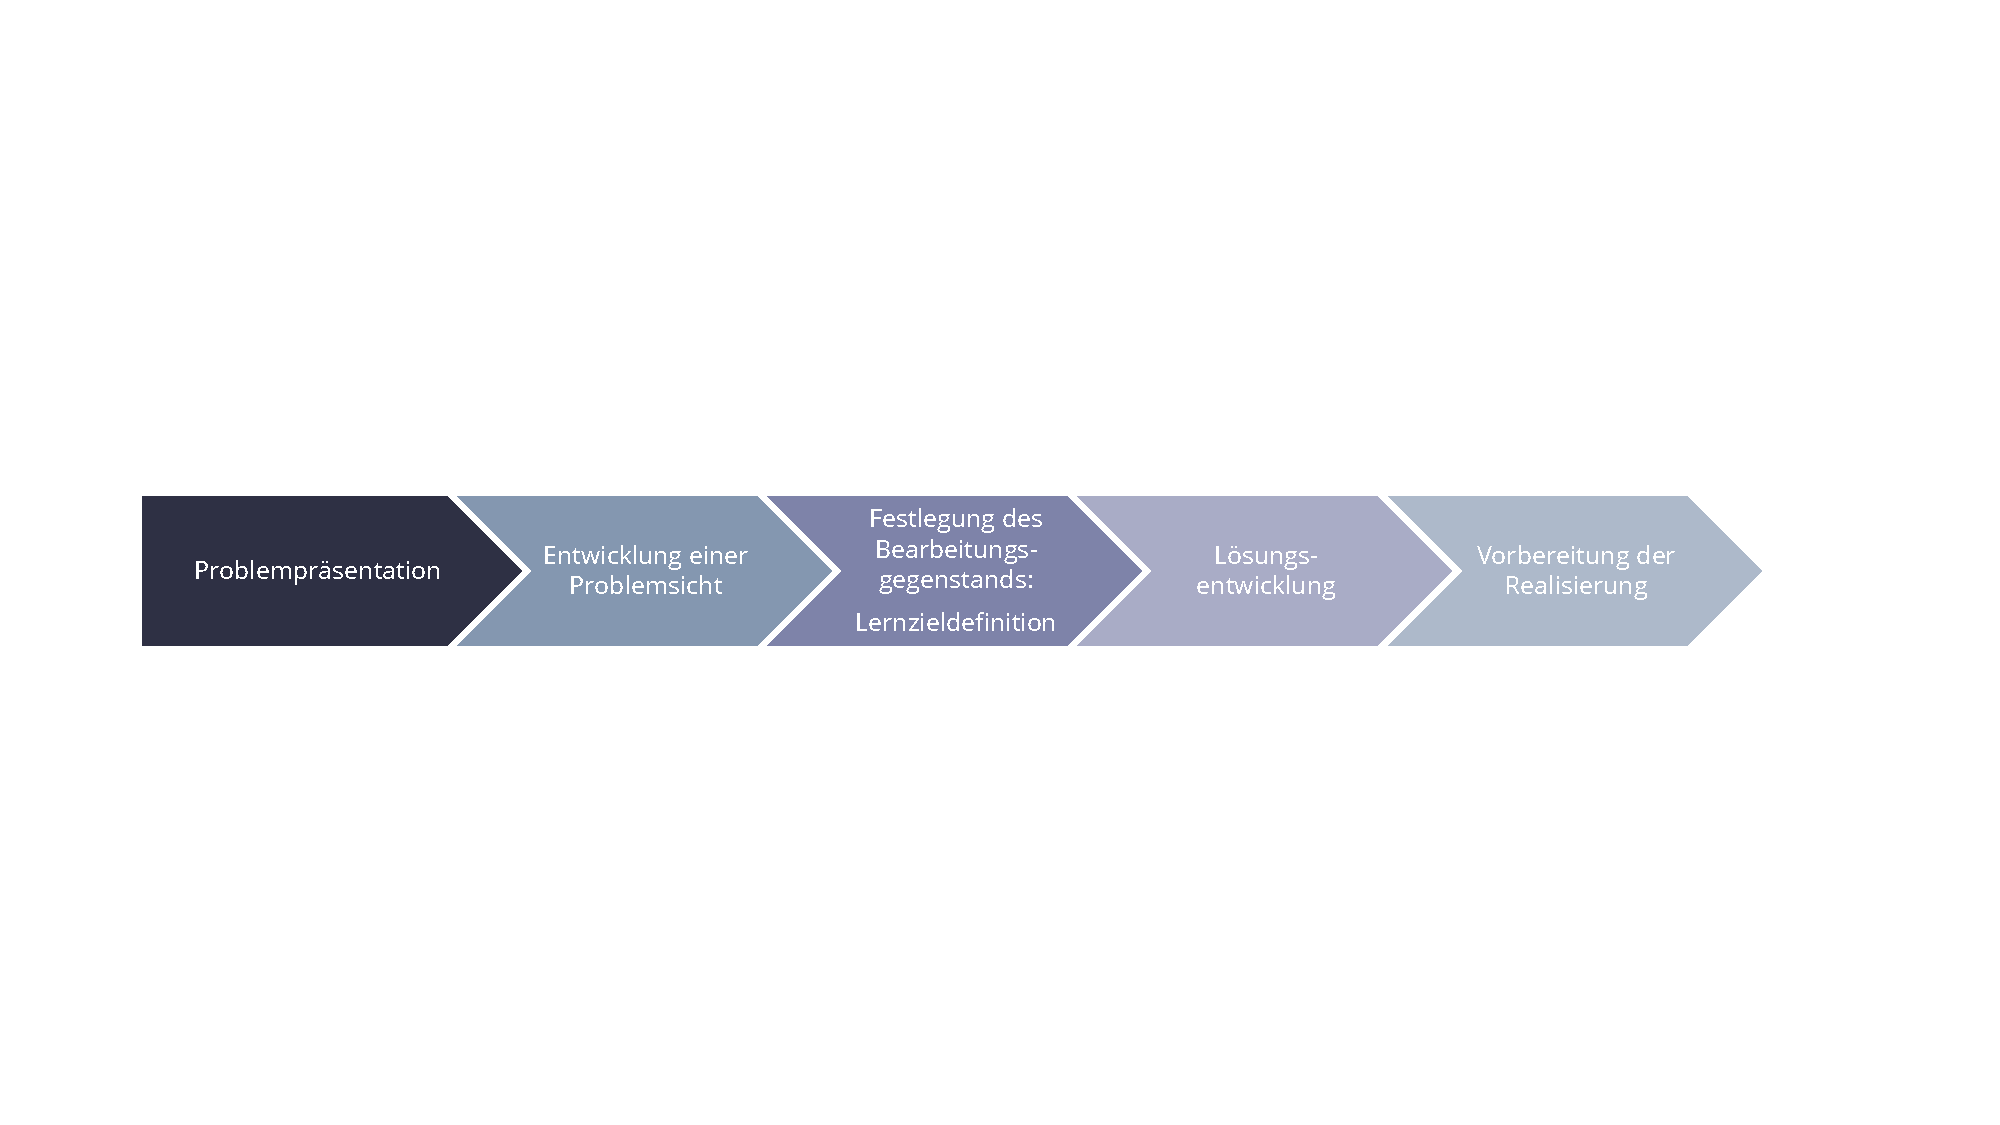
\includegraphics[width=\textwidth]{Grafiken/Beratungsablauf.pdf}
  \caption{Schematischer Ablauf einer Beratung (eigene Darstellung in Anlehnung an Kallmeyer (1985) zit. nach \textcite[179]{dinkelaker})}
  \label{fig:beratungsablauf}
\end{figure}

Die einzelnen Schritte der Beratung müssen allerdings nicht zwingend in dieser Reihenfolge stehen; in einem dynamischen Prozess wird es wahrscheinlich sein, dass einzelne Schritte übersprungen, zu einem späteren Zeitpunkt aufgegriffen oder erneut durchlaufen werden. Auch die Dauer der Beratungsphasen hängt stark vom Beratungsgegenstand und dem Setting ab (einmaliges Beratungsgespräch vs. Folge von Gesprächen z.B. über mehrere Wochen). \autoref{fig:beratungsablauf} zeigt diesen schematischen Ablauf eines Beratungsprozesses.

\subsection{Theoretische Beratungskonzeptionen}

Im medizinisch-pflegerischen Bereich haben sich einige Beratungsansätze als besonders wirkungsvoll erwiesen, die auf verschiedene Bezugswissenschaften wie Psychologie, soziale Arbeit und Pädagogik zurückgeführt werden können. Vier besonders weit verbreitete werden kurz beschrieben und Gemeinsamkeiten identifiziert, damit später nachvollziehbar wird, warum der personzentrierte Ansatz nach Carl Rogers für das geplante Angebot ausgewählt wird. Es ist dabei zu beachten, dass die Beratungsansätze nicht strikt voneinander getrennt zu sehen sind; sie enthalten einige verbindende Elemente, Übergänge können fließend bzw. je nach Bedarf wechselnd sein und sich ergänzen. Die Beschreibung der folgenden vier Konzepte basiert auf der Darstellung von \textcite[Kap. 8]{hacker2021}.

\paragraph{Kognitive Verhaltensberatung}

Dieser Ansatz zeichnet sich durch seinen Fokus auf gezielt beobachtbares Verhalten und dessen Veränderung aus. Er basiert auf Erkenntnissen der Lernpsychologie und hat zum Ziel, dysfunktionale Verhaltensweisen der ratsuchenden Person zu identifizieren und neue, hilfreichere Verhaltensmuster zu erlernen. Im Mittelpunkt der Beratung steht das Problem in der Gegenwart.

\paragraph{Systemische Beratung}

In der systemischen Sichtweise wird davon ausgegangen, dass jeder Mensch Teil verschiedener Systeme ist, z.B. eines Familiensystems. Probleme werden als Fehlfunktionen innerhalb eines Systems verstanden, um sie zu lösen müssen demnach Änderungen in der Konstellation des Systems vorgenommen werden. Systemische Berater:innen unterstützen hilfesuchende Personen beim Betrachten der Situation aus unterschiedlichen Perspektiven. Im Mittelpunkt der Beratung steht das System und alle, die daran beteiligt sind.

\paragraph{Lösungs- und ressourcenorientierte Beratung}

Dieser Ansatz hat zum Ziel, die Aufmerksamkeit möglichst schnell auf das Finden von Lösungen zu richten, damit Betroffene bald wieder in den gewohnten Alltag zurückkehren können. Es wird gemeinsam nach noch nicht bewussten Ressourcen und Lösungsideen gesucht. Demnach stehen die Ressourcen und Lösungsansätze im Mittelpunkt der Beratung.

\paragraph{Personzentrierte Beratung}
Der personzentrierte Ansatz versteht sich als ganzheitlich ausgerichtet und bemüht sich um ein Maximum an Respekt und Wertschätzung für das Individuum, seine Bedürfnisse und seine Autonomie. Der Blick der beratenden Person richtet sich besonders auf die Empfindungen, welche die ratsuchende Person in Bezug auf ihr Problem hat, und versucht diese empathisch zu verstehen. Ziel ist es, die ratsuchende Person auf dem Weg hin zu einer frei gewählten, auf ihre individuellen Bedürfnisse zugeschnittenen Lösung zu begleiten. Im Mittelpunkt steht die Person.

\paragraph{Gemeinsamkeiten dieser Beratungsansätze}

Allen geschilderten Beratungsansätzen ist gemeinsam, dass sie nicht versuchen, das Problem, seine Ursachen und Entstehungszusammenhänge in der Vergangenheit zu ergründen.\footnote{Der personzentrierte Ansatz lässt dies allerdings zu, wenn die ratsuchende Person den Wunsch danach äußert und selbst beginnt, die Zusammenhänge in der Vergangenheit zu untersuchen.} 
In allen genannten Beratungskonzeptionen zeichnet sich die beratende Person durch eine freundlich-zugewandte, nicht-wertende, nicht-urteilende Haltung aus. Diese besondere Art der respektvollen Haltung gegenüber den Klient:innen und ihren Problemen wurde aus dem personzentrierten Ansatz übernommen. Sie gilt als diejenige Haltung, die am wirksamsten dazu beiträgt, eine vertrauensvolle Beziehung zwischen den Beteiligten der Beratung herzustellen. Die Beziehung ist in allen genannten Ansätzen eine wichtige Basis für den Beratungserfolg. Darüber hinaus betonen alle aufgeführten Konzepte die Selbstverantwortlichkeit der ratsuchenden Person, die als einzige Expertin für ihr Problem angesehen wird; die beratende Person unterstützt diese bei der Suche nach der Problemlösung, stellt dafür ihr Wissen und ihren Beistand zur Verfügung; am Ende steht das sog. \textit{shared decision making}, eine gemeinsam erarbeitete und von den Klient:innen akzeptierte Lösung \autocite[127]{hacker2021}.

\subsection{Beratung und Lernen}

Was hat nun Beratung mit Lernen zu tun? Unter dem Punkt \textit{Festlegung des Beratungsgegenstands} wurde bereits gezeigt, dass das Defizit an Selbstbestimmung, das eine Person verspürt, dazu führen kann, dass sie beschließt, sich das notwendige Wissen aneignen zu wollen, um einer Situation dann kompetent begegnen zu können. \textquote[{\cite[187]{dinkelaker}}]{Beratung zielt insofern auf die Wiederherstellung fraglich gewordener Selbstbestimmung.} Die ratsuchende (erwachsene) Person wird als potentiell fähig zur Selbstbestimmung angesehen statt als erziehungsbedürftig. Das hierarchische Lehrkraft-Schüler:in-Beziehungsmodell verlagert sich hin zu einem Kommunikationsprozess auf Augenhöhe mit dem Ziel, Lernprozesse zu ermöglichen \autocite[vgl.][188]{dinkelaker}. Mollenhauer definierte schon Mitte der 60er Jahre drei Merkmale der Beratung \autocite[Mollenhauer 1965, zit.nach][189]{dinkelaker}:
\begin{itemize}
  \item Förderung von Selbsttätigkeit: eine eigene Antwort auf die Problemsituation finden, diese akzeptieren oder auch verwerfen dürfen
  \item Lebensnähe der in der Beratung vermittelten Informationen: direkter Bezug zur Problemlage der ratsuchenden Person
  \item Ermöglichung einer kritischen Reflexion der eigenen Lage aus einer Position der Distanz heraus
\end{itemize}

Die Merkmale Selbsttätigkeit, Lebensnähe und kritische Reflexion haben heute auch Eingang in den Unterricht bzw. in Bildungsveranstaltungen für alle Altersgruppen gefunden: Teilnehmenden- bzw. Schüler:innenorientierung, Handlungsorientierung und Selbstgesteuertes Lernen, lebensweltliche Bezüge und Bedeutsamkeit des Lernstoffs sowie die Förderung kritischer Reflexionsfähigkeit gehören zu den wichtigen Kennzeichen eines qualitativ hochwertigen Unterrichts \autocite[vgl.][Kap. 5.3]{hippel}.

\chapter{Der personzentrierte Ansatz nach C. Rogers}\label{chapter:rogers}

Bereits in der Einleitung dieser Arbeit wurde angesprochen, dass sich eine personzentrierte Herangehensweise an die Kommunikation mit Patient:innen schon seit vielen Jahren in der medizinischen Literatur finden lässt. In der Darstellung der verschiedenen Beratungskonzeptionen wurden wichtige Elemente erwähnt: Respekt vor der Autonomie jedes Menschen, eine wertschätzende und dabei nicht-wertende Haltung, empathisches Zuhören mit dem Fokus auf den Gefühlen. Im folgenden Kapitel wird nun der Entstehungszusammenhang des personzentrierten Ansatzes mit seinen wichtigsten theoretischen Grundzügen beschrieben. 

Am Ende dieses Abschnitts erfolgt der Versuch, aufzuzeigen, wie theoretische Strömungen aus Medizin, Pädagogik und Psychologie ineinander greifen können, um zu einer gemeinsamen \textquote{Philosophie} verbunden zu werden, die dem geplanten Angebot zu Grunde liegen soll.

\section{Entstehungszusammenhang}

Der personzentrierte Ansatz geht zurück auf den US-amerikanischen Psychologen, Wissenschaftler und (wenn auch in dieser Funktion bzw. Tätigkeit weniger bekannt) Pädagogen Carl Ransom Rogers (1902 - 1987). Eine besonders detailreiche Ausführung der Biographie von Carl Rogers, insbesondere mit Schwerpunkt auf seiner pädagogischen Tätigkeit, findet sich bei \textcite[vgl.][Kap. 3]{kunze}. 

Bereits während des Zweiten Weltkriegs begann er damit, die Beobachtungen, die er während seiner praktischen Arbeit als Erziehungsberater am \textit{Child Study Department of the Society for the Prevention of Cruelty to Children} gesammelt hatte, zu einem eigenen theoretischen Konstrukt auszuarbeiten. Er hatte 1931 am \textit{Teachers College} der Columbia-Universität promoviert und arbeitete in der Folgezeit dort als Dozent, wobei sein besonderes Interesse dem Verstehen von und dem Umgang mit Kindern aus problembelasteten, sozioökonomisch benachteiligten Elternhäusern galt. Ihm wurde zunehmend bewusst, dass seine Klient:innen bereits das Wissen darüber mitbrachten, welche Probleme und Erfahrungen für sie zentral waren und in welche Richtung der Weg zu deren Lösung führen müsste. 

Die entscheidende Frage, welche sein Schaffen über Jahrzehnte hinweg prägte, war: \textquote[{\cite[20]{weinberger}}]{Welche Bedingungen sind es, die dazu führen, dass eine Person von sich aus über ihr Erleben spricht, sich dabei besser verstehen lernt und schließlich zu Einstellungs- und Verhaltensänderung gelangt?}

1940 erhielt Carl Rogers eine Professur an der Ohio State University, ein Jahr später erschien sein Buch \textit{Counseling and Psychotherapy}, in welchem er erstmals die Methode der nicht-direktiven Beratung ausführte, welche später die Basis für den klientenzentrierten -- in der Weiterentwicklung dann personzentrierten -- Ansatz bildete.

In den späten Nachkriegsjahren (1957 bis 1963) konnte Rogers dann als Professor für Psychologie und Psychiatrie an der University of Wisconsin seine umfangreiche psychotherapeutische Forschungstätigkeit fortsetzen \autocite[vgl.][Kap. 5.2.1]{kunze}. Eine damals noch aufsehenerregende Neuheit auf diesem Gebiet war der systematische Einsatz von Tonbandaufzeichnungen, welche Rogers bereits seit den 1940er Jahren verwendete \autocite[239]{kunze}.

Rogers sah sich zu seiner Zeit, als die Psychoanalyse das therapeutische Denken und Handeln dominierte, heftiger Kritik ausgesetzt und war daher bestrebt, seinen Ansatz immer wieder auf den Prüfstand zu stellen. \textquote[{\cite[53]{rogers1977}}]{Keine andere therapeutische Richtung ist so gründlich mit den Methoden der empirischen Forschung untersucht worden wie die klientenzentrierte Psychotherapie}. Auch die neuere Psychotherapieforschung konnte viele Jahre später seinen Ansatz bestätigen (Orlinsky et al. 2004, S. 323, zit. nach \cite[21]{weinberger}). Die Forschungsergebnisse von Rogers und seinem Team haben bis heute sowohl inhaltlich als auch methodisch Vorbildcharakter und eine anhaltend \textquote{hohe Bedeutung} \autocite[239]{kunze}.

In späteren Jahren beschäftigten ihn die sogenannten Encounter-Gruppen\footnote{Zu Deutsch in etwa \textit{Begegnungsgruppen} -- hierunter wird eine besondere Form der personzentrierten Selbsterfahrung in der Gruppe verstanden.} sowie soziale und (friedens-)pädagogische Fragen. Anfang 1987 wurde er für den Friedensnobelpreis nominiert, er starb jedoch bereits am 04. Februar des selben Jahres in La Jolla, Kalifornien. Er gilt heute als einflussreicher Wegbereiter und Mitbegründer der Humanistischen Psychologie bzw. personzentrierten Gesprächspsychotherapie, der dritten großen Therapieform neben der Psychoanalyse und der Verhaltenstherapie \autocite[vgl.][24]{weinberger} bzw. des vierten großen Bezugssystems psychotherapeutischer Methoden neben Psychoanalyse, Lern- und Systemtheorie \autocite[892]{integrativePsycho}.

Als besonders bedeutsame Nachfolgende von Carl Rogers seien das Ehepaar Anne-Marie und Reinhard Tausch genannt, welche in der Nachkriegszeit die pädagogische Psychologie sowie die psychotherapeutische Ausbildung in Deutschland vorangebracht haben (\cite[vgl.][31]{weinberger}, \cite[vgl.][58]{kunze}), sowie der US-Amerikaner Marshall B. Rosenberg, welcher auf Basis von Rogers' personzentriertem Ansatz sein Konzept der Gewaltfreien Kommunikation entwickelte, welches bis heute weite Verbreitung findet \autocite[vgl.][58]{kunze}.

Zwar publizierte und forschte Rogers für die Pädagogik hauptsächlich aus psychologischer Perspektive, er verstand jedoch sich selbst auch immer als Pädagogen, vor allem in seiner Tätigkeit als Hochschullehrer. Er legte insgesamt wenig Wert auf die Abgrenzung zwischen Begrifflichkeiten und Fachgebieten \autocite[vgl.][17]{rogers1942}, sondern betonte stets die Gemeinsamkeiten und übergreifenden Prinzipien, die seiner Erkenntnis nach zum Erfolg führten. Psychologie und Pädagogik lagen für ihn so nah beieinander, dass sich in vielen seiner zentralen Werke sowohl Kapitel zum Thema Psychotherapie als auch zum Thema Pädagogik und Lernen finden. 

So widmete er 1961 dem Thema Lehren und Lernen in seinem Buch \textit{Entwicklung der Persönlichkeit. Psychotherapie aus der Sicht eines Therapeuten}\footnote{Englischer Originaltitel: \textit{On Becoming a Person. A Therapist's View of Psychotherapy} Boston 1961} ein umfangreiches Kapitel, ebenso schon 1951 in \textit{Die klientenzentrierte Gesprächspsychotherapie}\footnote{Englischer Originaltitel: \textit{Client-Centered Therapy} Boston 1951} ein Kapitel mit dem Titel \textit{Schüler-bezogenes Unterrichten}. Sein wichtigstes Werk in Bezug auf die praktischen Implikationen seiner Theorien auf die Pädagogik dürfte \textit{Lernen in Freiheit. Zur Bildungsreform in Schule und Universität}\footnote{Englischer Originaltitel: \textit{Freedom to learn. A view of what education might become.} Columbus/Ohio 1961} von 1969 sein.  Er formuliert darin seine Überzeugungen sehr klar: \textquote[{\cite[104]{rogersLernenFreiheit}}]{Und zwar glaube ich schlicht, daß Lehren eine weitgehend überschätzte Tätigkeit ist.} Statt erfolglos zu versuchen, Menschen etwas zu lehren, baue er \textquote[{\cite[9]{rogersLernenFreiheit}}]{auf die Entwicklungsmöglichkeit und die Weisheit des Menschen}. Lehrpersonen sollten sich als \textit{Facilitators} (zu dt. etwa Ermöglichende) begreifen, die die Bedingungen für gutes Lernen herstellten, denn: \textquote[{\cite[105]{rogersLernenFreiheit}}]{Der einzige Mensch, den man gebildet nennen kann, ist jener, der gelernt hat, wie man lernt}.

\section{Menschenbild und zentrale theoretische Elemente}

Carl Rogers gehört wie erwähnt zu den Begründern der Humanistischen Psychologie und war davon überzeugt, dass in jedem Menschen von Geburt an das Bestreben angelegt ist, sich konstruktiv weiterzuentwickeln, seine Persönlichkeit zu entfalten und sich selbst zu verwirklichen. Anders als Psychoanalyse und Behaviorismus, die von einer Determination des Menschen durch das Unbewusste bzw. durch äußere Reizbedingungen ausgehen \autocite[vgl.][35]{weinberger}, betont Rogers die menschliche Individualität und Freiheit. Um sein theoretisches Konzept verständlich zu machen werden einige zentrale Begriffe, die Rogers geprägt hat, im Folgenden kurz erläutert.

\subsection{Theoretische Grundannahmen}
\paragraph{Aktualisierungstendenz} Sie bezeichnet jene im Menschen angelegte, grundsätzliche Fähigkeit zu Entwicklung und innerem Wachstum, welche immer in diejenige Richtung führt, die dem Erhalt des Menschen in seiner psychischen und physischen Einheit am meisten dienlich ist. Die Aktualisierungstendenz ist somit \textquote[{\cite[24]{weinberger}}]{das grundlegende Axiom} der personzentrierten Haltung, welche in ihrem gesamten Handeln darauf ausgelegt ist, diese  \textquote[{\cite[41]{rogers1977}}]{inhärente Tendenz zur Entfaltung aller Kräfte} zu unterstützen. \textquote[{\cite[41]{rogers1977}}]{Wenn diese Tendenz nicht behindert wird, bewirkt sie verläßlich beim Individuum Wachstum, Reife und eine Bereicherung des Lebens}.

\paragraph{Selbstkonzept} Im Laufe des Heranwachsens beginnt der Mensch, ein Selbstkonzept auszubilden. Es basiert auf der Qualität der zwischenmenschlichen Beziehungen, welche ein Kind in seinem Umfeld erfährt. \textquote[{\cite[42]{rogers1977}}]{Man kann es sich als eine strukturierte, konsistente Vorstellungsgestalt denken, die sich zusammensetzt aus den Wahrnehmungen vom \textquote{Ich} oder \textquote{Mich} und den Wahrnehmungen von den Beziehungen dieses \textquote{Ich} zur Außenwelt und zu anderen Personen}. 

\paragraph{Selbstaktualisierungstendenz} Sie entwickelt sich als Teil innerhalb der Aktualisierungstendenz. Erfahrungen werden mit zunehmendem Alter der Heranwachsenden nicht mehr nur noch entsprechend dem unmittelbaren körperlichen Erleben (in Rogers' Worten: der organismischen Bewertung), sondern auch danach beurteilt, ob sie das Selbstkonzept aufrecht erhalten. Die Selbstaktualisierungstendenz ist eine starke Macht: Ihr wird in innerpsychischen, unbewusst ablaufenden Prozessen häufig der Vorzug vor der organismischen Bewertung eingeräumt, um das Konstrukt des Selbstkonzepts nicht zu gefährden. \textquote[{\cite[140]{rogers1977}}]{Das Individuum neigt dazu, seinen eigenen Erfahrungsprozeß zu ignorieren, sobald er mit diesen Konstrukten in Konflikt gerät. Es versucht, anders gesagt, das Selbst zu sein, das andere von ihm erwarten, anstelle des Selbst, das es eigentlich ist.}

\paragraph{Inkongruenz} Wenn Menschen Erfahrungen machen, deren organismische Bewertung nicht mit dem Selbstkonzept in Übereinstimmung gebracht werden kann, entsteht ein Zustand der Inkongruenz, also der Unvereinbarkeit der beiden Tendenzen zur Aufrechterhaltung und Entfaltung des menschlichen Organismus (also dessen psychischer und physischer Gesamtheit) und der Tendenz zum Schutz des Selbstkonzepts. Rogers definiert Inkongruenz als \textquote[{\cite[43]{rogers1977}}]{Diskrepanz zwischen dem Erleben des Organismus und dem bewußten Selbstkonzept.} \textquote[{\cite[28]{weinberger}}]{Aus dieser Unvereinbarkeit resultieren Spannungen, die die Person löst, indem [sie] die Erfahrungen entweder verzerrt, d.h. verfälscht, wahrnimmt oder ganz verleugnet}. 

\begin{beispiel}
  Dieses Beispiel ist angelehnt an \textcite[26]{weinberger}: Ein Kind wird von den Eltern mit der Haltung konfrontiert, dass Schmerzen nicht gezeigt, ja eigentlich gar nicht gefühlt werden dürfen, da dies ein Zeichen von Schwäche sei: \textquote{Ein Indianer kennt keinen Schmerz!}. Es entwickelt dementsprechend ein Selbstkonzept in enger Anlehnung an diese Bewertungen der Bezugspersonen. Wenn das Kind Schmerzen erlebt, entsteht eine Inkongruenz: Die organismische Bewertung stuft den Schmerz als unangenehmes Gefühl ein, welches z.B. über Weinen ausgedrückt werden will. Die Selbstaktualisierungstendenz wirkt dem jedoch entgegen und hält das Selbstkonzept aufrecht, welches es unmöglich macht, diesen Schmerz nach außen zu zeigen: \textquote{Ich bin stark, ich bin nicht weinerlich.} Es kommt entweder zu einer Verleugnung (\textquote{Es hat gar nicht weh getan.}) oder zu einer Verzerrung der Schmerzerfahrung (\textquote{Mir macht das nichts aus.}). Es entsteht somit ein innerpsychischer Spannungszustand.
\end{beispiel}

\subsection{Bedingungen des therapeutischen Prozesses}

Carl Rogers formulierte in vielen seiner Publikationen die zentralen Bedingungen für Therapie und Lernen, beispielsweise in \textquote[{\cite[46-49]{rogers2020theorie}}]{\textit{Eine Theorie der Psychotherapie, der Persönlichkeit und der zwischenmenschlichen Beziehungen}}, \textquote[{\cite[Kap. VI.14]{rogers1961}}]{\textit{Entwicklung der Persönlichkeit}} oder in \textquote[{\cite[149-165]{rogers1977}}]{\textit{Therapeut und Klient}}. Sie werden im Folgenden überblicksartig vorgestellt. 

\paragraph{Kongruenz} Carl Rogers vertrat den Standpunkt, dass die Kongruenz der beratenden Person das wichtigste der drei Elemente einer gelingenden Beratung bzw. Therapie sei, noch vor empathischem Verstehen und unbedingter Wertschätzung (s.u.) \autocite[vgl.][162]{rogers1977}.
 Dieses wichtige Merkmal der Therapie bzw. Beratung bezieht sich ganz auf die beratende Person. Sie soll sich nicht verstellen, sondern als echter Mensch mit eigenen Gefühlen anwesend sein und es der ratsuchenden Person auf diese Weise ermöglichen, Vertrauen aufzubauen und die unbedingte Wertschätzung auch anzunehmen \autocite[vgl.][151]{rogers1977}.

\paragraph{Empathisches Verstehen} Empathisches Zuhören und Verstehen meint, sich ganz und gar auf die Empfindungen einer Person einzustellen, diese möglichst genau wahrzunehmen und innerhalb des Wertesystems dieser Person nachzuvollziehen. Ein empathisch verstehender Mensch enthält sich aller eigenen Bewertungen, äußert keine Kritik und keine Ratschläge. Stattdessen gibt er mit eigenen Worten wider, was er verstanden hat. \textquote[{\cite[216]{rogers1977}}]{Die innere Welt des Klienten mit ihren ganz persönlichen Bedeutungen so zu verspüren, als wäre sie die eigene (doch ohne die Qualität des \textquote{als ob} zu verlieren), das ist Empathie}. In dieser intensiven Art der Kommunikation werden Gesprächspartner:innen \textquote[{\cite[41]{weinberger}}]{ständig angeregt, sich mit den mit ihrem Erleben verbundenen Gefühlen und Empfindungen auseinander zu setzen und durch ein Abwägen, Differenzieren und Konkretisieren ihrer Wünsche und Ziele schrittweise zu einer Klärung ihrer inneren und äußeren Konflikte zu kommen}.

\paragraph{Unbedingte Wertschätzung} Einer Person unbedingte Wertschätzung entgegen bringen bedeutet, klar zu trennen zwischen den eigenen Bewertungen des Verhaltens bzw. der Einstellungen dieser Person und ihrem Wert \textit{als} Person. \textquote[{\cite[59]{weinberger}}]{Es geht darum, den anderen in seinem \textquote{Da-Sein} zu akzeptieren, ohne diese Akzeptanz an Bedingungen zu knüpfen}. Berater:innen erfüllen auf diese Weise das wichtige menschliche Grundbedürfnis nach unbedingter Anerkennung, welches von Rogers als eines der zentralen Elemente in der gelungenen Erziehung von Kindern genannt wird. Dabei darf Anerkennung nicht mit Zustimmung verwechselt werden: \textquote[{\cite[46]{rogers1942}}]{Der Berater akzeptiert und anerkennt die positiven Gefühle, die ausgedrückt werden, auf die gleiche Art, in der er die negativen Gefühle akzeptiert und anerkannt hat. [Auch] [d]iese positiven Gefühle werden nicht mit Beifall oder Lob akzeptiert. Moralische Werte gehen in diese Art der Therapie nicht ein.} Es handelt sich also um eine nicht-wertende Art der Anerkennung, im Sinne eines \textit{Erkennens}, dass diese Gefühle in diesem Menschen vorhanden sind, ganz gleich, welcher Art sie sein mögen. Oder, mit Rogers' Worten: \textquote[{\cite[Hervorh. im Orig.][155]{rogers1977}}]{Ich akzeptiere das, was \textit{ist}}.

\paragraph{Selbstempathie und Selbstexploration} Wichtige Grundlage, um Klient:innen diese Erkundung des eigenen Fühlens und Erlebens, genannt \textit{Selbstexploration}, zu ermöglichen und dabei kongruent als Person zugegen zu sein, ist die \textit{Selbstempathie} auf 
Seiten der beratenden Person, also die intensive Wahrnehmung und Auseinandersetzung mit den eigenen Gefühlen. \textquote[{\cite[214]{rogers1977}}]{Wirklich zu sein schließt die für den Therapeuten schwierige Aufgabe mit ein, mit dem Fließen des eigenen Erlebens vertraut zu sein, diesem Fließen, das besonders durch seine Vielschichtigkeit und seinen ständigen Wandel gekennzeichnet ist.}

\subsection{Der zentrale Stellenwert der Beziehung in Therapie und Pädagogik}
Rogers war der Ansicht, dass die genannten Bedingungen für einen gelingenden therapeutischen Prozess ausreichend waren: Sobald zwischen Therapeut:innen und Klient:innen ein zwischenmenschlicher Kontakt hergestellt war, der von Kongruenz, empathischem Verstehen und unbedingter Wertschätzung auf Seiten der Therapeut:innen geprägt war, entsteht eine \textquote[{\cite[47]{rogers2020theorie}}]{echte Beziehung zweier Personen}. \textquote[{\cite[892]{integrativePsycho}}]{Die zentrale Bedeutung der Qualität der Beziehung zwischen Patient und Therapeut - inklusive einer empathischen Haltung} zählt heute zu den übergeordneten Prinzipien, \textquote[{\cite[892]{integrativePsycho}}]{über die in allen psychotherapeutischen Schulen/Methoden Einigkeit besteht}. Eine Verknüpfung dieser besonderen Art der Beziehung zum Thema Lernen und der hohe Stellenwert, den Rogers ihr beimaß, findet sich später in seinen Ausführungen zur Ermöglichung eines \textquote{Lernen[s] in Freiheit} wieder: \textquote[{\cite[107]{rogersLernenFreiheit}}]{Die Förderung signifikanten Lernens hängt von bestimmten einstellungsbedingten Qualitäten ab, die in der persönlichen Beziehung zwischen dem Facilitator und dem Lernenden existieren.}. Auch für Lehrende im Sinne Rogers' - er bezeichnete sie als \textit{facilitators}, um die Abgrenzung von den Lehrenden zu betonen, die die herkömmliche, direktive Haltung vertraten -  seien also das \textquote{Real-sein}, \textquote{Wertschätzung, Anerkennung, Vertrauen} sowie \textquote{einfühlendes Verständnis} die wichtigsten Merkmale im Kontakt mit den Lernenden \autocite[107-114]{rogersLernenFreiheit}. Die persönliche therapeutische oder pädagogische Beziehung bildet demnach den Ausgangspunkt für erfolgreiche Weiterentwicklung und signifikantes, d.h. dauerhaftes, der Entfaltung dienliches, Lernen. Dieses signifikante Lernen findet nach Rogers' Ansicht in Therapie und Erziehung gleichermaßen statt und basiert auf denselben wichtigen Grundbedingungen -- er beschreibt dies ausführlich beispielsweise im Kapitel \textit{Signifikantes  Lernen: In Therapie und Erziehung} in seinem Buch \textit{Entwicklung der Persönlichkeit} \autocite[273-289]{rogers1961}. 

\chapter{Den ganzen Menschen sehen - in Medizin, Psychologie und Pädagogik}

Es stellt sich nun die Frage, wie zu Gunsten eines schmerzkranken Menschen eine Verbindung hergestellt werden kann zwischen den drei großen Domänen, in deren Mittelpunkt er sich befindet: Medizin, Psychologie und (Erwachsenen-)Pädagogik. Auf den ersten Blick mag es sich um Lebensbereiche handeln, die weitgehend getrennt voneinander praktiziert und erforscht werden, doch es finden sich bei allen drei Fächern Ansätze und Theorien, die in ihrem Kern auf eine ähnliche philosophische Grundlage bzw. ein bestimmtes Menschenbild zurückgeführt werden können. Diese daraus hervorgehende verbindende Philosophie für das geplante Angebot kann folgendermaßen auf den Punkt gebracht werden:

\begin{displayquote}\normalfont
  Der Mensch ist nicht das Objekt einer von außen kommenden Belehrung oder Heilung. Die Kräfte zur Entfaltung, Ganz-werdung, Entwicklung seines Selbst und Aneignung von Wissen und Können liegen \textit{in ihm}.
\end{displayquote}

\section{Medizin: Ganzheitlichkeit, biopsychosoziales Modell, Resilienz} 

In der Medizin wird dieses Bestreben, den Menschen als Einheit wahrzunehmen und seine Autonomie hervorzuheben, in der zunehmenden Verbreitung sogenannter \textbf{integrativer Ansätze} sichtbar. \textquote[{\cite[16]{integrativeMedizin}}]{Integrative Medizin bedeutet das Zusammenführen jahrtausendealter ganzheitsmedizinischer Gesundheitssysteme mit der auf der klassischen Naturwissenschaft gegründeten konventionellen Schulmedizin.}\footnote{Dabei fließen etablierte Verfahren wie Physio- und Psychotherapie, Entspannungsverfahren, Biofeedback und Ähnliches ebenso ein wie umstrittenere Gebiete, beispielsweise Homöopathie, Anthroposophische, Traditionelle Chinesische und Kneipp-Medizin.  Die Forderungen der Integrativen Medizin zum Umdenken im Gesundheitssystem gehen zum Teil sehr weit und haben eine grundlegende Veränderung des herkömmlichen medizinischen Weltbilds vor Augen.} Für das Vorhaben, ein personzentriertes Psychoedukations- und Beratungsangebot für Schmerzpatient:innen zu entwickeln, ist der entscheidende Aspekt der Ganzheitsmedizin, dass sie die Ganzheitlichkeit des Organismus bewusst machen will; statt den menschlichen Körper in Organsysteme aufzuteilen und diese getrennt voneinander zu behandeln strebt die ganzheitliche Medizin an, eine Person als Einheit von Körper, Geist und Seele zu sehen und bevorzugt daher Behandlungsmethoden, welche sich auf den Menschen als Ganzes auswirken. \textquote[{\cite[339]{HeftSchmerz5}}]{Als ganzer Mensch in all seinen Dimensionen gesehen, anerkannt und behandelt zu werden, ist ein zentraler Aspekt der therapeutischen Beziehung und nicht nur eine Beigabe.} Insbesondere in der Behandlung von chronisch Schmerzkranken ist lange bekannt, dass eine rein medikamentöse und/oder operative Behandlung nicht ausreichend ist. \textquote[{\cite[16]{integrativeMedizin}}]{Eine moderne Medizin muss ihr Credo grundlegend ändern: Ganzheit leben statt Teile des Körpers reparieren.} Eines der international wichtigsten und allgemein anerkannten Krankheitsmodelle, das \textbf{Biopsychosoziale Modell von Gesundheit und Krankheit} wurde Ende der 1970er Jahre von George Engel aufgestellt.
\begin{displayquote}[{\cite{Biopsychosozial}}][]
  [Dieses Modell] geht von einem integrativen medizinischen Ansatz aus, der Krankheit nicht rein mechanistisch, sondern als Störung der Interaktion von körperlichen, psychischen und sozialen Faktoren versteht. Biologische, psychische und soziale Faktoren sind folglich nicht eigenständig, sondern sind Teile eines verflochtenen Ganzen;  deren dynamische Wechselbeziehungen von kausaler Bedeutung für die Entstehung und den Verlauf von Krankheiten sind. So gilt es bei Prävention, Diagnostik, Behandlung und Rehabilitation von Krankheiten nicht nur biologische Faktoren (z.B. genetische Merkmale) zu berücksichtigen, sondern auch die soziokulturellen (z.B. Schichtzugehörigkeit) und psychologischen (z.B. Copingstrategien) Merkmale von Patienten mit einzubeziehen.
\end{displayquote}

Dieses Modell ist hilfreich, um sich darüber klar zu werden, dass die Begriffe \textquote{krank} vs. \textquote{gesund} im Sprachgebrauch meistens als Dichotomie, als entweder-oder, verwendet werden. Wer krank ist, kann nicht gleichzeitig gesund sein und umgekehrt. \textquote[{\cite[16]{knuf}}]{Eine solche Vorstellung von Gesundheit und Krankheit deckt sich nicht mit der Wirklichkeit und sie ist obendrein inhuman}. Vorgeschlagen wird daher, Gesundheit und Krankheit als zwei Enden eines Kontinuums zu betrachten; jeder Mensch befindet sich zu jedem Zeitpunkt seines Lebens irgendwo zwischen diesen beiden Polen, trägt also gesunde und kranke Anteile in sich. Diese Sichtweise ermöglicht es professionell Tätigen ebenso wie Patient:innen, den Blick zu weiten und die Ressourcen, die jeder Mensch mitbringt, zu erkennen \autocite[17]{knuf}. Diese Ressourcen kann ein Mensch dann nutzen, um sich dem \textquote{gesunden} Pol anzunähern.

Bekannt geworden ist in diesem Zusammenhang auch die \textbf{Resilienzforschung}, die eng mit dem Konzept der Salutogenese verbunden ist \autocite[vgl.][174]{integrativJakesz}. Dieses Forschungsgebiet befindet sich im Schnittbereich zwischen Medizin und Psychologie. Die zentrale Frage lautet: Was ist es, das Menschen gesund erhält? Beide Konzepte, Salutogenese und Resilienz, wenden den Blick ins Innere; auf die Ressourcen, die dort in jedem Menschen angelegt sind. Jakesz definiert Resilienz als \textquote[{\cite[174]{integrativJakesz}}]{eine dem Menschen innewohnende Bereitschaft, die ihn stimuliert zu leben und das Leben zu erhalten.} Physische und psychische Widerstandsfähigkeit speisen sich demnach aus einer akzeptierenden, liebevollen Haltung dem eigenen Ich gegenüber, dem Vertrauen auf die eigenen Fähigkeiten zur Bewältigung von Herausforderungen sowie - und hier findet ein Übergang in die spirituelle Dimension statt - der Auseinandersetzung mit der Sinnfrage des eigenen Lebens und dem Erreichen eines inneren Friedens im Sinne eines mit sich selbst in Einklang und Übereinstimmung Kommens. \textquote[{\cite[176]{integrativJakesz}}]{Dieser Frieden wird bewirkt durch ein Herausgehen aus der Energie der Verurteilung, Beurteilung und des Wertens und ein Hineintreten in einen Status der Beobachtung, der liebevollen Betrachtung und des wertfreien Wahrnehmens}. 

Aus Sicht einer ganzheitlich orientierten, dem bio-psycho-sozialen Modell verpflichteten Medizin können alle im medizinisch-pflegerischen Bereich Tätigen ihre Patient:innen beratend unterstützen, doch die Verantwortung für diesen Prozess der Aktivierung der Selbstheilungskräfte liegt nicht bei Ärzt:innen oder Heiler:innen im weiteren Sinne, sondern ganz und gar beim gesund-bleiben- oder gesund-werden-wollenden Individuum selbst. 


\section{Psychologie und Erwachsenenpädagogik: Personzentrierung und Ermöglichungsdidaktik} In der Auseinandersetzung mit dem von Carl Rogers entwickelten Personzentrierten Ansatz wurde bereits deutlich, dass auch für Rogers die Eigenverantwortlichkeit des Einzelnen sowie das wertungsfreie Annehmen der Klient:innen, ebenso wie der eigenen Person, eine zentrale Rolle spielt. Er war überzeugt davon, dass keine von außen kommende Interpretation und kein Ratschlag die Probleme eines Menschen lösen können. Die Hinwendung nach Innen, in Richtung des Erkennens und Akzeptierens der eigenen Gedanken und Gefühle, ebnet den Weg \textquote[{\cite[182]{rogers1942}}]{zu der tiefsten aller Einsichten, daß nämlich die Kräfte, die [eine] Entscheidung treffen werden, in ihm selbst liegen, daß er selbst die Fähigkeit zum Wachsen und zur Unabhängigkeit besitzt.}

 Rogers widmete sich der Thematik Lehren und Lernen ausführlich und konstatierte: \textquote[{\cite[271]{rogers1961}}]{Ich selbst bin zu der Überzeugung gelangt, daß das einzige das Verhalten signifikant beeinflussende Lernen das Lernen durch Selbst-Entdecken und Selbst-Aneignen ist.}  Hier schließt sich der Kreis: Folgt man der Denktradition des Konstruktivismus, die davon ausgeht, \textquote[{\cite[64]{hippel}}]{dass wir über die Welt kein objektives Wissen haben können, sondern nur über subjektive Konstruktionen verfügen}, so ist die logische Konsequenz für das pädagogische Selbstverständnis und für die Didaktik, dass Lernen nicht erzwungen werden kann. Statt einem Eintrichtern von als objektiv wertvoll betrachteten Lerninhalten werden \textquote[{\cite[64]{hippel}}]{Deutungsangebote} gemacht; die Verantwortung für das eigene Lernen liegt beim Lernenden. Rogers betonte immer wieder die dem Menschen innewohnende Kraft, die ihn stetig antreibt, sich zu entfalten und weiterzuentwickeln, also neugierig zu sein, zu lernen und diesen Lernprozess für sich selbst passend zu steuern \autocite[vgl.][157]{rogersLernenFreiheit}. Diese Haltung taucht auch in der jüngeren pädagogischen Literatur wieder auf, zum Beispiel als \textquote[{\cite[48]{arnold}}]{Mündigkeit des Lerners}. \textquote[{\cite[45]{arnold}}]{[Die Berufs- und Erwachsenenpädagogik] beginnt zu verstehen, dass Lernen nicht \textquote{vermittelt}, sondern lediglich ermöglicht und gefördert werden kann}. 

Die Lehrkraft wird dementsprechend als  Person betrachtet, deren Aufgabe die Ermöglichung des Lernens ist, die also ein Setting herstellt, welches Lernangebote bereit hält. Lehrkräfte haben dann \textquote[{\cite[45]{arnold}}]{eine andere Art von Verantwortung, die ihren professionellen Ausdruck stärker in einer Lernberatung als im Lehren oder gar Vermitteln(wollen) findet.}  Diese \textquote{Ermöglichungsdidaktik}, ein von \citeauthor{arnold} geprägter Begriff, hat viele Überschneidungspunkte mit der personzentrierten Erwachsenenpädagogik, wie \citeauthor{kunze} sie beschreibt. Sie hat sich intensiv damit auseinandergesetzt, Rogers' personzentrierten Ansatz in die pädagogische Arbeit zu überführen \autocite[Kap. 5]{kunze}. Diese Form der Pädagogik legt \textquote[{\cite[161]{kunze}}]{den Fokus konsequent auf potenzielle Selbstbestimmung, Selbstaneignung und selbstentdeckendes Lernen, was nicht mit Strukturlosigkeit zu verwechseln ist und auch nicht bedeutet, dass eine Seminarleitung ihre personalen, fachlichen und erwachsenenpädagogischen Kompetenzen nicht zur Verfügung stellen würde.} Dozent:innen sollen sich demnach als \textit{facilitators} verstehen und eine Haltung verinnerlichen, die die Aktualisierungstendenz und die organismischen Bewertungen der Teilnehmenden wahr- und ernst nimmt; dies setzt auch ein Vertrauen der \textit{facilitators} in die Lernenden voraus \autocite[vgl.][281]{kunze}. 

\begin{praxis}
  Dem geplanten Angebot soll insgesamt eine Haltung den Teilnehmenden gegenüber zu Grunde liegen, die ihnen die Verantwortung für den eigenen Lernprozess lässt und auf ihre ihnen innewohnenden Kräfte zur Entfaltung und Gesund-werdung (Resilienz) vertraut. Dozent:innen des Angebots sollen sich als \textit{facilitators} begreifen und individuelle Lernarrangements herstellen, die den Lernenden signifikantes Lernen ermöglichen. 
\end{praxis} 


\begin{figure}
  \centering
  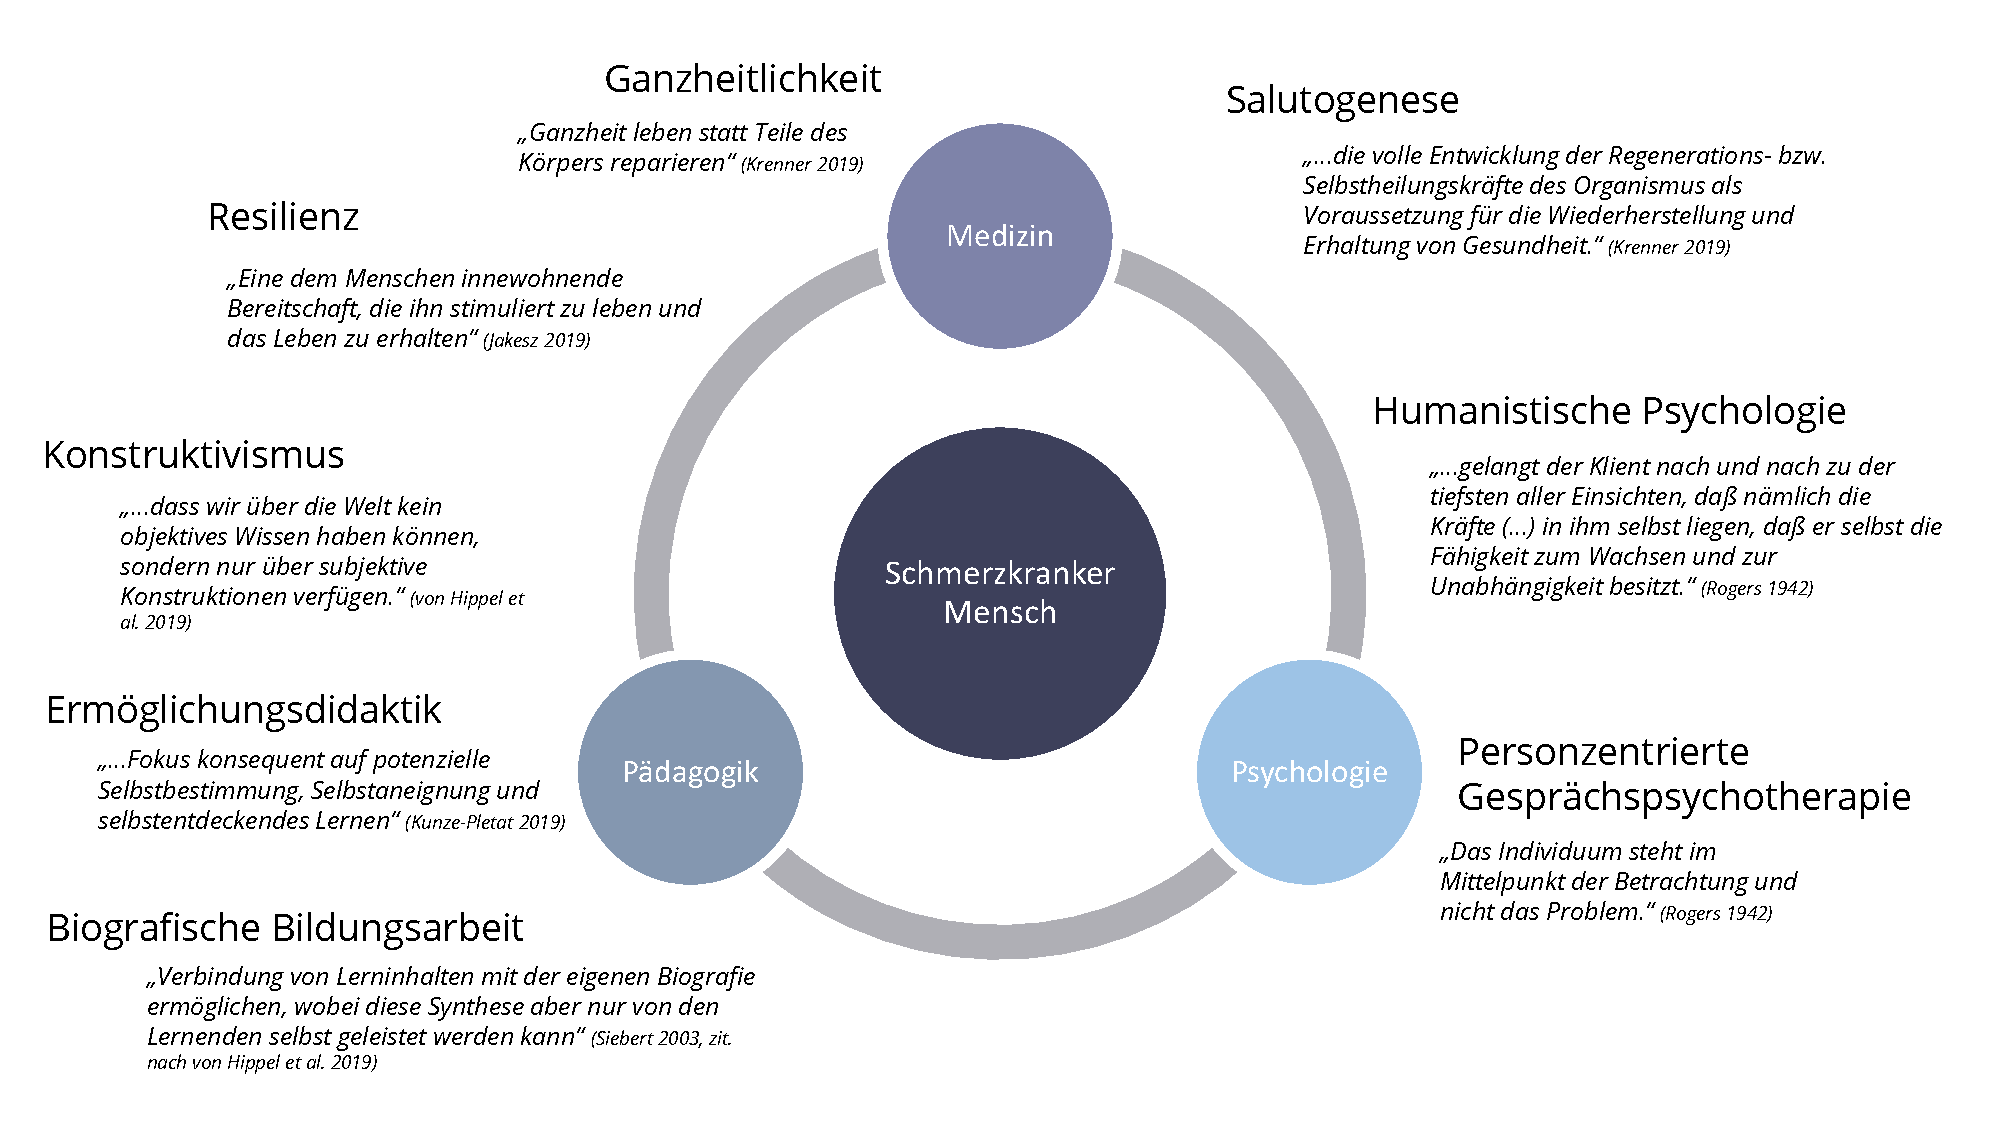
\includegraphics[width=1.1\textwidth]{Grafiken/Der Schmerzkranke im Mittelpunkt.pdf}
  \caption{Der schmerzkranke Mensch im Mittelpunkt (eigene Darstellung)}
  \label{fig:schmerzmensch}
\end{figure}

\autoref{fig:schmerzmensch} verdeutlicht, wie die ganzheitliche Medizin (und innerhalb dieser insbesondere das Konzept der Resilienz), der personzentrierte Ansatz der Humanistischen Psychologie und bestimmte Strömungen der Pädagogik bzw. Didaktik (darunter vor allem die konstruktivistische, identitätstheoretische und subjektorientierte Didaktik) miteinander in Verbindung gebracht werden. Sie alle betonen die Eigenverantwortung eines jeden Individuums zur eigenen Gesundheit, zur Persönlichkeitsentwicklung und zum Lernen; sie lehnen eine paternalistische Einstellung professioneller Helfender ab und vertreten eine Haltung, die durch höchsten Respekt für die körperliche, geistige und seelische Integrität eines jeden Menschen gekennzeichnet ist. 

\chapter{Bedarfsermittlung und Angebotsentwicklung}

Es steht nun fest, auf welche theoretische Basis die Angebotsidee aufbauen soll und es erfolgte eine entsprechende Auseinandersetzung mit den zentralen Begrifflichkeiten und deren inhaltlicher Definition. Zudem wurden in den Fachgebieten Medizin, Psychologie und Pädagogik diejenigen Strömungen identifiziert, welche sich logisch und stimmig miteinander zu einem wissenschaftlich begründbaren Gesamtkonzept verbinden lassen.

Bis zu diesem Zeitpunkt handelt es sich noch immer lediglich um eine ausführlich überlegte Angebotsidee; bis zur tatsächlichen Realisierung ist es noch ein weiter Weg. Daher erfolgt in der nächsten Phase eine Auseinandersetzung mit den einzelnen Schritten des Angebotsplanungsprozesses. Bevor die Planung beginnt werden zunächst wieder einige zentrale Begriffe definiert und Überlegungen darüber angestellt, wie Informationen über den Bildungsbedarf der Zielgruppe erhoben werden können.

\section{Programm und Angebot} Während die Begriffe Angebot und Programm im alltäglichen Sprachgebrauch häufig synonym genutzt werden, wenn von Bildungsdienstleistern wie beispielsweise einer Volkshochschule die Rede ist, müssen diese Begriffe für die Verwendung in bildungswissenschaftlichen Zusammenhängen genau unterschieden werden, um sie als \textquote[{\cite[27]{fleige}}]{übergreifende Strukturprinzipien in der Erwachsenen- und Weiterbildung} verstehen zu können. Vereinfacht gesagt setzt sich das \textbf{Programm} aus der Gesamtheit aller Angebote zusammen. Die Programmgestaltung gehört zu den übergeordneten Aufgaben der Mitarbeitenden in Erwachsenenbildungseinrichtungen. Im Programm einer Institution bildet sich zum Beispiel deren bildungstheoretische Ausrichtung ab, spezifische inhaltliche, aber auch lernkulturelle Schwerpunkte der Einrichtung werden anhand des Programms erkennbar. Das \textbf{Angebot} beschreibt auf der Mikro-Ebene hingegen die einzelnen konkreten Bildungsdienstleistungen, die von einem Anbieter auf den Markt gebracht werden. \citeauthor{schlutz} schlägt für den Bereich der Weiterbildung folgende Definition für den Begriff \textquote{Angebot} vor:
\textquote[{\cite[74]{schlutz}}]{Das Weiterbildungsangebot besteht in der Zusage, ein vorhandenes Leistungspotenzial in Form einer bestimmten Bildungsdienstleistung zu realisieren und dabei Eigenleistungen der Abnehmer einzubeziehen.} Er weist an dieser Stelle schon auf die große Bedeutung der Eigenleistung der Teilnehmenden hin: Anders als bei einem Kauf- oder Werksvertrag kann keine mangelfreie Ware übergeben werden. Stattdessen hängt das Ergebnis vom beiderseitigen Zutun ab. Insofern ist der Begriff \textquote{Zusage} auch weniger als feste Zusicherung oder Garantie zu verstehen, sondern als Versprechen, den eigenen Anteil (also von Seiten des Dienstleisters) so gut wie möglich erfüllen zu wollen \autocite[vgl. auch][129]{fleige}.

\section{Ermittlung des Weiterbildungsbedarfs}

Als Basis für die Entwicklung von Angeboten ist die Bedarfsanalyse für Bildungsanbieter eine wichtige Orientierung. Denn bevor ein neues Angebot auf den Markt gebracht werden kann stellt sich die Herausforderung, möglichst genaue Informationen über diejenigen Zielgruppen zu erfahren, die mit dem Angebot angesprochen werden sollen. Dabei können die subjektiven Bildungsbedürfnisse, Interessen, Wünsche und Erwartungen auch innerhalb einer eingegrenzten Zielgruppe stark variieren. Darüber hinaus sind auch die Belange der verschiedenen Auftraggebenden, z.B. Betriebe, Vereine, private und öffentliche Institutionen etc., von großer Bedeutung für die Angebotsentwicklung.

Im Vorfeld der Angebotsplanung wird daher betrachtet, was Weiterbildungsbedarf eigentlich ist und wie er geklärt werden kann.

    \subsection{Bedürfnisse und Bedarf}

    Die Begriffe Bedürfnis und Bedarf sind nicht vollständig trennscharf voneinander abzugrenzen.  Grundsätzlich ist das Bildungsbedürfnis eher subjektiver Art und psychologisch betrachtet mehr im Inneren einer Person anzusiedeln. Dem gegenüber steht das objektive Bildungsgut, welches der Person dazu dienen würde, ihr Bildungsbedürfnis zu befriedigen. 

    Die Person erfährt in einer bestimmten Anforderungssituation eine Diskrepanz zwischen den eigenen, bereits vorhandenen Kompetenzen und denen, die als noch fehlend, aber wünschenswert erlebt werden; dies führt zu einem Spannungsverhältnis, \citeauthor{schlutz} spricht vom \textquote{Lernerfordernis} \autocite[42]{schlutz}.

    Dieses Spannungsverhältnis zwischen subjektiv empfundenem Mangelerleben und der Aussicht auf Befriedigung durch ein konkretes Gut bezeichnet \citeauthor{schlutz} als \textquote[{\cite[41]{schlutz}}]{Bildungsbedarf}. Er unterscheidet zwischen manifestem und latentem Bedarf: Ersterer ist an konkreten Handlungen, z.B. Nachfrage, sichtbar, während der latente Bedarf noch im Verborgenen liegt, ggf. vom Betroffenen selbst noch nicht vollständig erfasst wurde. Konkretisiert sich das Bedürfnis und richtet sich auf eine bestimmte Form der Befriedigung aus, erwächst daraus Motivation. Wichtig ist dabei auch der Hinweis, dass die Bedürfnisbefriedigung nicht zwingend durch ein Bildungsangebot erfolgen muss, sondern auch in Eigenleistung zustande kommen kann \autocite[vgl.][41]{schlutz}.
    
    \subsection{Die Bedarfsanalyse}

Eine Bedarfsanalyse versucht mit unterschiedlichen methodischen Strategien, die Bildungsbedarfe verschiedener Zielgruppen zu erfassen und die gewonnen Daten so auszuwerten, dass sie mittels pädagogischem Fachwissen in möglichst passgenaue Angebote übertragen werden können \autocite[vgl.][5]{kos}. Die Durchführung erfolgt idealerweise bereits vor der Angebotsentwicklung bzw. in regelmäßigen Abständen, um zu überprüfen, ob bestehende Angebote noch zu den Bildungsbedarfen passen.

Es ergeben sich für Anbieter von Bildungsdienstleistungen einige Herausforderungen \autocite[5]{kos}:
\begin{itemize}
  \item Bedarfe unterliegen einem starken Wandel und sind zum Teil eng an aktuelle Umstände und Ereignisse gebunden
  \item Um langfristig attraktive Angebote zu entwickeln müssen auch mögliche zukünftige Bedarfe bereits früh erfasst werden.
  \item Die Bedarfsanalyse soll auch dazu dienen, Entwicklungstendenzen auf dem Weiterbildungsmarkt zu erfassen, um als Anbieter auf der Höhe der Zeit zu bleiben.
  \item Bedarfe sind teilweise noch latent und können von einer Zielgruppe nicht klar benannt werden.
  \item Auch innerhalb einer Zielgruppe unterscheiden sich die Bedarfe und können sogar widersprüchlich sein.
\end{itemize} 

Die Ergebnisse von Bedarfsanalysen müssen daher bestimmten Prioritäten unterworfen und auf heterogene Zielgruppen zugeschnitten werden.  

\begin{praxis}
  Da die Gruppe der Patient:innen mit chronischen Schmerzerkrankungen aufgrund des demographischen Wandels, d.h. der Alterung der Gesamtgesellschaft, stetig größer wird und zudem ein Versorgungsdefizit dieser Menschen besteht, ist nicht damit zu rechnen, dass der Bedarf an Betreuung und Begleitung dieser Zielgruppe langfristig zurückgehen wird - vielmehr im Gegenteil. 
  In diesem Zusammenhang interessant ist die Unterscheidung zwischen manifestem und latentem Bedarf: Tatsächlich ist davon auszugehen, dass sich die allermeisten Betroffenen mehr Rat, Hilfe und Unterstützung im Umgang mit ihrer Erkrankung wünschen; dies wird jedoch nicht immer so klar geäußert und kann sich auch daran zeigen, dass sich Termine in Praxen und Kliniken häufen, eine Vielzahl an Therapiemethoden, sowohl aus dem schulmedizinischen als auch alternativen (bis hin zum esoterischen) Bereich gesucht werden und im persönlichen Gespräch die fortwährende gedankliche Fixierung auf diesen Kreislauf aus vergeblichen Heilungsversuchen, Enttäuschung und Frustration erkennbar ist \autocite[vgl.][10ff.]{richter}. Einig sind sich die Betroffenen in dem (Bildungs-)Bedürfnis, ihre Erkrankung verstehbar und handhabbar zu machen und die eigene Lebensqualität steigern zu wollen. Die konkreten Bedarfe (im Sinne von Strategien und Vorstellungen darüber, wie dieses Bedürfnis befriedigt werden soll) innerhalb der Zielgruppe sind jedoch sehr verschieden, wie in der Zielgruppenanalyse noch zu sehen sein wird. 
\end{praxis}

Als Schritt innerhalb der Durchführung der Bedarfsanalyse werden zunächst in einer \textbf{Umfeldanalyse} Umfeldfaktoren analysiert und bewertet. Dazu gehören sowohl Akteure, also \textquote[{\cite[10]{kos}}]{Personen, Gruppen oder Organisationen, die in Bezug auf das Bildungsangebot Beteiligte oder Betroffene sind (direkt und indirekt) - sog. Stakeholder}, als auch äußere Einflüsse gesellschaftlicher, politischer oder ökonomischer Art \autocite{kos}.

\begin{praxis}
  Ein Bildungsangebot kann sinnvollerweise nie isoliert, sondern muss immer im Kontext des Umfeldes betrachtet werden, in das es eingebettet ist. Im Folgenden wird daher ein typisches, beispielhaftes Umfeld analysiert, in dem das geplante Angebot stattfinden könnte: eine Haus- oder Facharztpraxis.

\paragraph{Internes Umfeld} Im nahen Umfeld befinden sich die internen Betroffenen bzw. Beteiligten des Angebots. Innerhalb einer Arztpraxis sind dies die Ärzt:innen und die Medizinischen Fachangestellten (kurz: MFAs). Die Ärzt:innen sind dabei sowohl Auftraggebende des Angebots als auch aktiv an der Umsetzung des Angebots Beteiligte, da sie die Patient:innen, welche am Angebot teilnehmen, kontinuierlich weiter behandeln und betreuen und auf diese Weise zum Gelingen des Angebots wesentlich beitragen. Die Medizinischen Fachangestellten erfüllen in Bezug auf das Angebot unterschiedliche Rollen: Diejenigen, welche über ausreichend verfügbare Zeit sowie die entsprechende fachliche (Zusatz-)Qualifikation verfügen, setzen das Angebot als Dozent:innen um. Die übrigen MFAs unterstützen das Angebot indirekt, indem sie helfen, Anfragen und Terminvereinbarungen der Patient:innen zu koordinieren und über das Angebot informieren. Nicht zuletzt muss berücksichtigt werden, dass die Stressbelastung und das Arbeitsaufkommen für jedes Teammitglied innerhalb der Arztpraxis erfahrungsgemäß dauerhaft hoch sind. Jedes Mitglied übernimmt in der Regel spezielle Teilaufgaben bzw. Tätigkeitsgebiete, für die es besonders qualifiziert ist. Das Funktionieren des gesamten Unternehmens Arztpraxis gelingt erst, wenn alle Beteiligten effizient zusammenarbeiten, sodass auch die erfolgreiche Umsetzung der Angebotsidee entscheidend davon abhängt, wie diese in den gesamten Organisationsablauf integriert wird.

\paragraph{Nahes Umfeld} Im nahen Umfeld befinden sich die wichtigsten Stakeholder: die Patient:innen mit chronischer Schmerzerkrankung. In deren unmittelbarer Nähe wiederum sind die Angehörigen, die unter Umständen einen wichtigen Anteil am Gelingen des Angebots haben, z.B. indem sie in die Beratung und Psychoedukation miteinbezogen werden. Des weiteren gehören Hausärzt:innen sowie weitere Fachärzt:innen zum direkten Umfeld der Kranken, zu denen sie zum Teil durch die jahrelange Betreuung ein enges Vertrauensverhältnis aufgebaut haben. Dies gilt auch für weiteres medizinisch-pflegerisches Personal wie verschiedene Therapeut:innen (bspw. Physio-, Ergo-, Logo-, Psychotherapie), Mitarbeiter:innen von Pflegediensten, Sozialstationen usw. Auch Selbsthilfegruppen können im nahen Umfeld der Schmerzpatient:innen eine Rolle spielen. Spezialisierte Schmerzpraxen oder -kliniken/-ambulanzen behandeln die Patient:innen teilweise parallel oder waren Stationen auf deren Weg durch die Krankheitsgeschichte. Hier haben die Teilnehmenden evtl. Vorerfahrungen gesammelt, die sich förderlich oder hemmend auf ihren Lernerfolg auswirken.

\paragraph{Fernes Umfeld} An der Schnittstelle zwischen nahem und fernem Umfeld befinden sich Kundenbetreuer:innen der Krankenkassen, mit denen Schmerzpatient:innen häufig in regelmäßigem Kontakt sind. Die Krankenkassen stehen dabei im ständigen Spannungsfeld zwischen den Wünschen und Bedürfnissen ihrer Versicherten und dem Interesse der Solidargemeinschaft und den gesetzlichen Rahmenbedingungen. Im fernen Umfeld findet sich hier die deutsche Gesundheitspolitik, deren Vorgaben zu Abrechnung und Genehmigung von Gesundheitsdienstleistungen sehr streng sind; es darf nicht vergessen werden, dass es sich nach deutschem Recht bei einer Arztpraxis ausdrücklich nicht um ein Unternehmen mit Gewinnerzielungsinteresse handelt\footnote{Bundesärzteordnung (BÄO) §1 Abs.2}; dies wird sich auf das geplante Angebot unmittelbar auswirken, wenn Überlegungen zu dessen Finanzierung angestellt werden. 

Eine weitere interessante Schnittstelle zwischen nahem und fernem Umfeld bilden Vertreter:innen der Pharmaindustrie, welche regelmäßige Gäste in Arztpraxen sind. Sie können einerseits für die Umsetzung des Angebots hilfreich sein, indem sie zum Teil sehr hochwertig aufbereitetes Informations- und Schulungsmaterial kostenlos abgeben, Fortbildungen (zum Teil ebenfalls kostenlos) anbieten oder mitfinanzieren und über neue Therapiemöglichkeiten informieren. Dabei darf jedoch nicht außer Acht gelassen werden, dass ein finanzielles Interesse des jeweiligen Pharmaunternehmens eine große Rolle spielt und ggf. nicht alle Informationen neutral und ausgewogen dargestellt werden. 
\end{praxis}

Im Anschluss an die Umfeldanalyse muss festgelegt werden, welche Informationen in der Bedarfsanalyse erhoben werden sollen und welche Erhebungsinstrumente dazu geeignet sind. Hier kommen, je nach Zielsetzung, quantitative und qualitative Methoden wie Befragungen, Statistiken und Gespräche zum Einsatz, auch Probeangebote sind denkbar \autocite[vgl.][14]{kos}. Die vollständige Auswertung der Bedarfsanalyse gibt dann wichtige Hinweise zu konkreten Bedarfen bestimmter Zielgruppen, zu möglichen Verbesserungen bestehender und zur Entwicklung neuer Angebote, welche ggf. auch das Angebotsspektrum der Bildungseinrichtung erweitern. Wenn keine ausführliche Erhebung des Bedarfs stattfinden kann, kann das Angebot auch auf Basis einer Bedarfshypothese geplant werden. Dabei handelt es sich um eine \textquote[{\cite[140]{schlutz}}]{[b]egründete Vermutung, dass ein Bedarf nach etwas besteht. (...) Sie können anstelle einer aufwändigen Bedarfserhebung verwendet werden, um ein Probeangebot zu legitimieren (...)}.

\begin{praxis}
  Die Idee für das Angebot entstand aus persönlichen Gesprächen mit Patient:innen sowie den Beobachtungen, die Mitarbeiter:innen und Ärzt:innen in ihrem Arbeitsalltag mit den Betroffenen gemacht haben. Um diese persönlichen Eindrücke mittels einer Bedarfsanalyse zu untermauern, könnte zusätzlich zu vermehrten mündlichen Befragungen ein kurzer Fragebogen entwickelt und an neue und bestehende Patient:innen mit einer chronischen Schmerzerkrankung ausgegeben werden, ebenso an externe Ärzt:innen, mit denen die Praxis in enger Zusammenarbeit steht. Sehr einfachen Zugang zu genauen Zahlen und Statistiken, z.B. über die Anzahl an Behandelten mit einer chronischen Schmerzerkrankung sowie die Häufigkeit ihrer Besuche in der Praxis, liefert das digitale Praxisverwaltungssystem. Da aber neben persönlichen Eindrücken auch einige gut begründete Fakten bekannt sind (hohe Anzahl schmerzkranker Personen, Versorgungsdefizit, mangelhafte Gesundheitskompetenz, niedrige Zufriedenheit mit bestehenden Angeboten etc.) kann die Planung des Angebots auf Basis einer Bedarfshypothese fortgesetzt werden.
\end{praxis}
    

\section{Schritte der Angebotsentwicklung: Planung, Realisierung, Verbesserung}

Der tatsächlichen Verwirklichung eines Angebots auf dem Bildungsmarkt geht ein langer Prozess aus Bedarfsanalyse und Angebotsentwicklung voraus. Der von \citeauthor{schlutz} angeführte Dreischritt Angebotsplanung -- Angebotsrealisierung -- Angebotsverbesserung ähnelt dem sehr bekannten Konzept des Deming-Kreises  (aus dem Projektmanagement mittlerweile auch besser bekannt als PDCA-Zyklus; zuweilen auch PDSA-Zyklus), Shewhart erdachte bereits 1939 eines der ersten Modelle der Qualitätssicherung, welches später von Deming weiterentwickelt wurde \autocite[vgl.][6]{PDCA}:

Auf eine erste Phase der Ideenfindung und Planung (engl. \textit{plan}) folgt die konkrete Umsetzung (engl. \textit{do}), welche durch ständige Reflexion und Evaluation begleitet wird (engl. \textit{check} oder \textit{study}). Die Ergebnisse dieser Beobachtungen fließen sowohl während der laufenden Umsetzung als auch vor Beginn einer erneuten Planungsphase in die Gestaltung des Angebots ein (engl. \textit{act}).

Da in dieser Arbeit der Schwerpunkt auf der Planung eines Angebots liegt, wird dieser erste der drei Schritte der Angebotsentwicklung einer genauen Betrachtung unterzogen. Im Anschluss werden noch in kürzerem Umfang die Schritte 2 und 3 angesprochen.

\subsection{Schritt 1: Angebotsplanung}

Im ersten Schritt der Angebotsplanung werden Ideen aufgegriffen und gesammelt, um daraus eine strukturierte schriftliche Konzeption zu entwerfen und diese auf ihre Tragfähigkeit hin überprüfen zu können.

\subsubsection{Ideensammlung} Ideen für Angebote, sowohl inhaltlicher Art als auch auf die Gestaltung und praktische Umsetzung bezogen, können aus verschiedenen Richtungen kommen. Sie können sich aus bereits bestehenden Angeboten heraus entwickeln, zum Beispiel in Form von Veranstaltungen für Fortgeschrittene. Sie können intern von Mitarbeitenden oder Teilnehmenden angeregt werden oder von außen an eine Einrichtung herangetragen werden, beispielsweise wenn ein Unternehmen einen Bildungsdienstleister für ein konkretes betriebliches Weiterbildungsanliegen engagieren möchte. Auch gesellschaftliche und politische Entwicklungen bewirken, dass potentielle Teilnehmende bestimmte (neue) Erwartungen an Bildungsinstitutionen stellen.\footnote{Die Pandemie ab 2020 stellt hierfür ein besonders gutes Beispiel dar: Während Online-Angebote bis dahin zwar kontinuierlich an Häufigkeit zunahmen, erlebte der Bildungsmarkt einen plötzlichen Boom dieser Angebotsform, bedingt durch die Tatsache, dass herkömmliche, präsenzbasierte Kurse, Seminare, Vorträge, Workshops etc. nicht mehr durchführbar waren.}

Um eine Angebotsidee zu konkretisieren und für den weiteren Entwicklungsprozess handhabbar zu machen, entwirft \citeauthor{schlutz} ein Modell der Angebotsentwicklung, welches aus 6 Findungs- und Prüfkriterien besteht \autocite[vgl.][78]{schlutz}. Dieses Modell wird von \citeauthor{fleige} um ein siebtes Kriterium ergänzt \autocite[vgl.][127]{fleige}. Die Kriterien sind prägnant in Form von W-Fragen gefasst und versuchen das ganze \textquote{weite Feld} der Didaktik zu umfassen, von den Lernzielen über Methoden und Medien bis hin zur Wahl der Lehrkraft und einigem mehr. Wir werden dieses Modell später noch in \autoref{chapter:didaktischeskonzept} eingehend betrachten.

\subsubsection{Entwurf einer Konzeption}

Die Konzeption des Angebots setzt sich aus zwei Teilen zusammen: Dem Strukturplan, welcher Angaben zu den oben erwähnten 6 bzw. 7 Prüfkriterien enthält, sowie einem Verlaufsplan, der den zeitlichen Ablauf beschreibt. \autocite[vgl.][91f.]{schlutz}

Die schriftlich fixierte Konzeption erfüllt mehrere Zwecke. Zum einen ermöglicht sie die Entscheidung, ob eine Angebotsidee tatsächlich tragfähig ist, zu den Möglichkeiten der jeweiligen Bildungsinstitution passt und praktisch umsetzbar ist. Sie zeigt auf, bei welchen der Prüfkriterien noch genauere Informationen eingeholt oder Überlegungen angestellt werden müssen. Zudem bietet sie die Möglichkeit, einzuschätzen, ob der Inhalt der Angebotsidee überhaupt im Rahmen einer Bildungsdienstleistung lernend bearbeitet werden kann oder ob es sich zum Beispiel eher um ein Freizeitangebot handelt. Hat man sich entschieden, die Angebotsidee erproben zu wollen, hilft die Konzeption dabei, die Dienstleistung praktisch zu realisieren, die passenden Lehrkräfte zu finden, Lernort, Material und Medien zu organisieren, Marketing in die Wege zu leiten etc. Zu guter Letzt dient die Konzeption auch dazu, eine spätere Evaluation und Verbesserung des Angebots von Anfang an im Blick zu behalten, indem sie einen Soll-Zustand vorgibt, der im Anschluss an das durchgeführte Angebot mit dem Ist-Stand abgeglichen werden kann.

\begin{praxis}
  Die Erarbeitung von Struktur- und Verlaufsplan erfolgt in \autoref{chapter:didaktischeskonzept}. Der Strukturplan kann in tabellarischer Form in \autoref{strukturplan} betrachtet werden. 
\end{praxis}

\paragraph{Überprüfung der Tragfähigkeit}

Bevor die Phase der Angebotsplanung abgeschlossen werden kann, muss die Konzeption mit Blick auf mehrere Qualitätskriterien überprüft werden. Die Qualität der Konzeption leitet sich davon ab, ob ein konkreter Nutzen für zukünftige Teilnehmende besteht, der schlüssig begründet werden kann. Zudem muss sie Antworten auf die wichtigen Kernfragen des Strukturplans geben und die Erfordernisse einer praktischen Umsetzbarkeit berücksichtigen. Es ist außerdem zu fragen, ob und inwiefern die Angebotsidee in das Programmprofil der jeweiligen Einrichtung passt bzw. ob es vielleicht sogar den Anstoß gibt, die Ausrichtung der bisherigen Programmgestaltung zu verändern. Ein weiterer wichtiger Punkt ist der Abgleich mit dem bestehenden Bedarf, welcher entweder in einer Bedarfsanalyse ermittelt wurde oder andernfalls auf einer plausiblen Annahme eines Bedarfs beruht \autocite[vgl.][105ff.]{schlutz}.

Die Prüfung der Angebotsidee schlüsselt im letzten Schritt die Ressourcen auf, die für die Umsetzung erforderlich sind. Neben sächlichen (Räume, technische Ausstattung etc.) und finanziellen Ressourcen (bspw. Ausgaben für Marketing) ist vor allem die Frage nach den personellen Ressourcen entscheidend, denn \textquote[{\cite[106]{schlutz}}]{[e]ine Konzeption steht und fällt in den meisten Fällen mit den Menschen, die sie praktisch umsetzen werden. Dazu gehört in erster Linie eine geeignete Lehrkraft.}

Diese drei Schritte innerhalb der ersten Phase der Angebotsentwicklung -- Ideensammlung, Konzeptionsentwurf -- Konzeptionsprüfung -- zeigen, dass ein strukturiertes Hinterfragen einer Angebotsidee im Hinblick auf bestimmte Prüfkriterien dazu beiträgt, mögliche Lücken zu entdecken, die, blieben sie unerkannt, im späteren Verlauf der Angebotsrealisierung zum Scheitern führen könnten.


\subsection{Schritte 2 und 3: Angebotsrealisierung und Angebotsverbesserung}

Sobald das Konzept intern in die Organisationsabläufe integriert und nach außen der Zielgruppe kommuniziert worden ist, z.B. über Marketing, beginnt die konkrete Gestaltung der Lehr-Lern-Prozesse durch die Lehrkräfte. An diesem Punkt kommen die in der Konzeption festgehaltenen didaktischen Überlegungen zur ihrer Umsetzung. Dabei ist hervorzuheben, dass die Phasen der Realisierung und Verbesserung nicht streng voneinander zu trennen sind, sondern vielmehr gleichzeitig ablaufen müssen: Schon während der einzelnen Lehr-Lerneinheiten erfolgt eine ständige Beobachtung und Reflexion des Lernprozesses und Lernfortschritts der Gruppe. Störungen und Hemmnisse werden möglichst umgehend beseitigt, um den Fortgang des Lernens zu gewährleisten; es findet auf diese Weise also eine dauernde Verbesserung des laufenden Angebots statt; Schlutz spricht hier von einer \textquote[{\cite[108]{schlutz}}]{Verbesserungsschleife}.

Am Ende der Angebotsrealisierung steht die Erfassung der Lernergebnisse, welche sowohl für Teilnehmende als auch für die Auftraggeber und den Bildungsdienstleister selbst von großem Interesse sind. Dies kann mittels subjektiver (z.B. Fragebögen, Stimmungsbilder) und/oder objektiver Methoden (z.B. Zertifikatsprüfung) geschehen. Auf Basis der Informationen, die sich aus dieser Erfassung ergeben, kann über die Zukunft des Angebots und dessen Weiterentwicklung entschieden werden. \citeauthor{schlutz} formuliert dazu eine \textquote{Faustregel}: \textquote[{\cite[108]{schlutz}}]{Je aufwändiger ein Angebot erscheint und je häufiger es wiederholt werden soll, umso mehr lohnt es sich, auch seine Evaluation aufwändiger zu betreiben.}


\chapter{Didaktisches Konzept des geplanten Angebots}\label{chapter:didaktischeskonzept}

In seinem Modell der Angebotsentwicklung verknüpft \citeauthor{schlutz} sechs Strukturelemente, welche er in Form von W-Fragen formuliert. \citeauthor{fleige} ergänzen hierzu noch eine siebte W-Frage (\textquote{Wer?}). Zu jedem Strukturelement gibt es einige Leitfragen, die dabei helfen, den Elementen eine inhaltliche Füllung zu geben. Zusammengenommen ergeben die Elemente den Strukturplan des Angebots, welcher die Grundlage für dessen spätere Umsetzung darstellt. 

\section{Wofür: Lebens- und Verwendungssituation}
Die Lebens- und Verwendungssituation stellt den eigentlichen Zweck des Angebots dar und bildet die Grundlage für das weitere Planen. \textquote[{\cite[93]{schlutz}}]{Es geht in diesem ersten Strukturelement darum, sich in der Phase der Angebotsplanung Gedanken darüber zu machen, für welche konkreten Verwendungszwecke im Leben der späteren Teilnehmenden welche besonderen Fähigkeiten notwendig sind.}. Es spannt sich somit ein \textquote{Soll-Horizont} auf, der Hinweise für die Gestaltung des Angebots und die Beantwortung der weiteren W-Fragen gibt, zum Beispiel, welche fachlichen Lerninhalte besonders bedeutsam für den Verwendungszweck sind und daher für die Vermittlung an die Lernenden ausgewählt werden sollen (Frage \textquote{Was?}).

Eine Analyse der angestrebten Lebens- und Verwendungssituationen benennt also die vermutlich auftretenden Herausforderungen und Schwierigkeiten und nimmt eine Einschätzung vor, welche Kompetenzen erforderlich sind, um diesen Schwierigkeiten erfolgreich zu begegnen. Es kann sich dabei entweder um vergangene oder zukünftige Situationen handeln, welche ein Individuum mit den vorhandenen Fähigkeiten nicht zufriedenstellend meistern konnte bzw. kann.

Allerdings können Lernergebnisse auch in anderer Form als durch Wissen und Können in bestimmten Verwendungszusammenhängen abgerufen werden, z.B. als Einstellungen, Interesse, Motivation oder als Problemlösefähigkeit allgemein \autocite[vgl.][94]{schlutz}. Insbesondere im Bereich der Persönlichkeitsbildung kann es sein, dass keine ganz trennscharf eingrenzbaren Verwendungssituationen benannt werden können, da sich das Lernergebnis eher als Entwicklungsprozess vollzieht und das Leben eines Menschen als Ganzes erfasst und umfasst. \citeauthor{schlutz} schlägt daher vor, in diesen Fällen den Fokus eher auf die Zielgruppe und deren Lebenshintergrund zu richten \autocite[vgl.][94]{schlutz}. 

\begin{praxis}
  Die Frage, für welche Lebens- und Verwendungssituation das geplante Psychoedukations- und Beratungssangebot hilfreich sein soll, könnte sehr kurz beantwortet werden: Um das Leben insgesamt zu  meistern! Chronische Erkrankungen erfordern in jedem einzelnen Fall eine hohe Anpassungsleistung des Individuums. Diese Leistung erfolgt nicht einmalig, sondern ist als dauerhafter Prozess über die gesamte Zeitspanne zu sehen, welche ein Mensch mit seiner Erkrankung lebt, und das sind in vielen Fällen Jahre bis Jahrzehnte, auch Dank des ständigen Fortschritts in der Medizin. Das große, übergeordnete Leitziel des Angebots soll demnach sein, Betroffene zu unterstützen und zu befähigen, ihr Leben möglichst selbstbestimmt zu führen und aus eigener Kraft ein Maximum an Lebensqualität für sich zu erreichen. 

  Im Alltag erleben chronisch Schmerzkranke zahlreiche Situationen, in denen sie eine Einschränkung ihrer Lebensqualität durch die Erkrankung und deren Begleitumstände erfahren. Welche Situationen dies konkret sind kann nur von den Betroffenen selbst definiert werden. Auch das wünschenswerte Ergebnis des Lernprozesses kann nur individuell bestimmt werden: Was heißt \textquote{eine Situation erfolgreich meistern} für \textbf{mich}? 

  Ein wichtiger Schritt im Beratungs- und Psychoedukationsprozess wird es demnach sein, gemeinsam mit Betroffenen festzustellen, welche konkreten Situationen als schwer zu bewältigen erlebt werden und wie ein zufriedenstellendes Lernergebnis aussehen könnte.
\end{praxis}

Interessant im Zusammenhang mit den Gedanken über die konkrete Verwendungssituation ist auch die Frage nach der Motivation und Lernbereitschaft der Zielgruppe bzw. der späteren Teilnehmenden. Erfolgt die Teilnahme freiwillig, unfreiwillig oder \textquote{halb-freiwillig}? Der Psychologe Andreas Knuf stellt dazu fest: \textquote[{\cite[92]{knuf}}]{Es gibt einige Grundbedingungen zur Förderung von Motivation. Die wichtigste ist wohl die, dass Motivation auf Freiwilligkeit und auf selbstgesetzten Zielen beruhen muss. Menschen sind nur dann bereit, sich für etwas einzusetzen und zu engagieren, wenn sie es wirklich möchten. Zur Förderung der Eigenaktivität eines Klienten hat es daher oberste Priorität, herauszufinden, was er eigentlich möchte, woran sein Herz hängt, was ihm wirklich wichtig ist im Leben.} Auch Rogers beschäftigte sich mit der Frage, welche Rolle die Motivation der Klient:innen spielt und kam zu dem Schluss, dass ein Mangel an Motivation eines der größten Hindernisse für den Therapie- bzw. Lernerfolg ist \autocite[vgl.][196]{rogers1977}.

\begin{beispiel}
  Ein junger Patient Mitte 30 entwickelte in Folge eines frühkindlichen Schlaganfalls ein zentrales Schmerzsyndrom, welches zu dauerhaft anhaltenden brennenden Schmerzen und Missempfindungen einer Körperhälfte sowie zusätzlich zu einschießenden Nervenschmerzen führt. Nach seinen persönlich bedeutsamsten Zielen im Umgang mit der Schmerzerkrankung befragt, nennt er die Teilnahme an einem Motorrad-Treffen in den Alpen. Bislang kann er nur eine halbe Stunde am Stück Motorrad fahren, ohne sich und andere nach eigener Einschätzung zu gefährden. Er berichtet, wie motivierend dieses (noch ferne) Ziel für ihn sei. Das Freiheitsgefühl, welches er beim Motorradfahren erlebe, sei ein wichtiger Faktor seiner Lebensqualität. 
\end{beispiel}


\section{Für wen: Zielgruppenorientierung}

Das zweite Strukturelement stellt die Frage \textquote{Für wen?} und bringt somit diejenigen ins Spiel, an die sich ein Angebot richten soll.
\textquote[{\cite[95]{schlutz}}]{Zielgruppen sind potenzielle Teilnehmende, die gewisse Merkmale gemeinsam haben}. Diese Merkmale können eher allgemeiner Art sein (Alter, Geschlecht, beruflicher, sozialer, kultureller Hintergrund etc.) oder sich auf Voraussetzungen des Lernens beziehen, z.B. auf Vorerfahrungen mit Bildungseinrichtungen, spezielle Vorkenntnisse im Lernbereich des geplanten Angebots und Motivation für die Teilnahme. Eine große Schwierigkeit für das Planungshandeln besteht darin, dass auch innerhalb einer Gruppe, die in Bezug auf eines oder mehrere Merkmale homogen ist, andere Merkmale stark voneinander abweichen können.

Für die Planung eines neuen Angebots ist es hilfreich, die Zielgruppe, die angesprochen werden soll, möglichst genau zu beschreiben um dann Gruppen von Teilnehmenden zu bilden, die sich in ihren Merkmalen und Lernvoraussetzungen ähneln. Hierzu ist es natürlich erforderlich, Informationen über die Zielgruppe zu ermitteln, z.B. in Form einer vorherigen Bedarfsanalyse, einem Beratungsgespräch oder einer Erwartungsabfrage \autocite[vgl.][19]{kos}. Von großem Interesse sind die Vorkenntnisse der Lernenden, da das Wissen hierüber der Lehrkraft hilft, bereits in der Planungsphase zu berücksichtigen, welche Unterstützung die Teilnehmenden später während des Lernprozesses benötigen werden, welches Lernpensum und -tempo ihnen zugemutet werden kann und welche Erwartung an ihre Eigenleistung realistisch ist \autocite[vgl.][19]{kos}. 


\begin{praxis}
  Die Zielgruppe des geplanten Angebots lässt sich in Bezug auf \textbf{homogene Merkmale} wie folgt umschreiben: 
  \begin{itemize}[itemsep=0pt]
    \item Erwachsene Personen ab 18 Jahren
    \item Vorliegen einer chronischen Schmerzerkrankung
    \item In regelmäßiger Behandlung bei Ärzt:innen der Praxis
    \item Zur Verständigung ausreichende Kenntnisse der deutschen Sprache
    \item Bereitschaft und Motivation zur freiwilligen Teilnahme am Angebot über einen bestimmten Zeitraum
  \end{itemize}

Die Zahl der \textbf{heterogenen Merkmale} überwiegt allerdings:
\begin{itemize}[itemsep=0pt]
  \item Geschlecht, Alter, sozioökonomischer Status, Wohnort (Entfernung zur Praxis), Familienstand
  \item Art der Erkrankung, Zeitraum des Bestehens der Erkrankung; Komorbiditäten (gleichzeitiges Vorhandensein mehrerer Erkrankungen)
  \item Art der Einschränkungen, welche die Erkrankung hervorruft
  \item Bereits vorhandenes Wissen und Erfahrungen im Umgang mit der Erkrankung
  \item Einstellungen und Motivation in Bezug auf die Krankheitssituation und deren Bewältigung
  \item Subjektive Krankheitstheorie (z.B. über Ursachen der Erkrankung und eigene Möglichkeiten zur Einflussnahme auf deren Verlauf)
\end{itemize}

Da die Zielgruppe in vielen wichtigen Punkten so unterschiedliche Voraussetzungen mitbringt, ist ein personzentrierter Ansatz, der sich voll und ganz auf die Individualität jedes Teilnehmenden einlassen kann, von Vorteil. Ebenso darf die Gruppengröße die Anzahl von 3-5 Personen nicht übersteigen um gewährleisten zu können, dass auf die jeweils eigenen Lernbedürfnisse ausreichend eingegangen werden kann.

Besonders hervorgehoben werden soll das Merkmal der Bereitschaft und Motivation, am Beratungs- und Psychoedukationsangebot bewusst und freiwillig teilnehmen zu wollen und demnach einem Veränderungsprozess offen gegenüberzustehen. Carl Rogers leitete aus seiner Arbeit mit unmotivierten Probanden ab, dass das Fehlen von Motivation ein deutlich größeres Hindernis für Beratung und Therapie darstelle als das Vorhandensein einer schweren psychiatrischen Erkrankung \autocite[vgl.][195f.]{rogers1977}. Eine betroffene Person zur Teilnahme zu überreden oder gar verpflichten zu wollen wiederspräche dem personzentrierten Ansatz und der Überzeugung, dass wirksames Lernen selbstbestimmt und von innen heraus stattfinden muss. 
\end{praxis}

\section{Wozu: Lernziele und -ergebnisse}
Lernziele dienen als wichtige \textquote[{\cite[20]{kos}}]{Planungsinstrumente}, ja sie werden sogar als \textquote[{\cite[1008]{reich-claassen}}]{Dreh- und Angelpunkte der didaktischen Planung} bezeichnet, als \textquote[{\cite[98]{schlutz}}]{Schnittstelle}, an der sich die von außen herangetragenen Anforderungen mit der konkreten inneren Gestaltung eines Angebots treffen. Ihnen wird daher ausführliche Aufmerksamkeit gewidmet.

\subsection{{Nutzen und Funktion}}
 Eine knappe Definition des Begriffs besagt: \textquote[{\cite[96]{schlutz}}]{Lernziele geben an, was die Teilnehmenden am Ende des Lehr-Lern-Prozesses erreicht haben sollen.}.
Dieses dritte Strukturelement blickt also schon in der Planungsphase auf das Ergebnis, welches am Ende des durchgeführten Angebots sichtbar oder messbar werden soll. Dazu ist eine möglichst genaue Formulierung der Lernziele erforderlich, die über die \textquote[{\cite[98]{schlutz}}]{Nennung eines abstrakten Leitziels} hinausgeht. Das Planungsinstrument Lernziel erfüllt mehrere Funktionen \autocites[96]{schlutz}[vgl. auch][1008]{reich-claassen}:
\begin{itemize}
  \item Bündelung und exakte Ausrichtung der Planung
  \item Möglichkeit der Planungsbeteiligung von Teilnehmenden und Auftraggebenden
  \item Erfassung von Teilzielen, die mittels besonderer Lern-, Organisations- oder Eigenleistungen erreicht werden sollen (z.B. Praxisphasen, Selbststudium etc.)
  \item Auswahl und didaktische Reduktion des Lernstoffs
  \item Schaffung der Möglichkeit zur Kontrolle von Lernfortschritt und Lernergebnis
  \item Vornehmen einer Einschätzung, ob die Lernziele realistischerweise erreicht werden können (im Hinblick auf zeitlichen Rahmen, Auswahl der Inhalte und Methoden)
\end{itemize}

Eine detaillierte Beschreibung der Lernziele lässt also erkennen, ob die bisherigen Überlegungen stimmig auf einander bezogen waren und realistisch umsetzbar sind. Die Lernwünsche, -bedürfnisse und -erwartungen der Teilnehmenden bzw. Auftraggebenden, welche in der Zielgruppenanalyse schon eine Rolle gespielt haben, müssen nun auch in diesem Punkt in den Konzeptentwurf einbezogen werden.

\subsection{Einteilung und Formulierung}
Zunächst werden dazu die angestrebten Ergebnisse mit Hilfe bestimmter Verben beschrieben. \textquote[{\cite[21]{kos}}]{Im Bereich der
beruflichen Weiterbildung gibt es dabei zunehmend die Tendenz, Lernergebnisse
in Form von Kompetenzen bzw. beruflichen, fachlichen und
überfachlichen Handlungskompetenzen darzustellen. Diese Lernziele
und Lernergebnisse müssen aber beobachtbar und/oder messbar sein.} Andere Autoren sehen diese \textquote[{\cite[46]{arnold}}]{operationalisierte Endverhaltensbeschreibung (unter Verwendung bestimmter Verben, die Handeln bezeichnen (...))} kritisch: Dies sei \textquote[{\cite[46]{arnold}}]{vielfach ein halbherziger Versuch auf dem Weg von der Input- zur Outcomeorientierung}, es erfolge also nur eine Umformulierung wobei der Fokus weiterhin auf den Inhalten liege.

Für bestimmte Bildungsbereiche erweist sich diese Herangehensweise, Ziele messbar machen zu wollen, als schwierig, insbesondere im Bereich des emotionalen und sozialen Lernens sowie der Persönlichkeitsentwicklung. Nicht jedes Lernziel ist eindeutig beobachtbar oder objektiv messbar, z.B.  Selbstvertrauen. Manches lässt sich nur subjektiv und individuell vergleichen und beurteilen, z.B. Stress- und Schmerzerleben. Einige Kompetenzen können erst sinnvoll eingesetzt und somit \textquote{bewiesen} werden, wenn eine Anforderungssituation es zulässt, z.B. Konfliktlösungsstrategien. Für Lernziele dieser Art ist eine enge Verzahnung von Kompetenz einerseits und Anwendungssituation andererseits eine Möglichkeit, sie einer objektiveren Überprüfung besser zugänglich zu machen; man spricht dann von \textquote{Performanz} \autocite[21]{kos}. Auch \citeauthor{arnold} schlägt vor, mittels detailliert formulierter Anforderungssituationen \textquote[{\cite[47]{arnold}}]{Kompetenzprofile} zu erstellen.

\citeauthor{schlutz} strukturiert dieses Problem der Vielfalt der Lernziele, indem er eine Einteilung in drei Dimensionen vornimmt \autocite[97]{schlutz}:
\begin{itemize}
  \item \textquote{Kopf}: Kognitive Dimension
  \item \textquote{Hand}: Psychomotorische Dimension
  \item \textquote{Herz}: Affektive und soziale Dimension
\end{itemize}

Der \textbf{kognitiven Dimension} ordnet er Verben zu, die der Lernzieltaxonomie nach Bloom (1956) entsprechen  \autocites[vgl.][1008]{reich-claassen}[vgl. auch][22f.]{kos} und logisch aufeinander aufbauen: kennen lernen, wissen, verstehen, analysieren, Zusammenhänge feststellen, bewerten, Probleme lösen. 

Demgegenüber bleiben die anderen beiden Dimensionen vergleichsweise vage: Unter \textit{Psychomotorik} versteht \citeauthor{schlutz} konkretes Handeln. Der komplexe Begriff Psychomotorik findet im medizinischen, psychologischen und heilpädagogischen Bereich Anwendung, er ist gleichzeitig auch Gegenstand der interdisziplinären Bewegungsforschung. Die Verwendung des Begriffs und sein konkreter Inhalt unterscheiden sich in den einzelnen Fachbereichen zum Teil deutlich; die Gemeinsamkeit liegt darin, dass ein enger Zusammenhang von körperlicher Bewegung und innerpsychischen Vorgängen angenommen wird. Problematisch ist, \textquote[{\cite{beudels}}]{dass dieser [Begriff] in Praxis wie in Theorie bzw. in der wissenschaftlichen Diskussion in sehr unterschiedlichen Sinnzusammenhängen verwendet wird.} Es bleibt rätselhaft, inwiefern \citeauthor{schlutz} sein selbstgewähltes Beispiel aus dem Bereich der Fahrschule \textquote{Gas geben/kuppeln} in einem Zusammenhang mit innerpsychischen Vorgängen sieht. 
 Der Begriff wird von anderen Autor:innen übernommen, wiederum ohne nähere Erläuterung (z.B. \citeauthor{reich-claassen}). Es erscheint daher ratsam, im Zusammenhang mit dem geplanten Angebot auf den Begriff zu verzichten und und stattdessen von der \textbf{Handlungsebene} zu sprechen.
 
 In der \textbf{affektiv-sozialen Dimension} nennt er beispielhaft \textquote[{\cite[97]{schlutz}}]{Interesse gewinnen, Freude am Lernen haben, andere akzeptieren, zusammen arbeiten}. Für die schriftliche Formulierung der Lernziele schlägt er eine Systematik vor, bei der zunächst ein Gegenstand benannt wird, der beherrscht werden soll. An diesen wird ein Verb im Infinitiv angehängt, ggf. kombiniert mit einem zusätzlichen Adverb, um weitere Details sichtbar zu machen, beispielsweise \textquote{Eine Entspannungsübung korrekt nach Anleitung durchführen können.} Um Fähigkeiten, die eher im emotionalen und sozialen Bereich angesiedelt sind, besser fassbar machen, kann die konkrete Anforderungssituation noch detaillierter formuliert werden z.B. \textquote{Ausreichend Selbstvertrauen entwickelt haben, um sich trotz einer Erkrankung/Behinderung in gesellschaftliche Situationen mit hoher Stressbelastung zu begeben und aktiv an diesen teilzunehmen}. Ein sehr subjektives Erleben wird hier mit einem beobachtbaren Verhalten verknüpft, wodurch leichter beurteilt werden kann, ob dieses Ziel erreicht wurde oder nicht.

 \begin{praxis}
Das geplante Angebot baut seine Lernziele systematisch auf dieser Einteilung in die drei Dimensionen auf. Die \textbf{kognitive Dimension} ist im Zusammenhang mit den Angebot für Menschen mit chronischen Schmerzerkrankungen von großer Bedeutung für den Lernerfolg, denn \textquote[{\cite[897]{integrativePsycho}}]{[d]as Verstehen-Können der eigenen Erkrankung ist die Grundvoraussetzung für den selbstverantwortlichen Umgang mit der Erkrankung und ihre erfolgreiche Bewältigung}. Auch die \textbf{Handlungsdimension} wird im geplanten Angebot einen wichtigen Stellenwert haben, denn eine rein wissensbasierte Patient:innenedukation (also mit dem Schwerpunkt auf der kognitiven Dimension) gilt als überholt:\textquote[{\cite[vgl.][Hervorh.i.Orig.]{BZGABeratungEdukation}}]{Mittlerweile hat sich ein \textit{Paradigmenwechsel} vollzogen: So wird dem \textquote{Unterweisungs-}Konzept ein verengtes Lernverständnis entgegengehalten, weil es vor allem kognitive Lernprozesse umfasst und unterstellt, allein durch Wissensvermittlung zugleich Verhaltensänderungen zu bewirken - eine Annahme, die sich als nicht haltbar erwiesen hat.} Neuere Edukationsprogramme wurden dementsprechend um die Handlungs-Dimension ergänzt, um praktische Fähigkeiten der Betroffenen zu fördern. 

Welche Rolle spielt die \textbf{affektiv-soziale Dimension} neben der kognitiven und der Handlungs-Dimension, wenn es um Beratung und Psychoedukation von Menschen mit chronischen Schmerzerkrankungen geht? Die Schmerz-Psychotherapeutin \citeauthor{glier} hebt hervor, dass \textquote[{\cite[18]{glier}}]{vor allen Dingen psychische Faktoren des Schmerzerlebens und der Schmerzverarbeitung eine besondere Bedeutung [haben]}. Auch das gleichzeitige Auftreten einer Depression im Rahmen der Schmerzerkrankung ist \textquote[{\cite[19]{glier}}]{überzufällig häufig}. Eine Studie aus dem Jahr 2020 hatte unter anderem zum Ergebnis, dass Schmerzpatient:innen (in diesem Fall mit Fibromyalgie) einen \textquote[{\cite[317]{HeftSchmerz5}}]{erschwerten Zugang (...) insbesondere zu Psychotherapie, Schmerztherapie (...)} beklagten; sie hatten also einen hohen subjektiven Versorgungsbedarf im affektiv-sozialen Bereich. Dies verwundert nicht, denn \textquote[{\cite[15]{richter}}]{Schmerz kann psychisch sehr belastend sein, er hat Auswirkungen auf das Denken, Fühlen, Handeln und wirkt wie ein Dauerstressor auf den Organismus.} Wenn in Einzel- oder Gruppengesprächen die Entstehung der Schmerzerkrankung und ihre Auswirkungen auf die Lebensgestaltung reflektiert werden nähert sich das Angebot an die \textquote[{\cite[71]{hippel}}]{biografische Bildungsarbeit} an. Darunter werden spezielle Veranstaltungsformen oder Methoden verstanden, die die Reflexion bestimmter Themen der eigenen Biografie in den Mittelpunkt rücken. Sie ermöglichen \textquote[{\cite[vgl. Siebert 2003, zit nach.][71]{hippel}}]{eine Verbindung von Lerninhalten mit der eigenen Biografie, wobei diese Synthese aber nur von den Lernenden selbst geleistet werden kann.} Ein Psychoedukations- und Beratungsangebot für Schmerzpatient:innen kann also nur vollständig sein, wenn neben der kognitiven und handlungsbetonten auch die affektiv-soziale Dimension berücksichtigt wird (vgl. hierzu auch die Dimensionen strukturierter Schulungsprogramme, welche die BZgA auflistet; hier werden ebenfalls Lernziele aus allen drei Dimensionen aufgezählt \autocite[vgl.][]{BZGABeratungEdukation}). 

Zur Veranschaulichung der drei Lernzieldimensionen (kognitive, affektiv-soziale und Handlungsebene) für die Teilnehmenden kann das Bild der drei \textbf{Bausteine} genutzt werden, im Sinne von Einheiten, aus denen der Mensch sinnbildlich zusammen gesetzt ist, und die gemeinsam ein Ganzes bilden: Geist, Seele und Körper oder, bildlicher dargestellt, Kopf, Herz und Hand. Der Kopf steht symbolisch für das Denken und Wissen, das Herz für unser Fühlen und Erleben, die Hand für das Tun, für unser Verhalten und unsere Handlungen. Mit Hilfe dieser Metapher wird den Schmerzpatient:innen klar, dass in diesem Psychoedukations- und Beratungsangebot alle drei Ebenen angesprochen und miteinander in Verbindung gebracht werden. \autoref{fig:bausteine} dient zur Visualisierung dieser Metapher.
 \end{praxis}
 
 \begin{figure}
  \centering
  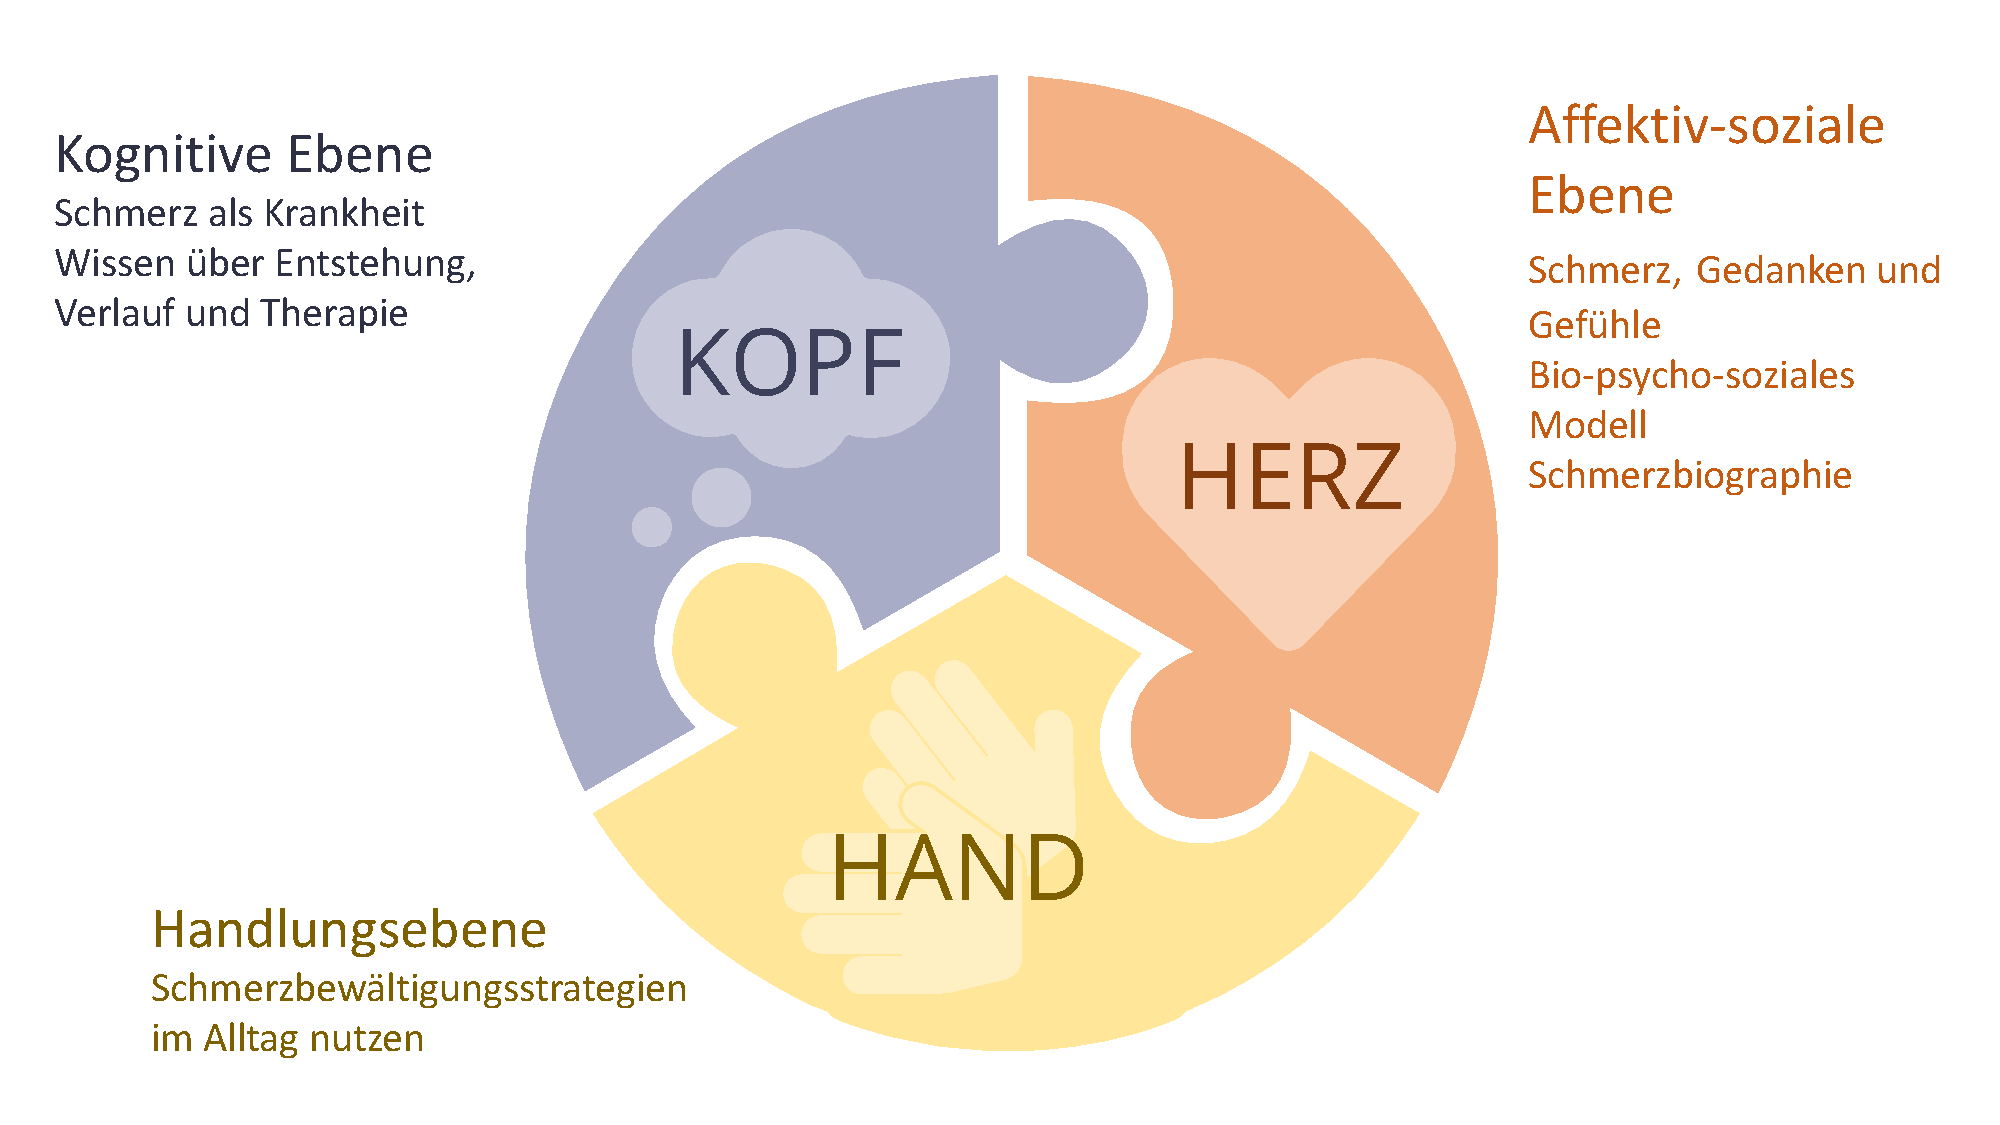
\includegraphics[width=1.1\textwidth]{Grafiken/KopfHerzHand.pdf}
  \caption{Die drei Bausteine Kopf, Herz und Hand (eigene Darstellung)}
  \label{fig:bausteine}
\end{figure}

\begin{beispiel}
  In einem der ersten Beratungsgespräche mit einer 45-jährigen Schmerzpatientin stellt sich beim Besprechen der drei Bausteine - Kopf, Herz und Hand - heraus, dass sie selbst sich als \textquote{Kopfmenschen} sieht und sich dementsprechend schon viel Fachwissen über ihre Erkrankung angeeignet hat. Obwohl sie sich auch schon in der Theorie über Schmerzbewältigungsstrategien informiert hat ist es bisher nicht gelungen, diese aktiv-handelnd im Alltag umzusetzen. Die Hinwendung zu den eigenen Gefühlen in Bezug auf das Schmerzerleben beschreibt die Patientin als sehr schwierig, da sie in einer Familie aufgewachsen ist, in der das Zeigen von Gefühlen als Schwäche ausgelegt und nicht gern gesehen wurde. Ihr ist aber bewusst, dass ihre negativen Emotionen in Bezug auf den Schmerz diesen stark beeinflussen. Es zeichnet sich also ab, dass die individuellen Lernziele in ihrem Fall den Schwerpunkt auf der affektiv-sozialen Ebene und auf der Handlungsebene haben werden. Das große fachliche Interesse sowie das hohe Maß an Bildung und Intelligenz werden als bestehende Ressourcen der Patientin identifiziert, die auch in Bezug auf die anderen Bausteine genutzt werden können. 
\end{beispiel}

\subsection{Überprüfung und Kontrolle}

Wenn die Ziele gesetzt sind kommt schnell die Frage auf, wie am Ende eigentlich überprüft werden kann, ob sie auch erreicht wurden. Stellt man den Blickwinkel eher eng und konzentriert sich auf die kognitiven Lernziele, dann kann eine konkrete Erfassung des Outputs erfolgen, bspw. mit Hilfe einer schriftlichen Prüfung. Eine Erfolgskontrolle kann jedoch nicht nur auf objektiv-messbare Art und Weise geschehen, sondern sich je nach Lernzieldimension auch subjektiv gestalten, z.B. über persönliche Rückmeldungen der Teilnehmenden. Es ist sogar zu fragen, \textquote[{\cite[98]{schlutz}}]{ob der Begriff der Kontrolle überhaupt angebracht erscheint}. Stattdessen ist bspw. eine eigene Einschätzung der Teilnehmenden über ihren Lernzuwachs denkbar, insbesondere dann, wenn statt der kognitiven die affektiv-sozialen Lernziele im Vordergrund des Angebots standen. Carl Rogers vertrat den Standpunkt, dass Prüfungen, Noten, Titel und jegliche Bewertung von Ergebnissen des Lernens abgeschafft werden müssten, da sie nichts mit signifikantem Lernen zu tun hätten: \textquote[{\cite[155]{rogersLernenFreiheit}}]{Sie messen nur den irrelevanten Typ des Lernens.}


\begin{praxis}
  Um zu überprüfen, ob die Lernziele der Einzelnen erreicht wurden, ist ein einstündiges letztes Gruppentreffen geplant, das die Evaluation des vorangegangenen Lernprozesses zum Inhalt hat \autoref{sec:ablaufplan}. Auch während der dritten Gruppensitzung ist ein Zeitfenster für eine Zwischenevaluation eingeplant. Während der Einzelgespräche, welche kontinuierlich über die gesamte Dauer des Angebots stattfinden, ist immer wieder der Blick auf die vereinbarten Lernziele zu richten und ggf. gemeinsam zu überlegen, wie diese noch besser erreicht werden können bzw. welche Hindernisse sich zu ihrem erfolgreichen Erreichen ergeben haben. Dem Grundgedanken des personzentrierten Beratungs- und Psychoedukationsangebots entspricht es, personen- und prozessorientiert zu denken; eine \textquote{Kontrolle} im Sinne einer Bewertung von außen erfolgt daher nicht. Ein Ziel gilt dann als erreicht, wenn die Lernenden sagen, dass es erreicht wurde.
\end{praxis}



\subsection{Zielsetzung vs. Vereinbarung}

Ein wichtiger Punkt, welcher jedoch nur am Rande \autocite[vgl.][99]{schlutz} oder gar nicht erwähnt wird \autocite[vgl.][]{reich-claassen} ist, dass es sich bei den Lernzielen um die Ziele der Lernenden -- nicht die der Lehrenden -- handeln soll. Im Sinne des didaktischen Prinzips der Teilnehmendenorientierung sollten die Bedürfnisse bzw. Lernbedarfe der Teilnehmenden im Mittelpunkt stehen. Lernziele stehen sozusagen im Dienst der Lernenden; sie dienen dazu, den Weg hin zu ihrem Erreichen zu erleichtern; als Planungsinstrumente helfen sie der Lehrkraft, diesen Weg didaktisch zu gestalten. Dementsprechend sollten sie von Seiten der planenden Person eher Vorschlags- als Vorschriftscharakter haben, besonders dann, wenn die Teilnahme am Angebot freiwillig erfolgt, es keinen externen Auftraggebenden gibt, keine (staatliche) Vorgabe wie bspw. ein bestimmter normierter Abschluss (Mittlere Reife; Fahrprüfung etc.) erreicht werden soll und die Lerninhalte sich im Bereich der affektiv-sozialen bzw. der Handlungs-Dimension bewegen. Es sollte für alle Arten von Angeboten gelten, dass Lernziele \textquote[{\cite[99]{schlutz}}]{[e]rst durch Erwartungsabfragen und Vereinbarungen (...) auch zu Zielen (...) der Lernenden} werden. 

\begin{praxis}
  Im großen Psychoedukations-Manual von \citeauthor{wachter} werden nicht weniger als 20 übergreifende Ziele des Programms genannt. Dieses umfangreiche Manual richtet sich eher an große schmerztherapeutische, psychosomatische und/oder Rehabilitations-Einrichtungen mit zahlreichen Mitarbeitenden und großen Patientengruppen. Für einen kleineren Rahmen im ambulanten Bereich beschränkt man sich auf ein übergeordnetes Lernziel pro Lernzieldimension:
  Nach ihrer Teilnahme am Psychoedukations- und Beratungsangebot...
  \begin{itemize}
    \item \textbf{Kognitive Dimension (Kopf)}: ...haben die Betroffenen aktuelles, evidenzbasiertes Faktenwissen über ihre jeweilige Erkrankung erhalten und verstanden; dieses Faktenwissen wird passend zu ihrem Kenntnisstand, der individuellen Bedeutsamkeit und den kognitiven Kapazitäten ausgewählt und didaktisch aufbereitet. 
    \item \textbf{Affektiv-soziale Dimension (Herz)}: ... haben die Betroffenen die Wechselwirkungen zwischen ihrer Schmerzerkrankung, ihren Emotionen und ihren Lebensumständen erkannt (bio-psycho-soziales Modell) und die Rolle der Schmerzerkrankung in ihrem Lebenszusammenhang reflektiert (Schmerzbiographie).
    \item \textbf{Handlungs-Dimension (Hand)}: ... haben die Betroffenen einen persönlichen \textquote{Werkzeugkasten} an Schmerzbewältigungsstrategien erarbeitet und sind motiviert, diese passend zur jeweiligen Anforderungssituation selbstständig einzusetzen.
  \end{itemize}

  Die jeweiligen Feinziele, welche am Ende des Psychoedukations- und Beratungsprozesses erreicht werden sollen, werden im persönlichen Gespräch zwischen Patient:innen, behandelnden Ärzt:innen und der Lernbegleiterin (Dozent:in) festgelegt. 
\end{praxis}

\begin{beispiel}
  Ein gerade 18 Jahre alt gewordener Patient leidet seit  drei Jahren an Migräneattacken, welche in den letzten Monaten an Häufigkeit zugenommen haben und zu Fehlzeiten in der Schule führen. Im heutigen Beratungsgespräch geht es darum, seine Lernziele für die drei Lernzieldimensionen festzulegen. Es stellt sich heraus, dass er sich bisher noch nicht intensiv mit der Pathophysiologie seiner Migräneerkrankung beschäftigt hat und den Entstehungsmechanismus einer Migräneattacke nicht kennt, sodass er die Wirkweise seiner Medikation falsch eingeschätzt hat und diese nicht zum korrekten Zeitpunkt und in korrekter Dosierung eingenommen hat. Ein Lernziel der kognitiven Ebene wird demnach sein, diese Wissenslücken zu schließen. Der Patient beschreibt sich selbst als eher unordentlich und chaotisch veranlagt; das Führen eines Schmerzkalenders gelang ihm bisher nicht, sodass der Überblick über die Attackenhäufigkeit und die Schmerzmitteleinnahme verloren ging. Auf der Handlungsebene wird demnach ein Ziel sein, geeignete Methoden zu finden um seinen Krankheitsverlauf so zu dokumentieren, dass daraus Implikationen für die weitere Therapieplanung erfolgen können. Der Patient erzählt, dass er sich von seinen Eltern unter Druck gesetzt fühle, da diese seinen Erfolg bei den Abiturprüfungen in Gefahr sähen, sollte er sein Chaos nicht in den Griff bekommen und die Migräne sich verschlimmern. Es besteht also auch ein Zusammenhang seiner Erkrankung mit seinen Gefühlen und dem sozialen System, in dem er lebt. Am Ende des Gesprächs notieren die Pain Nurse und der Patient gemeinsam folgende Lernziele:
\begin{itemize}
  \item \textbf{Kopf}: Erfahren, wie eine Migräneattacke entsteht und wie Schmerzmittel in diesen Prozess eingreifen und wirksam werden, um diese bei künftigen Attacken so einzusetzen, dass sie ihre optimale Wirkung entfalten können und möglichst minimale Nebenwirkungen haben.
  \item \textbf{Herz}: Erkennen, wie sich bestimmte Emotionen und Stress auf Häufigkeit und Schwere von Migräneattacken auswirken um zukünftig rechtzeitig Gegenmaßnahmen ergreifen zu können; reflektieren, welche Rolle soziale Beziehungen, insbesondere innerfamiliäre, in Bezug auf die Erkrankung spielen und herausfinden, wie diese günstig beeinflusst werden können.
  \item \textbf{Hand}: eine geeignete Methode finden, um einen Schmerzkalender regelmäßig zu führen und wichtige Daten über die Erkrankung zu sammeln; Entspannungsmethoden ausprobieren und herausfinden, wie sie in den Alltag integriert werden können.
\end{itemize} 

\end{beispiel}

Gegebenenfalls können die individuellen Lernziele auch mit einem \textquote{Ich will...} beginnen; in jedem Fall ist es wichtig, dass Patient:innen diese Ziele als gemeinsam erarbeitet, aber letztlich von ihnen selbst für sich selbst festgelegt empfinden.


\section{Was: Lerninhalte}\label{sec:was}

Da in fast allen Fachbereichen die Menge an verfügbarem Wissen unüberschaubar groß geworden ist und
stetig weiter wächst, ist eine didaktische Reduktion unabdingbar. Diese kann anhand der bekannten
Kriterien erfolgen, z.B. indem man sich auf das Grundlegende, Wesentliche einer Sache konzentriert
oder, als Gegenentwurf, das Besondere, Exemplarische hervorhebt und von diesem ausgehend auf
allgemeine Prinzipien hinweist \autocite[vgl.][23f.]{kos}. Die Lerninhalte müssen in enger
Abstimmung zu den Lernzielen ausgewählt werden. Die Frage, die sich Angebotsplanende stellen müssen,
lautet also: \textquote{Welcher Inhalt ist wirklich relevant, damit die Teilnehmenden ihre Lernziele
erreichen können?}. Hierbei ist insbesondere zu bedenken, wie die digitale Wissensgesellschaft aufgebaut ist: Welches Faktenwissen muss tatsächlich noch auswendig beherrscht werden, und wann ist es zielführender, hilfreiche Strategien, z.B. zur Informationsbeschaffung und Recherche, zu erlernen? Diese Überlegungen ziehen maßgebliche Konsequenzen für die didaktische Gestaltung des Angebots nach sich, z.B. in Bezug auf den zeitlichen Umfangs des Angebots, auf die Auswahl der passenden Methoden, Medien u.v.m. und sollten daher ausreichend Beachtung finden.

Des weiteren ist zu bedenken, dass je nach Kontext, in dem ein Angebot entwickelt wird, Inhalte in das Profil der Erwachsenenbildungseinrichtung passen oder sich an vorgegebenen Standards (bspw. der IHK) ausrichten müssen \autocite[vgl.][1008]{reich-claassen}.

\begin{praxis}
Die Lerninhalte müssen passend zu den Lernzielen ausgewählt werden; zur Vorbereitung des Angebots können für jede Lernzieldimension bereits bestimmte Themen festgelegt werden:
\begin{itemize}
  \item \textbf{Kognitive Dimension (Kopf)}: Die Patient:innen benötigen aktuelles, evidenzbasiertes Wissen über ihre jeweilige Erkrankung. Die kleine Anzahl an Teilnehmenden (3-5 Personen) ermöglicht es, einzeln zu besprechen, was jede:r bereits über die eigene Krankheit weiß - in manchen Fällen kann dies ein respektables Expert:innenwissen sein, wenn sich Betroffene schon ausführlich selbst informiert haben. In anderen Fällen fehlt es sogar am basalen Verständnis über Entstehungszusammenhänge der eigenen Erkrankung, über Wirkweise von Medikamenten und Therapien etc. Es gilt, gemeinsam herauszufinden, welches Faktenwissen benötigt wird, um zu einem besseren Verständnis der Schmerzerkrankung zu gelangen, und auf welchem Niveau Betroffene dieses Wissen verarbeiten können. Aufgabe der Lernbegleiterin ist es, in Abstimmung mit behandelnden Ärzt:innen, dieses Wissen für die Betroffenen didaktisch so aufzubereiten und zur Verfügung zu stellen, dass es optimal aufgenommen werden kann. Während der Gruppensitzungen kommen fünf Themenbereiche zur Sprache bzw. werden den Teilnehmenden als Vorschläge angeboten:
  \begin{itemize}
    \item Thema 1: Bewegung, Sport, Körperwahrnehmung
    \item Thema 2: Entspannung, Stressbewältigung, Schlaf 
    \item Thema 3: Sozialleben und Kommunikation mit/über/trotz Schmerzen
    \item Thema 4: Ernährung und Genuss 
    \item Thema 5: Lebensfreude, Interessen und Hobbys pflegen mit/trotz Schmerzen
  \end{itemize}
  
  Die Themenvorschläge sind angelehnt an die Inhalte des Psychoedukations-Manuals von \citeauthor{wachter}. 

  \item \textbf{Affektiv-soziale Dimension (Herz)}: Im Rahmen des Psychoedukations- und Beratungsangebots wird keine Psychotherapie durchgeführt; dies wird den Teilnehmenden bereits vor Beginn ihrer Teilnahme mitgeteilt. Dennoch ist es möglich, in den Beratungsgesprächen über Gedanken und Gefühle in Bezug auf die Schmerzerkrankung zu sprechen und gemeinsam zu rekonstruieren, welchen Beginn und Verlauf die Erkrankung nahm/nimmt, welchen Raum sie im Leben einnimmt, welchen Einfluss sie auf die Gestaltung sozialer Beziehungen im Privat- und Berufsleben hat etc. Verlaufsbeobachtungsbögen (z.B. als Teil des Deutschen Schmerzfragebogens; s. Anhang) oder Aktivitätstagebücher, in denen die betroffene Person tägliche Aktivitäten, die eigene Stimmung, das Vertrauen in die Wirksamkeit der Behandlung etc. einträgt, können einen Prozess der Selbstreflexion anstoßen. \footnote{Ein wünschenswerter Effekt könnte auch sein, dass Betroffene, die große Ängste und Vorbehalte gegenüber der Psychotherapie hegen, sich einer vertrauten Fachperson, die ausdrücklich kein:e Therapeut:in ist, leichter öffnen können, dahingehend positive Erfahrungen machen und über diesen \textquote{Umweg} doch noch den Mut fassen, eine (Schmerz-)Psychotherapie zu beginnen.}
  \item \textbf{Handlungsdimension (Hand)}: Um den persönlichen Werkzeugkasten zur Schmerzbewältigung zu füllen kann zur Vorbereitung des Angebots auf bereits vorliegende Literatur zurückgegriffen werden, z.B. auf das Psychoedukations-Manual von \textcite{wachter} oder die umfangreiche Sammlung von Techniken zur psychologischen Schmerzbewältigung von \citeauthor{richter}, die sowohl zum Einüben in der Gruppe als auch zum selbständigen Erlernen geeignet sind. Die Auswahl reicht von Entspannungs- und Imaginationsübungen über Methoden, die dabei helfen, eine Veränderung des eigenen Denkens, Bewertens und Erlebens anzustoßen, Ideen zum achtsameren Umgang mit sich und dem eigenen Körper bis hin zum Einsatz von technisch unterstütztem Bio- und Neurofeedback. Dabei ist immer zu bedenken, dass nicht die konkrete Aktivität oder Strategie entscheidend ist, sondern dass sie passend zur Person und deren Bedürfnissen ausgewählt wird \autocite[vgl.][336]{HeftSchmerz5}.
\end{itemize}
\end{praxis}

\begin{figure}
  \centering
  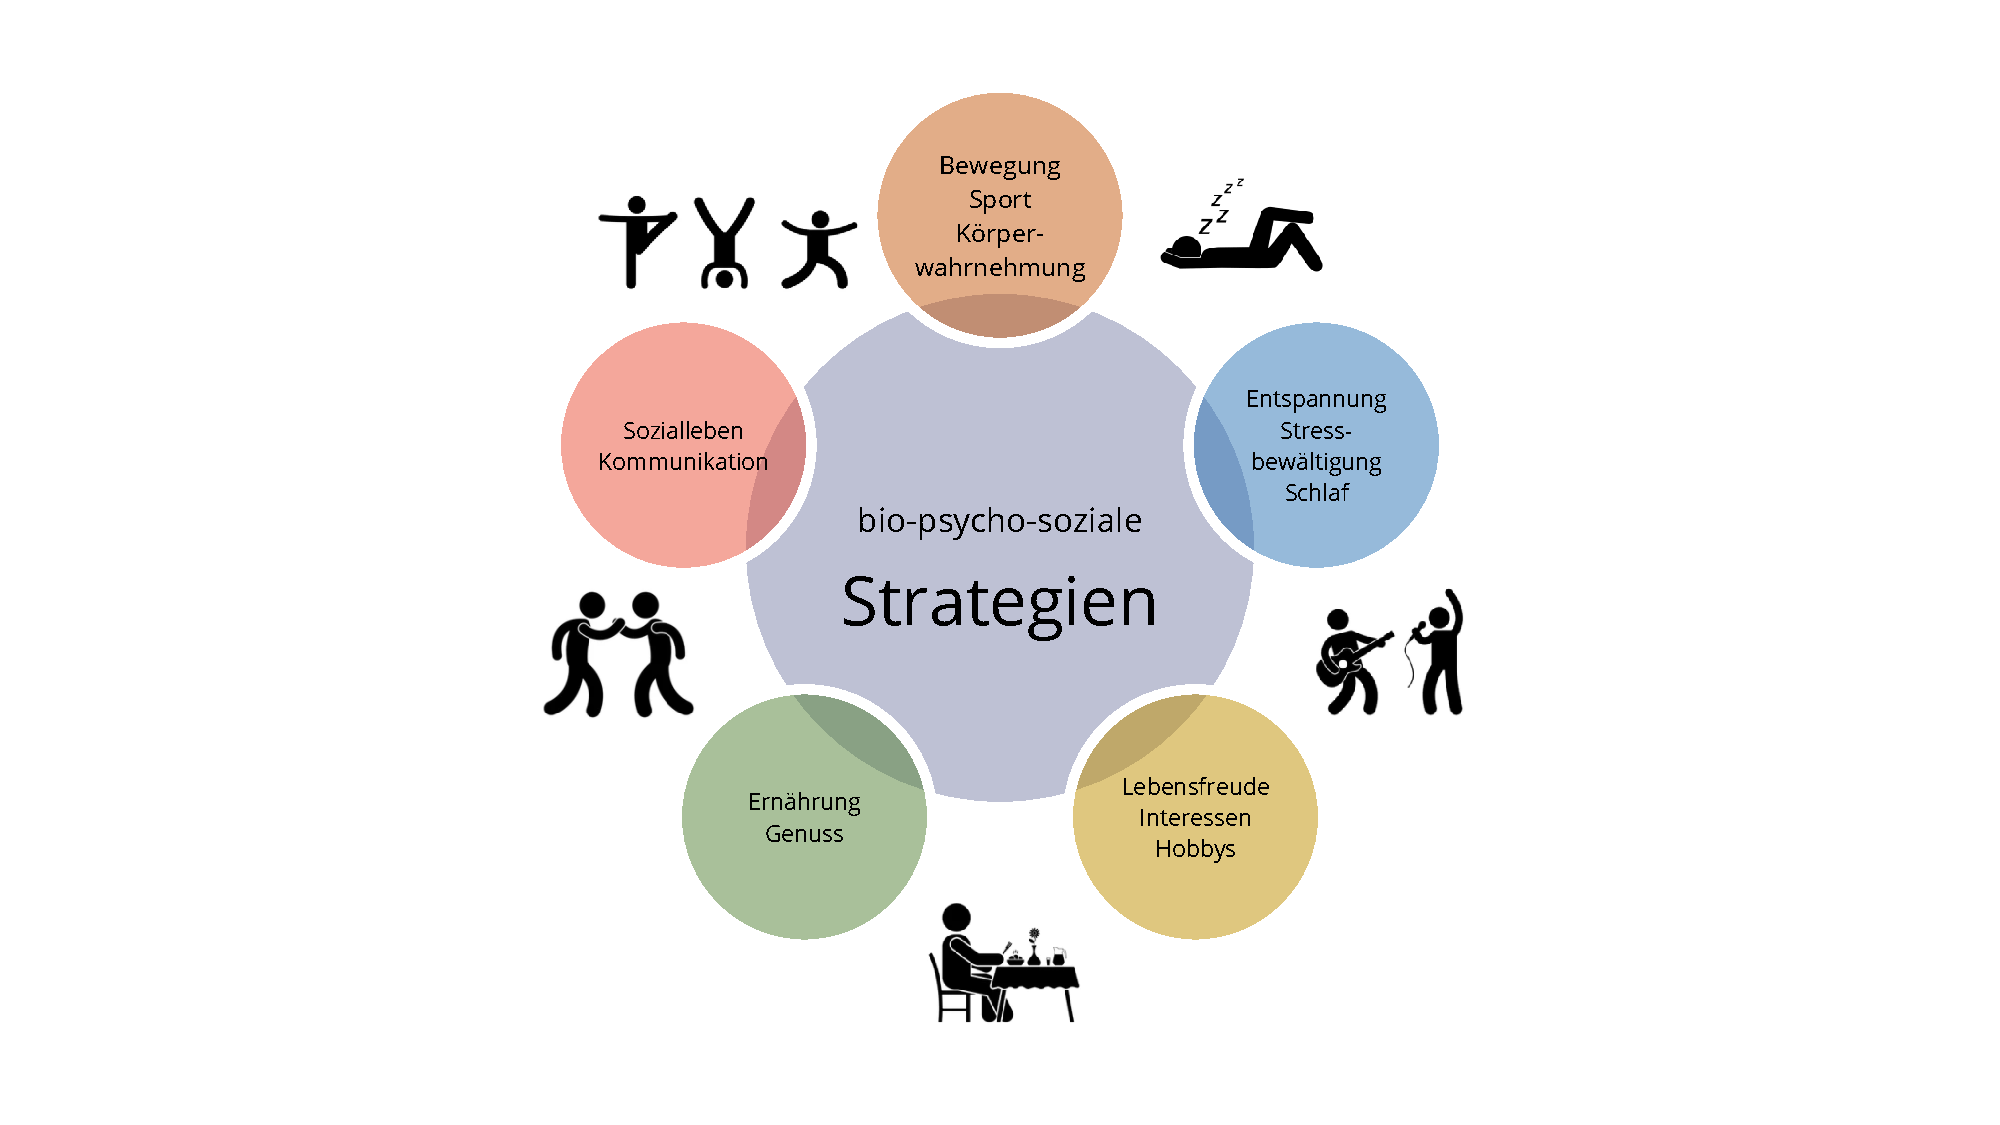
\includegraphics[width=0.7\textwidth]{Grafiken/Strategien.pdf}
  \caption{Bio-psycho-soziale Strategien der Schmerzbewältigung (eigene Darstellung)}
  \label{fig:biopsychosozial}
\end{figure}

\section{Wie: Organisationsform und Methoden}

Während der Angebotsplanungsphase muss festgelegt werden, welche Organisationsform eine Veranstaltung haben soll und in welchem zeitlichen Rahmen sie ablaufen wird. Die denkbare Auswahl aus möglichen Formen ist riesengroß und kann kreativ auf die jeweiligen Lernbedürfnisse der Zielgruppe zugeschnitten werden. Anhaltspunkte für die zeitlichen Präferenzen der Zielgruppe gibt die Bedarfsanalyse. Darüber hinaus hängt die gewählte Form auch von der didaktischen Konzeption des Angebots ab. Ob als Organisationsform ein Vortrag, ein Wochenendseminar oder ein Jahreskurs gewählt wird, muss ebenso wie die Auswahl der einzelnen Methoden innerhalb des Angebots in Einklang mit den didaktischen Prinzipien der Erwachsenenbildung (Erfahrungs-, Teilnehmenden- und Handlungsorientierung) stehen und das Erreichen der Lernziele optimal unterstützen \autocite[vgl.][1009]{reich-claassen}. Methoden sind dabei niemals als Selbstzweck zu verstehen, sondern \textquote[{\cite[102]{schlutz}}]{eröffnen vor allem den Lernenden Ansätze zur Aneignung, auch zum Arbeitskontakt mit dem Gegenstand und den Mitlernenden}. Die verschiedenen Sozial- und Aktionsformen (darunter z.B. Präsentationsformen wie Vortrag und Demonstration, Interaktionen wie Lehrgespräch und Diskussion, Aneignung- und Erkundungsformen wie Untersuchen und Problemlösen oder besondere Verfahren wie Brainstorming und Rollenspiel) müssen der Lernprozessphase angemessen und sinnvoll begründet eingesetzt werden \autocite[vgl.][101]{schlutz}.

\begin{praxis}
  Die Organisationsform des Angebots ist eine Mischung aus Gesprächsformaten (Einzel- und Gruppengespräche) sowie Selbstlernphasen, die auch zum Einüben und Ausprobieren der neuen Fähigkeiten im Alltag dienen. Als zeitlicher Rahmen wird ein halbes Jahr festgelegt; die Gespräche folgen einem bestimmten logischen Rhythmus (\autoref{sec:ablaufplan}). Die Gruppensitzungen von 120 Minuten Dauer sind als moderierte Lern- und Gesprächseinheiten konzipiert:  Nach einer Begrüßung folgt eine Vorstellungsrunde bzw. ab der zweiten Sitzung eine Runde zum Erfahrungsaustausch: Wie konnten die Teilnehmenden in der vergangenen Woche das neu Erlernte im Alltag einsetzen? Welche Erfolge können verzeichnet werden und welche Hindernisse sind zu benennen? Es folgt ein kurzer informativer Input (ein Lern-Angebot - kein Unterrichtsstoff!) durch die Lernbegleiterin oder zum Thema der heutigen Sitzung, z.B. in Form eines Kurzvortrags begleitet durch ein Videobeispiel, eine schriftliche Selbstreflexion der Teilnehmenden, ein Schaubild, eine praktische Übung, die direkt gemeinsam durchgeführt werden kann oder Ähnliches. Die Vermittlung von Wissen wird auf diese Weise immer direkt mit einer handlungs- oder erfahrungsorientierten Methode kombiniert. Es folgt eine gemeinsame Auswertung und Besprechung der Ergebnisse in der Runde; die Patient:innen werden hier zum freien Ausdruck ihrer Gedanken und Gefühle in Bezug auf das Lernangebot ermutigt. Diese werden von der Lernbegleiterin (und den anderen Teilnehmenden!) wertschätzend-empathisch aufgenommen und fließen direkt in das Abschlussgespräch der Sitzung ein: Welche Ideen kommen den Patient:innen, wie das Lernangebot in den eigenen Alltag übernommen werden kann? Hier ist von besonderer Bedeutung, dass es keine vorgegebene Hausaufgabe für alle geben kann; jede und jeder ist vollkommen frei darin, sich ein selbstgesetztes Ziel als Aufgabe mitzunehmen. Im letzten Teil der Gruppensitzung geht es um die Gestaltung der nächsten Sitzung in zwei Wochen: Welche Wünsche und Anregungen gibt es aus der Gruppe? In Abstimmung mit der Lernbegleiterin wird gemeinsam festgelegt, welches Thema auf welche Weise beim nächsten Treffen im Fokus steht.
\end{praxis}

\section{Womit und wo: Medien und Lernorte}

Lernmedien können in einem engeren oder weiteren Sinne definiert werden: Eng gefasst als \textquote[{\cite[26]{kos}}]{alle unterstützenden (multi-)medial aufbereiteten Unterlagen, die auf Papier oder in informations- und kommunikationstechnologischen Geräten zur Verfügung stehen}. Lernmedien wären demnach zum Beispiel das klassische Lehrbuch, Kursunterlagen in Form eines Handouts, aber auch Lehrvideos oder eine ganze digitale Lernplattform oder Smartphone-App. In einer weiteren Auslegung, als \textquote[{\cite[102]{schlutz}}]{Formen oder Mittel der Begegnung mit Wirklichkeit} sind Medien dagegen nicht nur Unterstützungsmittel für Lehr-Lern-Prozesse, sondern können auch selbst \textquote[{\cite[102]{schlutz}}]{Träger des Geschehens} werden. So kann auch der Lernort als Medium begriffen werden, sofern er direkt mit den Lerninhalten verknüpft ist, bspw. bei einer Exkursion, oder besondere Lern- und Sozialformen ermöglicht, bspw. Gruppenarbeit in Präsenz oder interaktives Online-Learning \autocite[vgl.][102]{schlutz}. \citeauthor{reich-claassen} weisen darauf hin, dass auch bei der Auswahl von Medien und Lernorten die drei besonders wichtigen didaktischen Prinzipien der Erwachsenenbildung die Richtung vorgeben sollen: Erfahrungs-, Teilnehmenden- und Handlungsorientierung betonen \textquote[{\cite[1009]{reich-claassen}}]{die Verantwortlichkeit des lernenden Subjekts}, dessen Weiterlernen immer auf den persönlichen Vorerfahrungen aufbaut. Sie empfehlen daher, auch Medien und Lernorte passend zu den Lernbedürfnissen der Teilnehmenden auszuwählen, direkte Bezüge zur Lebenswelt der Lernenden herzustellen und erfahrungsorientierte Medien einzusetzen, z.B. die \textquote[{\cite[1010]{reich-claassen}}]{aktive Videoarbeit}.

\begin{praxis}
  Lernort wird in erster Linie die Arztpraxis sein. Deren Räume sind den Teilnehmenden in der Regel schon jahrelang bekannt und vertraut. Das Wartezimmer kann auf interessante Weise zu einem Ort für die Gruppengespräche umfunktioniert werden: Vom Raum, in dem man passiv darauf wartet, abgeholt und behandelt zu werden, hin zu einem Raum, der mit Eigenaktivität und neuen Impulsen gefüllt wird. Während sich die Wartenden in der Regel sitzend anschweigen, können die Teilnehmenden nun andere Betroffene kennen lernen und in einen Austausch kommen. Die Arztpraxis als halb-öffentlicher Ort bietet die Möglichkeit, in einer geschützten, ruhigen Umgebung zu lernen und dabei nicht die Atmosphäre eines anonymen Klassenzimmers, bspw. an einer Volkshochschule (oder, wie bei Selbsthilfegruppen üblich, in Schulungsräumen des Gesundheitsamts), zu spüren. Selbstverständlich muss dafür gewährleistet sein, dass die Gruppentreffen außerhalb der Öffnungszeiten der Praxis, am besten abends, stattfinden können. Für die Einzelgespräche steht ein Beratungszimmer zur Verfügung, welches auch Informationsmaterialien wie Flyer, Broschüren und Schulungsunterlagen bereit hält.\footnote{Diese werden in hochwertiger Qualität von medizinischen Fachgesellschaften, z.B. der Deutschen Migräne- und Kopfschmerzgesellschaft, kostenlos angeboten. Auch Material von Pharmaunternehmen kann äußerst aufwendig gestaltet und hilfreich sein, z.B. bei Neueinstellung eines Betroffenen auf ein bestimmtes Medikament. In jedem Fall müssen diese externen Unterlagen zuerst auf ihre inhaltliche und didaktische Qualität hin überprüft werden, bevor sie an Patient:innen ausgegeben werden. Auch eine einseitige Einflussnahme aus der Pharmaindustrie muss immer kritisch mitgedacht werden.} Als Lernmedien sind des weiteren kostenlose oder auf Rezept verordnungsfähige Smartphone-Apps denkbar (z.B. digitale Schmerztagebücher, Programme zur Erfassung von Triggerfaktoren bei Migräne und Kopfschmerzen, Apps mit Anleitungen für Entspannungs- und Meditationsübungen), Patientenratgeberliteratur in Form von Büchern/Arbeitsblättern oder Webseiten bzw. Online-Foren (z.B. \textit{Headbook.me}, ein professionell betreutes Angebot der Schmerzklinik Kiel). Bei all der großen, bunten Auswahl an möglichen Lernmedien darf nicht vergessen werden, dass das Medium niemals zum Selbstzweck werden darf, sondern es stets um die Frage geht: Welches Medium ist am besten geeignet, um \textit{dieser} betroffenen Person bei der Erreichung \textit{ihrer} individuellen Lernziele zu helfen? 
\end{praxis}

\begin{figure}
  \centering
  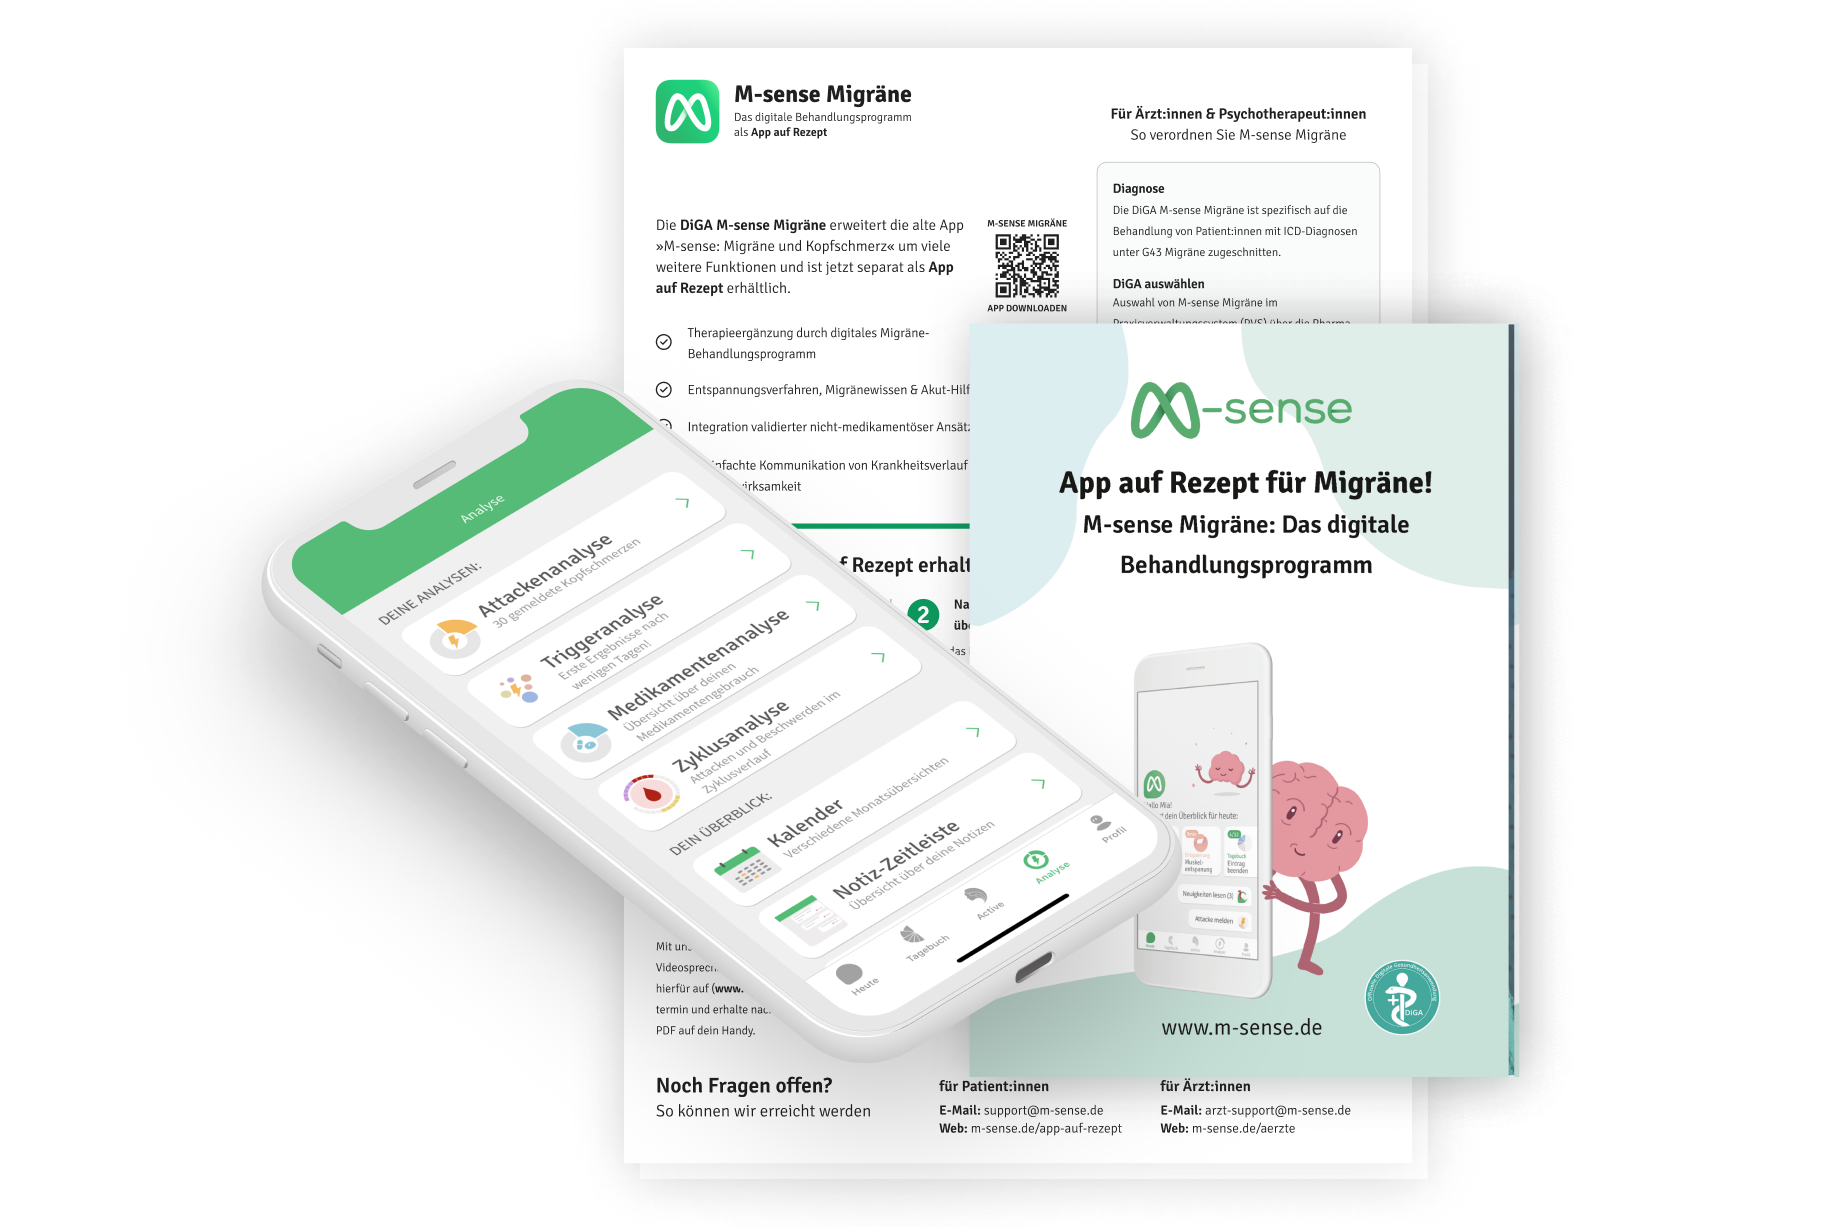
\includegraphics[width=0.5\textwidth]{Grafiken/Infopaket_M-sense_Migraene-2.png}
  \caption{Beispiel für eine sog. Digitale Gesundheitsanwendung: m-sense bei Migräne (Quelle: \url{m-sense.de})}
  \label{fig:msense}
\end{figure}

\section{Wer: Dozent:in}\label{sec:wer}
\citeauthor{reich-claassen} fügen den sechs Strukturelementen noch ein siebtes hinzu, nämlich die Frage nach dem \textquote[{\cite[1010]{reich-claassen}}]{Wer?} Sie merken an, dass \textquote{die \textquote{Passung} zwischen Dozent, Thema und v.a. der anvisierten Zielgruppe ein nicht zu unterschätzender Planungsaspekt} sei \autocite[1010]{reich-claassen}. Die Bedeutung der Lehrperson wird von allen Zielgruppen durchweg als sehr hoch eingeschätzt und ist daher ein wichtiger Faktor für das Gelingen eines Bildungsangebots. In der Phase der Angebotsplanung ist es daher lohnend, sich darüber Gedanken zu machen, welche Qualifikationen, sowohl pädagogisch-didaktischer Art als auch im jeweiligen Fachbereich, Dozent:innen haben sollten. Lehrende sollten die Bedürfnisse ihrer anvisierten Zielgruppe gut kennen und sich bewusst machen, dass sie ggf. selbst einem anderen Milieu entstammen als die Teilnehmenden \autocite[vgl.][1011]{reich-claassen}. Nicht zuletzt muss berücksichtigt werden, dass Lehrende nicht als fachliche oder didaktische Maschinen agieren -- so wichtig gute Fähigkeiten in diesen Bereichen auch sind. Menschliche Qualitäten wie Kommunikations- und Sozialkompetenz, Einfühlungsvermögen, aufrichtiges Interesse an den Lernbedürfnissen der Teilnehmenden, eine respektvolle Haltung ihnen gegenüber sowie ein stabiles eigenes Selbstkonzept als Lehrperson dürfen nicht fehlen. Auch die Reflexion über eigene Erwartungen und Motivationen gehört zum professionellen Handeln.

\begin{praxis}
  Dozent:innen für das geplante Psychoedukations- und Beratungsangebot sollen ausgebildete Medizinische Fachangestellte sein (eine Person pro Gruppe), welche über die Zusatzbezeichnung \textit{Algesiologische Fachassistenz/Pain Nurse} der Deutschen Schmerzgesellschaft verfügen.\footnote{Das Curriculum ist einsehbar unter \url{https://www.schmerzgesellschaft.de/fileadmin/2021/pdf/DS_Currciulum_Schmerzmanagement_Pflege_20102021_Screen.pdf}, aufger. am 12.12.2021} Es handelt sich hierbei um eine Zusatzqualifikation, welche medizinisch vorgebildete Fachpersonen aus Pflegeeinrichtungen oder ambulanten Praxen erwerben können \autocite[vgl.][193]{nobisHerausforderung}. Es werden in mehrtägigen Grund- und Aufbaukursen fachliche, soziale und methodische Kompetenzen vermittelt, um Schmerzpatient:innen mit einem erhöhten Maß an Eigenverantwortung mitbetreuen zu können \autocite[vgl.][193]{nobisHerausforderung}. Neben dieser erweiterten medizinischen Kompetenz müssen Dozent:innen sehr gute pädagogische und didaktische Fähigkeiten mitbringen, um \textit{facilitators} \autocite[110]{rogersLernenFreiheit}) sein zu können. Dozent:innen müssen darüber hinaus den personzentrierten Ansatz nach Carl Rogers sowohl in der Theorie kennen als auch in Beratungsgesprächen bereits praktisch erprobt und einige Erfahrung gesammelt haben. Beratung an sich ist bereits Teil des Berufsprofils Medizinischer Fachangestellter bzw. Algesiologischer Fachassistent:innen: \textquote[{\cite{BZGABeratungEdukation}}]{Im Gesundheitswesen hat Beratung seit jeher einen relativ hohen Stellenwert und gehört zu den angestammten Aufgaben der Gesundheitsprofessionen.}

  Um sicherzustellen, dass alle medizinischen Fachfragen zuverlässig und kompetent gehandhabt werden müssen die behandelnden Ärzt:innen bereitstehen, um Patient:innen auch während der Teilnahme am Angebot zu begleiten, laufende Therapien zu überwachen etc.  Gegebenenfalls können auch weitere relevante Akteur:innen miteinbezogen werden, je nach Bedarf und Wunsch der Betroffenen (beispielsweise aus der Psycho-, Physio-, Ergotherapie, Logopädie, aus ambulanten Seelsorge- oder Pflegeteams etc.) Die Frage soll stets sein: Wer kann hilfreich sein, um den Schmerzpatient:innen auf ihrem Weg eine Stütze zu sein? Professionelle Vernetzung statt Abgrenzung soll hier im Vordergrund stehen. Schmerzpatient:innen vermissen häufig nicht nur ein ganzheitliches, sondern auch ein interprofessionelles Denken im Behandlungsteam sowie eine intensive Teamkommunikation \autocite[vgl.][338]{HeftSchmerz5}. Es ist demnach ebenso Aufgabe der \textit{facilitators}, die einzelnen Akteur:innen der Schmerzbehandlung miteinander in Kontakt zu bringen, und zwar in Abstimmung und nach Wunsch der Betroffenen.
\end{praxis}

\section{Strukturplan des Angebots}\label{strukturplan}
Dieser Strukturplan entspricht weitgehend der Vorlage von \citeauthor[91]{schlutz}.
\begin{center}
  \def\arraystretch{1.5}
  \begin{longtable}{p{0.9\textwidth}}
    \hline
    \bfseries 0. Titel des Angebots \\\hline
    Personzentriertes Psychoedukations- und Beratungsangebot für Menschen mit chronischen   Schmerzerkrankungen \\\hline
    \bfseries 1. Lebens- und Verwendungssituation (Wofür?) \newline
    Lebenshintergrund, Anforderungen der Praxis, Soll-Horizont \\\hline
    \begin{itemize}[nosep, topsep=-10pt]
    \item	Menschen mit chron. Schmerzerkrankungen unterstützen und befähigen, ihr Leben möglichst selbstbestimmt zu führen
    \item Soll-Horziont: Maximum an Lebensqualität $\rightarrow$ Lebensqualität wird individuell definiert
    \end{itemize} \\\hline
    \bfseries 2. Zielgruppe/Bedarf (Für wen?)\newline
    Merkmale, Motivation, Ist-Stand, mögliche Eigenleistungen \\\hline
    \begin{itemize}[nosep, topsep=-10pt]
    \item	Erwachsene mit chronischen Schmerzen in regelmäßiger neurologischer Behandlung 
    \item	Ist-Stand: subjektiv wahrgenommene starke Einschränkung der Lebensqualität
    \item	Motivation: eigener Wunsch, durch längerfristige Begleitung und Eigenleistung die eigenen Fähigkeiten zur Schmerzbewältigung zu steigern
    \item	Eigenleistung: Bereitschaft und Motivation zur Veränderung, freiwillige Teilnahme, Bereitschaft, sich offen und aktiv in die Gespräche einzubringen
    \end{itemize} \\\hline
    
    \bfseries 3. Lernziele/Qualifikationen (Wozu?)\newline 
      Ziele des Angebots; hauptsächliche Lernformen und -leistungen; mögliche Ergebniskontrollen \\\hline
    \begin{itemize}[nosep, topsep=-10pt]
    \item Lernzieldimension 1 (kognitive Ebene): Faktenwissen über Erkrankung erhalten und verstehen
    \item Lernzieldimension 2 (affektiv-soziale Ebene): Bio-psycho-soziales Modell der Entstehung von chron. Schmerzen verinnerlichen und eigene Schmerzbiographie reflektieren
    \item Lernzieldimension 3 (Handlungsebene): Schmerzbewältigungsstrategien erlernen und in konkreten Alltagssituationen einsetzen können
    \end{itemize} \\\hline
    \bfseries 4. Inhalte/Themen (Was?) \\\hline
    \begin{itemize}[nosep, topsep=-10pt]
    \item Faktenwissen gemäß dem individuellen Bedarf der Teilnehmenden
    \item Themenbereiche der Gruppengespräche: 
    Bewegung, Sport, Köperwahrnehmung,
    Entspannung, Stressbewältigung, Schlaf,
    Sozialleben und Kommunikation,
    Ernährung und Genuss,
    Lebensfreude, Interessen, Hobbys
    \end{itemize} \\\hline
    \bfseries 5. Organisationsform und Methoden (Wie?) \newline
    Veranstaltungsform/Zeit, Ablaufgliederung, Hauptmethoden \\\hline
    \begin{itemize}[nosep, topsep=-10pt]
    \item Veranstaltungsform: Mischung aus Einzel- und Gruppengesprächen im Wechsel
    \item Zeitlicher Rahmen: 6 Monate, währenddessen ca. 10-15 Einzelgespräche pro TN (zu je 30-60 Minuten) und 6 Gruppensitzungen (zu je 120 bzw. einmalig 60 Minuten)
    \item Hauptmethoden: personzentrierte Beratungsgespräche, Kurzvorträge, moderierte Gruppendiskussion; anwendungsorientierte Methoden durch unmittelbares Einüben von Techniken zu Schmerz- und Stressbewältigung.
    \end{itemize} \\\hline
    \bfseries 6. Lernort und Medien (Wo und womit?) \newline
    Virtuelle und besondere Lernorte, Bedarf an Hilfsmitteln/Medien \\\hline
    \begin{itemize}[nosep, topsep=-10pt]
    \item Lernort (Fach-)Arztpraxis; Wartezimmer wird umgestaltet zu Gruppen- und Übungsraum
    \item Hilfsmittel: Informations- und Schulungsmaterial in Papierform oder digital; digitale Präsentation mit Bildschirm/Beamer/Leinwand 
    \end{itemize} \\\hline
    \bfseries 7. Dozent:in (Wer?) \newline
    Notwendige Qualifikation, Haltung gegenüber der Gruppe, Vorbereitungsleistung, Zeitaufwand \\\hline
    \begin{itemize}[nosep, topsep=-\parskip]
    \item Medizinische Vorkenntnisse und entsprechende Ausbildung mit Schwerpunkt Versorgung von Menschen mit chronischen Schmerzen
    \item Pädagogisch-didaktische Fähigkeiten, um Lerneinheiten hochwertig und flexibel vorbereiten bzw. an Gruppenbedürfnisse anpassen zu können
    \item Kenntnisse der personzentrierten Gesprächspsychotherapie bzw. Beratung nach C. Rogers; empathische und wertschätzende Haltung gegenüber den TN
    \item Fachmedizinische Unterstützung durch Ärzt:in
    \item Zeitaufwand insgesamt ca. 91 Stunden, siehe \autoref{fig:zeitaufwand}.
    \end{itemize} \\\hline
  \end{longtable}
\end{center}


\section{Verlaufsplan des Angebots}\label{sec:ablaufplan}
Für das gesamte Angebot ist eine Dauer von einem halbem Jahr vorgesehen. Diese lange Zeitspanne ist sinnvoll, da es sich um Menschen mit einer chronischen Schmerzerkrankungen handelt, die schon wesentlich länger als ein halbes Jahr besteht, durchschnittlich sieben bis 20 Jahre \autocite[vgl.][]{Schmerzgesellschaft}. Sechs Monate entsprechen zwei Abrechnungsquartalen (die in einer Arztpraxis übliche Einteilung des Jahres) bzw. 24 Wochen. Es wird davon ausgegangen, dass eine Pain Nurse während dieser Zeitspanne vier Patient:innen betreuen kann, die gleichzeitig an dem Angebot teilnehmen. Diese Anzahl resultiert aus der Überlegung, dass es Phasen mit Einzelgesprächen geben soll, denen mindestens eine Stunde Zeit zur Verfügung stehen sollte. Pro Woche wären dies vier Stunden reine Gesprächszeit und somit Arbeitszeit, welche im normalen Praxisbetrieb fehlt. Zudem soll es Gruppenphasen geben, in denen sich die Teilnehmenden kennen lernen und ausreichend Raum haben sollen, um sich zu äußern, Fragen zu stellen und Erfahrungen zu teilen. Eine zu große Gruppe würde diesen Freiraum für den Einzelnen zu stark beschneiden.

\begin{figure}[h!]
\centering
\begin{tikzpicture}[
  every node/.style={
    align=center,
    minimum height=5cm,
    text=white,
    anchor=west,
    inner xsep=5pt,
  }
]
  \definecolor{blueish}{RGB}{126,131,220}
  \definecolor{blueish2}{RGB}{46,117,182}
  \definecolor{orangish}{RGB}{232,79,54}
  \definecolor{greenish}{RGB}{84,180,53}
  \node[
    fill=blueish!80!gray,
    text width=170pt,
   ] (A)
   {
    4 Teilnehmende, pro TN 14 Einzelgespräche zu 45 Minuten + 15 Minuten Vor-/Nachbereitungszeit für Dozent:in \\[15pt]
    \large\bfseries 56 Stunden
   };
   \node[
    text width=90pt,
    fill=blueish2!80!gray,
    xshift=5pt,
   ] (B) at (A.east)
   {
     5 Gruppensitzungen zu 120 Minuten + 1 Gruppensitzung zu 60 Minuten \\[15pt]
     \large\bfseries 11 Stunden
   };
   \node[
    text width=110pt,
    fill=orangish!30!blueish!80!gray,
    xshift=5pt,
   ] (C) at (B.east)
   {
    Geschätzte Vor- und Nachbereitungszeit pro Gruppensitzung: 4 Stunden \\[15pt]
    \large\bfseries 24 Stunden
   };

   \node[
     fill=greenish!80!white,
     yshift=-5pt,
     text width=170pt + 90pt + 110pt + 30pt,
     anchor=north west,
     line width=1.5pt,
     minimum height=1cm,
   ] at (A.south west)
   {
     \Large Zeitaufwand: \bfseries 91 Stunden
   };
\end{tikzpicture}
\caption{Schätzung des Zeitaufwands (eigene Darstellung)}
\label{fig:zeitaufwand}
\end{figure}

Der Verlaufsplan sieht also wie folgt aus:

\begin{figure}[h!]
  \centering
  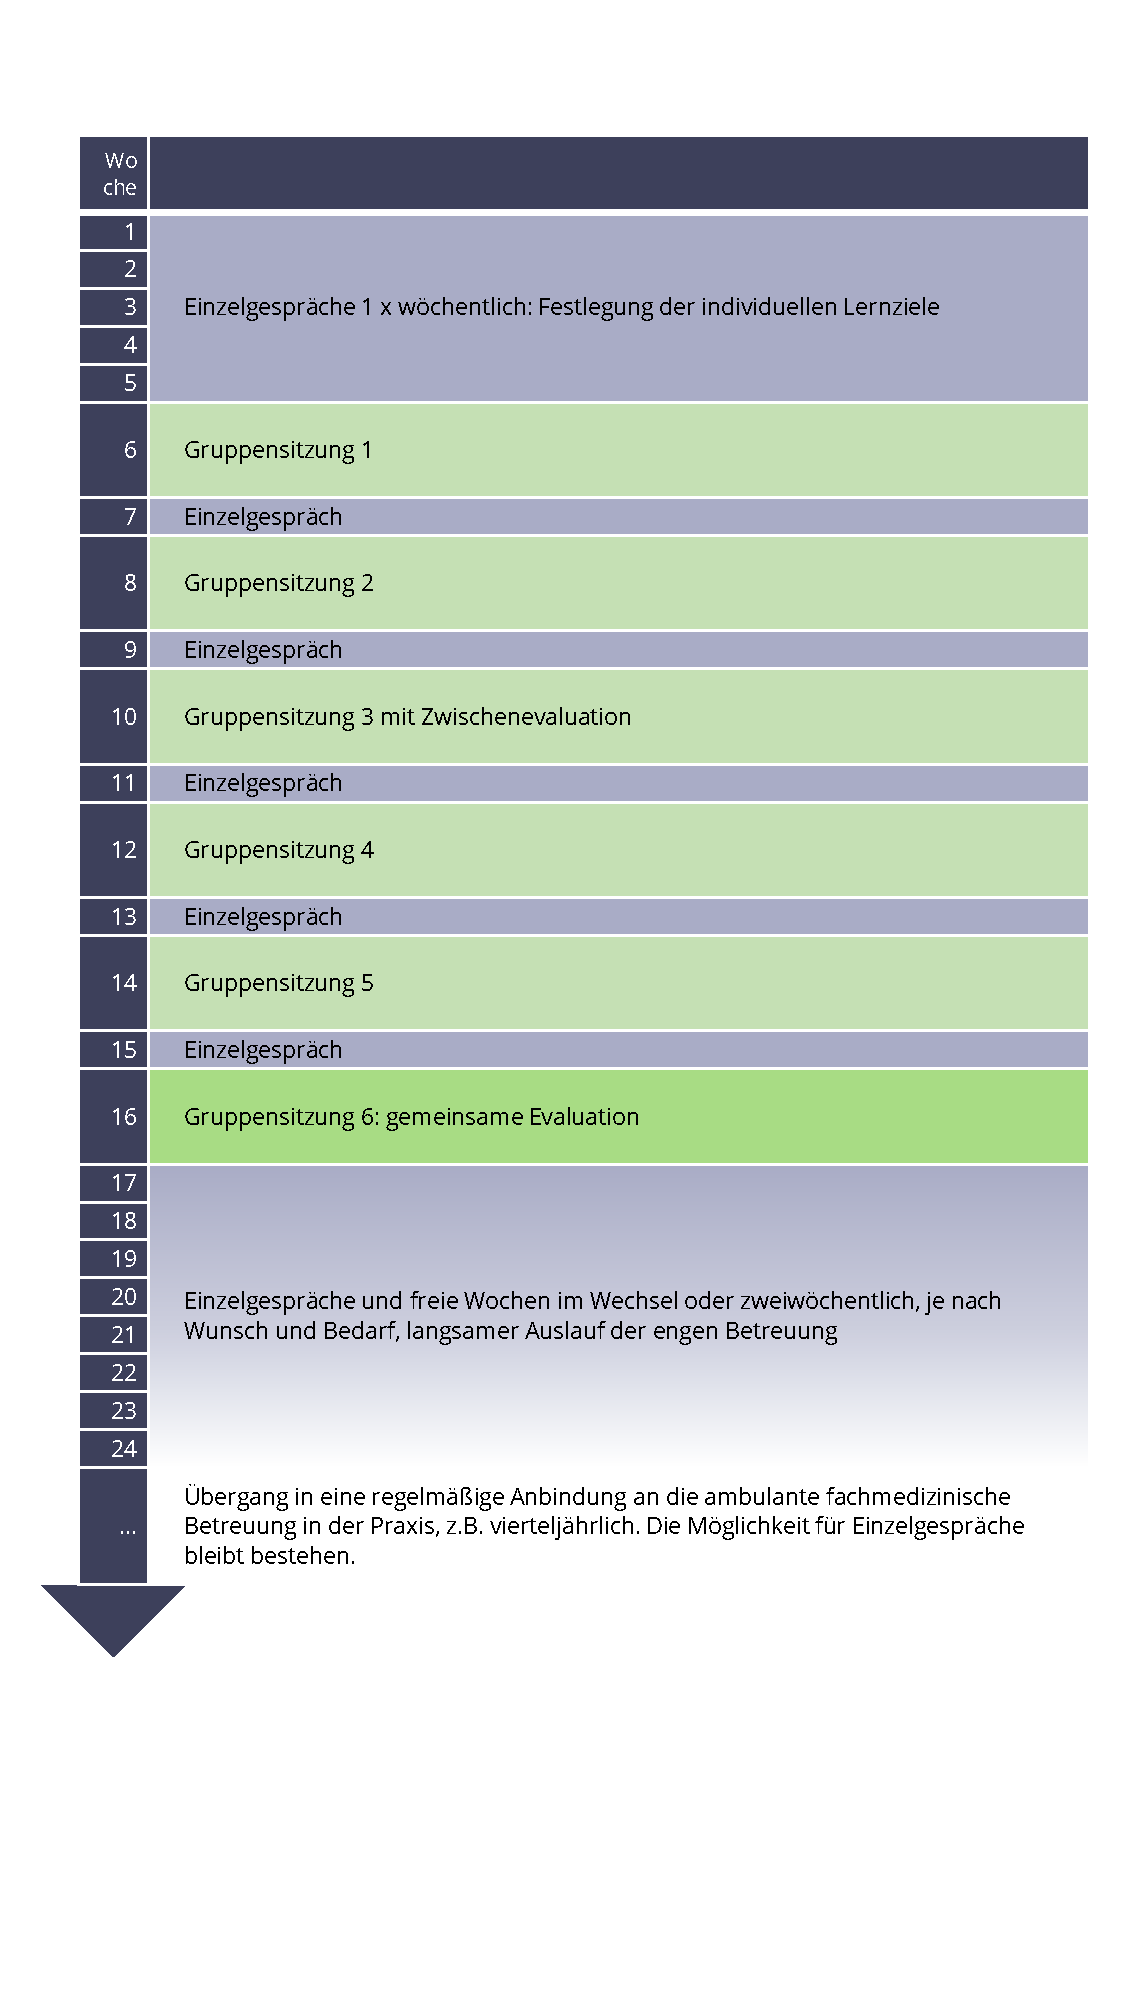
\includegraphics[height=0.9\textheight]{Grafiken/Ablaufplan.pdf}
  \caption{Verlaufsplan (eigene Darstellung)}
  \label{fig:ablaufplan}
\end{figure}

Von Woche 1 bis Woche 5 vereinbart jeder der vier Teilnehmenden pro Woche ein Gespräch mit der Pain Nurse. Nach Bedarf werden diese Gespräche auch gemeinsam mit der behandelnden Ärzt:in geführt. Diese ersten fünf Gespräche dienen zunächst dem Kennenlernen und widmen sich im Anschluss dem gemeinsamen Sondieren und Festlegen der konkreten Lernziele für die betroffene Person. Hier kommt ein Fragebogen zum Einsatz: Der Deutsche Schmerzfragebogen (DSF) wurde von der Deutschen Schmerzgesellschaft entwickelt und wissenschaftlich evaluiert (s. Anhang). Er dient dazu, sich einen Überblick über die wichtigsten Eckdaten zur vorliegenden Schmerzerkrankung und ihren Begleiterscheinungen zu machen. Die gemeinsame Besprechung des Fragebogens liefert erste Hinweise für das Erkennen  der individuellen Ressourcen und derjenigen Bereiche, die noch als defizitär erlebt werden. Aus diesen werden dann die eigenen Lernziele abgeleitet. 

Zwischen Woche 6 und Woche 16 findet eine zehnwöchige Phase statt, in der Gruppensitzungen und Einzelgespräche im wöchentlichen Wechsel stattfinden. In fünf Gruppensitzungen von je 120 Minuten Dauer kommen fünf Themenbereiche zur Sprache bzw. werden den Teilnehmenden als Vorschläge angeboten (\autoref{sec:was}). Die Reihenfolge der Themen ist variabel; um personzentriert vorzugehen bietet es sich an, auf die Stimmen aus der Gruppe zu hören, welche Thematik als nächstes von Interesse ist und schon vorab die Frage zu stellen, welche konkreten Wünsche in Bezug auf den Lerninhalt (Was?) und Methodik (Wie?) von den Teilnehmenden gewünscht wird.

\begin{praxis}Ein Beispiel soll diesen wichtigen Punkt verdeutlichen: Angenommen, die Gruppe äußert den Wunsch, das Thema Entspannung anzugehen. Einige berichten über negative Erfahrungen aus Aufenthalten in Kliniken, bei denen lediglich die Technik \textquote{Progressive Muskelentspannung nach Jacobson} gelehrt wurde, die aber ohne Erfolg geblieben ist. Die Gruppe interessiert sich stärker für Verfahren, die in Richtung Achtsamkeit und Meditation gehen und möchte diese auch gern praktisch ausprobieren. Personzentriertes pädagogisches Handeln erfordert hier Flexibilität im Sinne einer situativen Unterrichtsplanung, denn \textquote[{\cite[48]{arnold}}]{Je offener und situativer die Prozessgestaltung ist, desto größer ist die Chance auf Angepasstheit auf die Situationen der Lernenden.} 
  
  Gemeinsam wird also überlegt, wie diesem Lernbedürfnis der Gruppe nachgekommen werden kann. Weiß die Dozentin als medizinisch vorgebildete Pädagogin selbst genug über das Thema, um eine Lerneinheit vorbereiten zu können, welche dann ggf. erst beim übernächsten Treffen stattfinden wird? Kann vielleicht ein/e Expert:in von außen in die Gruppe eingeladen werden, z.B. ein/e Meditationslehrer:in? Gibt es verfügbare Hilfsmittel, z.B. Videoanleitungen oder Apps, die einen Einblick in die Thematik geben können? Entscheidend ist dabei die Haltung der Pädagogin gegenüber der Gruppe: Sie begreift sich als diejenige, deren professioneller Beitrag darin besteht, die Gruppe zu begleiten und Lernen zu \textit{ermöglichen} - ohne vorgefertigte Konzepte gegen die Bedürfnisse der Einzelnen durchzusetzen und ohne den Selbstanspruch, bereits zu Beginn des Angebots alles kennen und wissen zu müssen, was die Teilnehmenden brauchen - denn dies wird sich erst in der direkten Interaktion und im Lernprozess herausstellen.
\end{praxis}

Übergeordnetes Ziel während der Gruppenphase ist, den Teilnehmenden den vertrauensvollen Austausch unter Gleichen zu ermöglichen, selbstverständlich unter der gewissenhaften gegenseitigen Vereinbarung, Vertraulichkeit zu wahren. In einem entspannten und wertschätzenden Lernklima werden Strategien erlernt, welche dann in der folgenden Woche, die wieder einem Einzelgespräch gewidmet ist, im Alltag ausprobiert werden können. Die Erfahrungen aus dieser Woche können dann wiederum zum Einstieg in die nächste Gruppenrunde mitgebracht werden.

Dozent:innen kommt hierbei die Aufgabe zu, die Themenblöcke didaktisch aufzubereiten, flexibel an die Bedürfnisse der Lerngruppe anzupassen und darauf zu achten, dass weder Unter- noch Überforderung der Lernenden entsteht. Sie leiten und moderieren die Gruppengespräche, folgen dabei jedoch keinem strikten, womöglich sogar minutengenau getakteten \textquote{Stundenablaufplan}, sondern geben der Dynamik innerhalb der Gruppe Raum. 

Das sechste und letzte Gruppentreffen in Woche 16 dauert nur ca. 60 Minuten und dient der Rückschau und gemeinsamen Evaluation: Welche Strategien haben sich als hilfreich erwiesen? Welche Inhalte sind besonders im Gedächtnis geblieben? Konnte bereits eine Veränderung in Bezug auf das Schmerzerleben wahrgenommen werden? Was brauche ich in der letzten Phase des Angebots?

Diese letzte Phase dient als Zeitraum des behutsamen Abbaus der engen Betreuung durch das Team aus Ärzt:in, Dozent:in und des unterstützenden sozialen Raums der Gruppe. Die kommenden acht Wochen stehen den Teilnehmenden zur Verfügung, um weitere Einzelgespräche zu vereinbaren, am besten im zweiwöchigen, später vielleicht auch im dreiwöchigen Rhythmus. Grundgedanke dieser Ablösungsphase ist, die Teilnehmenden nicht von einem Tag auf den anderen wieder allein sich selbst, der Erkrankung und dem Alltag zu überlassen (wie es häufig nach Reha- und Klinikaufenthalten der Fall ist), sondern einen allmählichen Übergang zu schaffen, der wiederum nach den Bedürfnissen des Einzelnen gestaltet werden kann. 

\addchap{Zusammenfassung und Ausblick}

Das zukünftige Angebot hat nun eine ausführliche Planungsphase durchlaufen. Es liegen ein didaktisches Konzept, ein Strukturplan sowie ein Verlaufsplan vor, welche im nächsten Schritt die Basis für die Umsetzung des Angebots bilden. In der Umsetzungsphase rücken neue Aspekte in Bezug auf das Angebot in den Fokus, zum Beispiel die Frage nach einer sinnvollen \textbf{Kommunikations- und Marketingstrategie}, um das Angebot bei der anvisierten Zielgruppe bekannt zu machen, sowie nach der \textbf{Finanzierung}. Im konkreten Fall müssten hier Überlegungen angestellt werden, welcher finanzielle Aufwand entstehen würde (Entlohnung der Dozent:innen, Materialkosten) und ob dieser ausschließlich durch Teilnahmegebühren gedeckt werden muss oder ob es Möglichkeiten gibt, die Krankenkassen an der Finanzierung zu beteiligen, z.B. indem das Angebot als Gesundheitskurs anerkannt wird. 

Darüber hinaus ist es notwendig, dass die Beteiligten im Inneren Umfeld, in dem das Angebot stattfinden soll (bspw. einer Haus- oder Facharztpraxis), überlegen, wie das Angebot, das ja aus Einzel- und Gruppengesprächen zusammen gesetzt ist, zeitlich und organisatorisch in die bestehenden \textbf{betrieblichen Abläufe} integriert werden kann. 

Um eine kontinuierliche Verbesserung des Angebots zu ermöglichen wurden in den Verlaufsplan bereits Zeiträume für eine \textbf{Zwischen- und eine Abschlussevaluation} in der Gruppe eingeplant. In der Umsetzungsphase müssten noch konkretere Überlegungen angestellt werden, auf welche Weise die Lernergebnisse erfasst und dokumentiert werden können, bspw. indem die Teilnehmenden ergänzend zum Gespräch in der Gruppe einen kurzen Fragebogen schriftlich ausfüllen. Sehr gut denkbar wäre auch eine sogenannte \textbf{\textquote{Produktklinik}}, bei der es darum geht, \textquote[{\cite[1013]{reich-claassen}}]{Veranstaltungskonzepte (...) von der anvisierten Zielgruppe testen zu lassen bzw. die anvisierten Zielgruppen in den Entwicklungs- und Konzeptionsprozess einzubeziehen.} Patient:innen könnten so direkt an der Angebotsentwicklung beteiligt werden und eigene Wünsche und Bedürfnisse einbringen. Das didaktische Prinzip der Teilnehmendenorientierung würde auf diese Weise noch weiter hervorgehoben.

Nach erfolgreichem Abschluss der Produktklinik und vorgenommenen Anpassungen und Verbesserungen kann das Angebot regulär beginnen und es wäre bei entsprechender Nachfrage auch ein \textbf{Ausbau der Kapazität} denkbar. Es könnten mehrere Teilnehmenden-Gruppen parallel zeitversetzt laufen, sodass ein größerer Kreis an Patient:innen profitieren kann. Dafür müssten allerdings auch die entsprechenden zeitlichen und personellen Ressourcen zur Verfügung stehen. Auch eine \textbf{Umwandlung in ein digitales Lern-Angebot}, bei dem die Teilnehmenden und Dozent:innen über Videokonferenzsysteme miteinander in Kontakt treten, wäre denkbar.

Von Interesse könnte auch eine weitergehende \textbf{wissenschaftliche Untersuchung} des Angebots und seiner Ergebnisse sein. Es könnten über längere Zeit quantitative und qualitative Daten über den Lernerfolg erhoben werden, beispielweise auch mit Hilfe standardisierter, bereits vorliegender Fragebögen wie dem DSF (s. Anhang) und leitfadengestützer Interviews mit Teilnehmenden und Behandelnden. Diese Daten könnten für eine qualitative Studie genutzt werden und damit einen Beitrag zur Erforschung der Patient:innenedukation und -psychoedukation leisten, deren Studienlage im internationalen Vergleich betrachtet von der BZgA als \textquote[{\cite{BZGABeratungEdukation}}]{verbesserungsbedürftig} eingestuft wird.

Das Angebot bietet auch noch \textbf{inhaltliche Anknüpfungspunkte} bzw. Ausbaufähigkeit. Eine aktuelle qualitativ-explorative Studie aus der deutschsprachigen Schweiz untersuchte die Perspektive von Patient:innen mit chronischen Schmerzerkrankungen im Hinblick auf deren Einstellungen zu \textbf{spirituellen Themen} und deren Integration in das Behandlungskonzept \autocite[335]{HeftSchmerz5}. Wichtige Ergebnisse waren u.a., dass sprituelle Ressourcen eine Möglichkeit darstellen, mit chronischen Schmerzen umzugehen, dass Betroffene sich darüber einen Dialog mit Fachpersonen wünschen, sich aber in ihrer Schmerzerfahrung häufig grundsätzlich nicht ernst genommen fühlen \autocite[335]{HeftSchmerz5}. Spirituelle Aspekte haben einen großen Einfluss auf die Lebensqualität, finden aber bisher wenig Beachtung \autocite[vgl.][374]{fussnegger}. Daher wäre es lohnend, das Angebot inhaltlich dahingehend zu bereichern bzw. den Teilnehmenden anzubieten, diesen Aspekt aufzugreifen.

Insgesamt wurde deutlich, dass die Angebotsplanungsphase einen zentralen Stellenwert für das spätere Gelingen einer Angebotsidee hat. Eine ausführliche Planung erfordert einen erheblichen Aufwand an Zeit und gedanklicher Reflexion, sowohl über organisatorische Fragen als auch in Bezug auf ein wissenschaftlich fundiertes didaktisches Konzept. Dieser Aufwand lohnt sich, da auf diese Weise eine tragfähige Basis für das Angebot entsteht auf die in den Phasen der Umsetzung und Verbeserung weiter aufgebaut werden kann. Am Ende steht dann ein zukunftsfähiges erwachsenenpädagogisches Bildungsangebot, das solide durchdacht und dennoch flexibel ist und dabei das Wichtigste nicht aus den Augen verliert: Dass alle Teilnehmenden den maximalen Nutzen für sich aus dem Angebot ziehen und mit ihrem Lernergebnis zufrieden sind. 

\cleardoublepage
\addcontentsline{toc}{chapter}{Quellen}
\printbibliography[heading=bibintoc]

\cleardoublepage
\addcontentsline{toc}{chapter}{\listfigurename}

%\addtocontents{lof}{\protect\contentsline{figure}{Foobar}{100}}


\listoffigures

\appendix
\chapter{Deutscher Schmerzfragebogen}

Der \textquote{Deutsche Schmerzfragebogen} (DSF) ist ein Basisfragebogen, der von der Deutschen Schmerzgesellschaft e.V. entwickelt wurde und zur \textquote[{\cite[45]{glier}}]{Standarddiagnostik} gehört. Er erfasst sowohl das sensorische als auch das affektive Schmerzempfinden, die Intensität und Beeinträchtigung durch den Schmerz sowie das psychische Befinden, insbesondere im Hinblick auf Depressivität, Angst und Stress. Ein separates Modul gibt Auskunft über die subjektive Lebensqualität der betroffenen Person. Darüber hinaus werden anamnestisch wichtige Informationen erhoben, z.B. zu bisherigen Therapien, Operationen und Medikation. Diesem Fragebogen kommt in der Betreuung von Menschen mit chronischen Schmerzerkrankungen eine besondere Bedeutung zu: 

\begin{displayquote}[{\cite{DSFFragebogen}}]
Der subjektive Bericht des Patienten über seine Erkrankung und eine möglichst umfassende standardisierte Erhebung und Berücksichtigung aller beitragenden Aspekte besitzt in der Schmerzdiagnostik einen zentralen Stellenwert.
Als generisches Instrument erfasst der Deutsche Schmerzfragebogen (DSF) diese Aspekte und erleichtert so im Vorfeld der individuellen Schmerzanamnese durch den Therapeuten (Arzt, Psychologe usw.) die Analyse der Schmerzsituation und die systematische Therapieplanung. Er ist Voraussetzung für die notwendigen Verlaufskontrollen und bahnt den Therapieerfolg.
\end{displayquote}

Als unter wissenschaftlichen Bedingungen entwickeltes und evaluiertes, weit verbreitetes Werkzeug in der Schmerztherapie kann der DSF auch im geplanten Angebot verwendet werden, um auf standardisierte Weise Informationen zu sammeln. Diese können die Basis sein für die Festlegung des individuellen Ist-Stands, der Lernziele und sie können als Ausgangspunkt für die ständige Überprüfung des Fortschritts bzw. des Krankheitsverlaufs der Teilnehmenden dienen.

Der Fragebogen kann als pdf-Version gebührenfrei bei der Deutschen Schmerzgesellschaft e.V. angefordert werden, ein Handbuch ist verfügbar. Es ist möglich, das Deckblatt des Fragebogens für die medizinische Einrichtung zu personalisieren; es müssen auch nicht alle Module des sehr umfangreichen Fragebogens in jedem Zusammenhang zum Einsatz kommen. Die hier angefügte Version stammt vom DRK Schmerzzentrum Mainz; dort ist der Fragebogen frei zum Download verfügbar.\footnote{\url{https://www.drk-schmerz-zentrum.de/mz-wAssets/docs/aktuelles/mz-deutscher-schmerzfragebogen-2020-01.pdf}, abger. am 01.12.2021}


\includepdf[pages=-,nup=2x2]{Grafiken/mz-deutscher-schmerzfragebogen-2020-01.pdf}

\chapter{Notizen zu telefonischen Anfragen}

\rotatebox[origin=bl]{90}{%
\renewcommand{\arraystretch}{1.7}
\small
\begin{tabular}{L{4cm}L{1cm}L{2.5cm}L{3cm}L{3cm}L{1.5cm}L{1.5cm}}
  Einrichtung & Art & Wartezeit & Aufenthaltsdauer/Programmdauer & Nachbetreuung möglich? & Ende nach & Telefonat\\
  Schmerzzentrum Starnberger See\newline
  Benedictus-Krankenhaus 
  \newline\tiny Thomas-Mann-Straße 6, 82340 Feldafing & 
    KH-Aufent\-halt & 
    Insg. 4-5 Wochen (2 Wo. Erst\-gespräch, 2-3 Wochen Beginn KH-Aufenthalt) &
    16 Tage stationär &
    Ja, über alltags\-begleitendes Programm 5 Wochen 1-2x pro Woche &
    Max. 7-8 Wochen &
    04.10.21 \\
  Schmerzklinik Bad Mergentheim 
  \newline\tiny Schönbornstraße 10, 97980 Bad Mergentheim &
    Reha-Klinik &
    Ab Genehmigung Antrag 3-4 Monate &
    3 Wochen mind., durchschnittl. 4-6 Wochen &
    nein &
    Max. 6 Wochen &
    04.10.21 \\
  Interdisziplinäre Schmerztagesklinik Augsburg
  \newline\tiny Universitätsklinikum Augsburg, Stenglinstr. 2 86156 Augsburg &
    Tagesklinik & 
    Bis Erstgespräch: 8 Wochen, Bis Start: 5 Monate &
    5 Wochen (5 Tage pro Woche) &
    Nach 6 Monaten 1 Woche Refresher &
    5 + 1 Woche &
    05.10.21 \\
  Schmerztherapiepraxis Aichinger Rachaniotis
  \newline\tiny Bahnhofstraße 17, 86150 Augsburg &
    ambulant &
    2 Wochen &
    Nur unter best. Voraussetzungen; 3 Wochen &
    Ja, als Arzttermine &
    3 Wochen &
    07.10.21 \\
  Hausärztliche Gemeinschaftspraxis Dr.med. Raphael Röbe \& Andrea McFall
  \newline\tiny Haunstetter Str. 258, 86179 Augsburg &
    ambulant &
    4 Wochen &
    keines &
    - &
    - &
    07.10.21 \\
  Neurologie, Schmerztherapie und Akupunktur, Augsburg Sabine Pieschl
  \newline\tiny Karolinenstr. 19 86150 Augsburg &
    ambulant &
    4 Wochen & 
    keines &
    - &
    - &
    07.10.21 \\
\end{tabular}
}

\end{document}

